\documentclass[11pt,a4paper,pdftex]{article}
%% use book eventually? - lets us have chapters

%% General packages
%% ============================================================
\usepackage{amsmath,amssymb,amsfonts}   %Add maths commands, symbols and fonts
\usepackage{url}                %Support for urls
%% \usepackage{hyperref}   %Urls can be hyperlinks


% Language
% ============================================================
\usepackage[utf8]{inputenc} % Support for UTF8
\usepackage{csquotes} % Commonly recommend, not sure what it does
\usepackage[UKenglish]{babel} % same...

%% Page Layout
%% ============================================================
\usepackage{fancyhdr}
\pagestyle{fancy}
\fancyhf{}

\rhead{}        %Set right header contents
\cfoot{\thepage}        %Page number in centre footer

% These 3 commands set the left header to display the current section
\renewcommand{\sectionmark}[1]{\markboth{#1}{}}
\lhead{\leftmark}
\setlength{\headheight}{15.2pt}

\usepackage[top=1in, bottom=1in, left=1.4in, right=1.2in]{geometry}     %Set up border widths

%\usepackage{titling}   %Reduce spacing before title
%\setlength{\droptitle}{-6em}   %-6em reduces to ~normal margins

% Paragraphs use a vertical space rather than tabbing
\setlength{\parskip}{\medskipamount}
\setlength{\parindent}{0pt}
\usepackage[hang,flushmargin]{footmisc} % same for footnotes

% Adds a landscape enviroment
\usepackage{lscape}

%% Figure Tweaks
%% ============================================================
\usepackage[pdftex]{graphicx}   %Needed to include pictures

% positioning tweaks
\renewcommand{\topfraction}{0.85}
\renewcommand{\textfraction}{0.1}
\renewcommand{\floatpagefraction}{0.75}

% Italic captions
\usepackage[labelfont=it,textfont=it]{caption}


%% Equations/maths
%% ============================================================
\numberwithin{equation}{section} % Number equations by "<section>.<number>".
%\usepackage{nath}
% % Prevent line break in the middle of maths except in extreme cases (increse numbers to make line breaking even more unlikely)
% \relpenalty=3000
% \binoppenalty=5000


%% Bibliograpy Tweaks
%% ============================================================

% biblatex setup
\usepackage[backend=biber,
  citestyle=numeric,
  firstinits=true, % Only print initials of first names
  isbn=false,
  doi=false,
  %% dashed=false % never replace repeated author names by _____
]{biblatex}
\addbibresource{websites.bib}
\addbibresource{library.bib}

% A superscript ciation command
\DeclareCiteCommand{\supercite}[\mkbibsuperscript]
  {\iffieldundef{prenote}
     {}
     {\BibliographyWarning{Ignoring prenote argument}}%
   \iffieldundef{postnote}
     {}
     {\BibliographyWarning{Ignoring postnote argument}}}
  {\usebibmacro{citeindex}%
   \bibopenbracket\usebibmacro{cite}\bibclosebracket}
  {\supercitedelim}
  {}

% Use superscript cite instead of normal ones
\let\cite=\supercite

%% %% Natbib package, make citations square bracketed superscripts [1]
%% \usepackage[super,sort&compress,square,numbers]{natbib}



%% Flow charts
%% ============================================================
\usepackage{tikz} % Package for drawing flow charts
\usetikzlibrary{shapes,arrows}

\definecolor{paleblue}{RGB}{239,242,255}
\definecolor{solidblue}{RGB}{43,0,229}

% Define a rectangle shape and an arrow
\tikzstyle{block} = [rectangle, draw, fill=paleblue, thick,
    text width=4.3cm, text centered, rounded corners, minimum height=1cm]
\tikzstyle{line} = [draw, -]


%% Define new commands:
%% ============================================================

%% General Latex commands
%% ------------------------------
% New way to define commands that allows multiple subscripts
\makeatletter
\newcommand\newsubcommand[3]{\newcommand#1{#2\sc@sub{#3}}}
\def\sc@sub#1{\def\sc@thesub{#1}\@ifnextchar_{\sc@mergesubs}{_{\sc@thesub}}}
\def\sc@mergesubs_#1{_{\sc@thesub#1}}
\makeatother

% The LyX greyedout annotation environment
\usepackage{color}
\definecolor{note_fontcolor}{rgb}{0.80078125, 0.80078125, 0.80078125}
\newenvironment{lyxgreyedout}
  {\textcolor{note_fontcolor}\bgroup\ignorespaces}
  {\ignorespacesafterend\egroup}

% ie and eg
\newcommand{\ie}{\textit{i.e.} }
\newcommand{\cf}{\textit{c.f.} }
\newcommand{\eg}{\textit{e.g.} }


%% General maths commands
%% ------------------------------
\newcommand{\pd}[2]{\frac{\partial #1}{\partial #2}} % partial deriv
\newcommand{\spd}[2]{\frac{\partial^2 #1}{\partial {#2}^2}} % partial deriv
\newcommand{\E}[1]{\times 10^{#1}} % powers of 10
\newcommand{\st}{\,|\,} % such that in sets (vertical line with spacing)
\renewcommand{\d}{{\; \text{d}}} % d for the end of integrals (e.g. dx) with correct spacing and non-italic
\newcommand{\gv}{{\mathbf{g}}}% Some generic vector functions
\newcommand{\fv}{{\mathbf{f}}}

\newcommand{\threevec}[3]{\left( \begin{array}{c} #1 \\ #2 \\ #3 \end{array} \right)}

\newcommand{\order}[1]{\text{O}(#1)}


%% Spaces, domains and geometrical labels
%% ------------------------------
% Domain labels used
\newcommand{\magd}{\Omega}
\newcommand{\boundd}{{\Gamma}}
\newcommand{\fulld}{{\real^d}}
\newcommand{\extd}{{\Omega^c}}

%Interior/exterior labels
\newcommand{\inte}{\text{int}}
\newcommand{\exte}{\text{ext}}

\newcommand{\real}{\mathbb{R}} % real numbers
\newcommand{\complex}{\mathbb{C}} % complex numbers
\newcommand{\sob}{\mathcal{H}} % Sobelov spaces
\newcommand{\Dfs}{\mathcal{D}} % Set of functions that obey Dirichlet boundaries
\newcommand{\Neu}{{\scriptscriptstyle{\mathcal{N}}}} % Neumann


%% Magnetics
%% ------------------------------
% Define \M,\Hv,\x, \iv as vectors (i.e. bold) and easier subscripting (iv and Hv because \i and \H are already used for other commands).
\newcommand{\xv}{\mathbf{x}}
\newcommand{\yv}{\mathbf{y}}
\newcommand{\Mv}{\mathbf{M}}
\newcommand{\Hv}{\mathbf{H}}
\newcommand{\Bv}{\mathbf{B}}
\newcommand{\iv}[1]{\mathbf{\hat{i}}_{\text{#1}}}
\newcommand{\ev}{\mathbf{\hat{e}}}
\newcommand{\nv}{\mathbf{\hat{n}}}

% polar coords
\newcommand{\ruv}{\mathbf{\hat{r}}} % r unit vector
\newcommand{\phiv}{\mathbf{\hat{\phi}}}
\newcommand{\thetav}{\mathbf{\hat{\theta}}}
\newcommand{\rv}{\mathbf{r}} % r vector


% Define some common types of H-field.
% if changing these beware of components of H which are not defined here.
\newsubcommand{\Happ}{\mathbf{H}}{{\text{ap}}} %applied
\newsubcommand{\Hms}{\mathbf{H}}{\text{ms}} % magnetostatic/demag
\newsubcommand{\phim}{\phi}{\text{m}} % magnetostatic potential
\newsubcommand{\Hex}{\mathbf{H}}{\text{ex}} % exchange
\newsubcommand{\Hca}{\mathbf{H}}{\text{ca}} % crystalline ansiotropy
\newsubcommand{\Hthm}{\mathbf{H}}{\text{th}} % thermal

% Normalised versions of the above fields (and M)
\newcommand{\mv}{\mathbf{m}}
\newcommand{\hv}{\mathbf{h}}
\newsubcommand{\happ}{\mathbf{h}}{{\text{ap}}} %applied
\newsubcommand{\hms}{\mathbf{h}}{\text{ms}} % magnetostatic/demag
\newsubcommand{\hex}{\mathbf{h}}{\text{ex}} % exchange
\newsubcommand{\hca}{\mathbf{h}}{\text{ca}} % crystalline ansiotropy
\newsubcommand{\hthm}{\mathbf{h}}{\text{th}} % thermal
\newcommand{\nH}{H_{\mathbb{n}}} % A "magnitude" of H for normalisation
\newcommand{\nF}{F_{\mathbb{n}}} % A "magnitude" of energy for normalisation

% Magnetic constants
\newcommand{\Exchc}{A}
\newcommand{\exchc}{\mathcal{A}}
\newcommand{\Kone}{K_1}
\newcommand{\kone}{\mathcal{K}_1}
\newcommand{\dampc}{\alpha}
\newcommand{\gymagc}{{|\gamma_{\text{\tiny{L}}}|}}


% SI magnetic units (Kronmuller2003)
\newcommand{\Mu}{{\text{Am}^{-1}}}
\newcommand{\Hu}{{\text{Am}^{-1}}}
\newcommand{\phiu}{{\text{A}}} % magnetic potentials
\newcommand{\Bu}{{\text{T}}}
\newcommand{\gymagu}{{\text{A}(\text{ms})^{-1}}}

% Define the LLG equation (in parts then all together)
\newcommand{\dMdt}{\pd{\Mv}{t}} % define dM/dt
\newcommand{\dmdt}{\pd{\mv}{t}}
\newcommand{\MxH}{\Mv \times \Hv} % define M x H
\newcommand{\mxh}{\mv \times \hv}
\newcommand{\MxdMdt}{\Mv \times \dMdt}
\newcommand{\mxdmdt}{\mv \times \dmdt}
\newcommand{\llg}{\dmdt = -(\mxh) + \dampc (\mxdmdt)}

%% Finite elements/numerical models
%% ------------------------------
% Define the test and shape functions
\newcommand{\tbf}{\varphi}
\newcommand{\sbf}{\psi}
\newcommand{\ts}{{\mathcal{H}^1_h(\magd)}} % my test/shape fn space
\newcommand{\sk}{{\sbf_k}}
\newcommand{\tn}{{\tbf_\ndi}}

% Indices
\newcommand{\ndi}{n} % nodal index, not sure what to have it as...
\newcommand{\eli}{e} % element index
\newcommand{\tl}{l} % time-step index

% Green's functions - general form and main parts of 2/3D Green's functions for the laplacian operator
\newcommand{\Green}[1][]{G(\xv_{#1},\yv)}
\newcommand{\Gtwod}[1][]{\ln|\xv_{#1} - \yv|}
\newcommand{\Gthreed}[1][]{\frac{1}{|\xv_{#1} - \yv|}}

% Boundary matrix
\newcommand{\bm}{{\mathbf{G}}}

% subscripts used
\newcommand{\ibasis}{{i}}
\newcommand{\ibasisb}{{j}}
\newcommand{\ibasisc}{{k}}

%% Midpoint method
%% ------------------------------

%% \newcommand{\dt}{\dtx{}}
\newcommand{\dtn}{\dtx{n}}
\newcommand{\dtx}[1]{\Delta_{#1}}

% Getting bold greek requires a hack because mathbf sees it as a "symbol"
% and so doesn't change it. This uses the direct TeX solution (from google!)
\newcommand{\dyn}{\dyx{n}}
\newcommand{\dyx}[1]{\mbox{\boldmath$\delta$}_{#1}}

%% \newcommand{\thf}{t_{n+\frac{1}{2}}}
\newcommand{\thf}{\hat{t}_n}
\newcommand{\yhf}{\hat{\yv}_n}
\newcommand{\yhfnp}{\hat{\yv}_{n-1}}

\newcommand{\dfdy}{F}
\newcommand{\AB}{\text{AB}}
\newcommand{\MP}{\text{MP}}



%% Beginning of main document
%% =============================================================

% Include only some sections while working on them, remove before final
%\includeonly{first_year_progress}


% \author{David Shepherd}
% \date{30 March 2012}

\begin{document}

\newcommand{\HRule}{\rule{\linewidth}{0.5mm}}

\begin{titlepage}

\begin{center}


% Upper part of the page

\textsc{\LARGE University of Manchester}\\[1.5cm]

\textsc{\Large Thesis draft}\\[0.5cm]


% Title
\HRule \\[0.4cm]
{ \huge \bfseries Numerical Methods for Micromagnetics}\\[0.4cm]

\HRule \\[1.5cm]

% Author and supervisor
\begin{minipage}{0.4\textwidth}
  \begin{flushleft} \large
    \emph{Author:}\\
    David Shepherd
  \end{flushleft}
\end{minipage}
\begin{minipage}{0.4\textwidth}
  \begin{flushright} \large
    \emph{Supervisors:} \\
    Jim Miles\\
    Milan Mihajlovi\'{c}\\
    Matthias Heil
  \end{flushright}
\end{minipage}

\vfill

% Bottom of the page
{\large Compiled: \today}

\end{center}

\end{titlepage}


%%% Local Variables:
%%% mode: latex
%%% TeX-master: "main"
%%% End:



%? could include section first introduced

\chapter*{List of Symbols}

% More spacing between lines in tables
\renewcommand{\arraystretch}{1.2}
% remember to reset to 1 at the end!

% A line with a title above it and small gap before and after.
\newcommand{\hlinegap}[1]{\noalign{\medskip} & \emph{#1} \\ \hline \noalign{\smallskip}}

\begin{tabular}{r  p{12cm}} %right and left aligned columns separated by a double space

  \textbf{Symbol} & \textbf{Meaning} \\
  \hline\hline %double line

  \hlinegap{Constants}
  $\mu_0$ & The magnetic constant (or the magnetic permeability of vacuum),
  %empty line to avoid line break in the middle of maths

  $\mu_0 = 4 \pi \E{-7} \approx 12.6 \E{-7} \text{ N A}^{-2}.$ \\
  $\dampc$ & Gilbert damping constant, (material-dependant). \\
  $\gymagc$ & The absolute value of the Landau-Lifshitz gyromagnetic ratio,
  %empty line to avoid line break in the middle of maths

  $\gymagc = \abs{ \frac{g_e \mu_B}{\mu_0 \hbar} } \approx 1.4 \E{17} \gymagu$. ??ds I think this might be wrong... \\

  $M_s$ & Saturation magnetisation (material-dependant). \\
  $A$ & Exchange constant (material-dependant). \\
  $K_1, K_2$ & Magnetocrystalline anisotropy constants (material-dependant). \\

  \hlinegap{Domains}
  $\magd$ & The magnetic domain \\
  $\boundd$ & The boundary between the magnetic domain and the external domain \\
  $\extd$ & The external (non-magnetic) domain \\
  $\real^d$ & $d$-dimensional Euclidean space \\

  \hlinegap{Fields and Magnetisation}
  $\Hv $ & The total effective magnetic field \\
  $\Happ$ & The applied magnetic field \\
  $\Hms$ & The magnetostatic field \\
  $\Hex$ & The effective field due to exchange coupling \\
  $\Hca$ & The effective field due to crystalline anisotropy \\
  $\Hthm$ & The effective field due to thermal effects \\
  $\Mv$ & The magnetisation \\
  $\ev$ & The (closest) magnetocrystalline anisotropy easy axis \\
  $\mv, \hv,$ etc.& Normalised magnetisation and fields \\

  \hlinegap{Magnetostatic Potentials}
  $\phim$ & The magnetostatic potential \\
  $\phi_1$, $\phi_2$ & The reduced potentials (see \autoref{sec:problem-description}) \\
  $\phi^\inte_i,\phi^\exte_i$ & The value of $\phi_i$ immediately inside/outside the magnetic domain (for $i = 1,2,m$) \\
  $\Green$ & The Green's function for the Poisson equation \\
  $\gamma = \frac{\alpha}{\alpha_{\text{max}}}$ & The fractional angle/solid angle (in 2D/3D respectively) \\

  \hlinegap{Finite Element Method}
  $\tbf$ & Test function (also the finite element basis function -- see \autoref{sub:Actual-Finite-Elements}) \\
  $n$ & Node index (equivalent to test function index in finite elements) \\
  $l$ & Shape function index \\
  $e$ & Element index \\

  \noalign{\smallskip}\hline
\end{tabular}


%%% Local Variables:
%%% mode: latex
%%% TeX-master: "main"
%%% End:


\setcounter{tocdepth}{2} % Set contents to only go down to subsection level
\tableofcontents


\chapter{Introduction}
\label{sec:introduction}

??ds lots more waffle about this stuff
There are many technologically important applications of magnetic materials, particularly in the area of data storage in hard disk drives.
There are also some promising areas for future technologies such as microwave oscillators and RAM in which the data is stable over long periods of time.

It is extremely desirable to be able to accurately model systems involving magnetic materials for both research and product design purposes.
The use of fundamental physical models (such as density functional theory) to predict the behaviour of magnetic systems is extremely computationally expensive due to the difficulty of modelling quantum mechanical effects on the scales required.
As such theory known as micromagnetics is widely used to model magnetic materials \cite{Coey2010} \cite{Kronmuller2003}.
In micromagnetics a continuum approximation is used -- we assume that everything can be modelled using continuous functions of space and time (\ie the contribution due to individual atoms is averaged out).
Also a semi-classical approximation is used: effects which are quantum mechanical in origin, such as the exchange interaction, are approximated using classical physics.
Finally a number of different effects causing energy loss in the system are modelled by a single damping term with an empirically determined strength.

Micromagnetic models are extremely useful for investigations into the behaviour of magnetic systems as evidenced by the large number of citations for micromagnetics packages such as NIST's \texttt{OOMMF} \cite{oommf-website}.
Additionally the list of customers using SuessCo's \texttt{FEMME} package \cite{suessco-website} contains (along with other companies) all major hard disk drive manufacturers, indicating that micromagnetic models are heavily used in the development of hard disk drives.

Micromagnetic models can be broadly split into two categories: energy based models and dynamic models.
Energy based models aim to find stable minimum energy states for the system whereas
dynamic models simulate the evolution of the magnetisation over time.
Dynamic models require the solution of a differential equation, known as the Landau-Lifshitz-Gilbert equation (LLG).
??ds mention stochastic-ness here?

??ds mention limitations of current models? -- are there any limitations?...

\section{Aims}

In this thesis we study numerical methods with the final goal of finding more reliable and efficient methods for dynamic micromagnetics simulations.
In particular we focus on methods which improve the efficiency of so-called Geometric integration methods.
Geometric integration methods are able to retain important qualitative properties of a differential equation in the approximate solution generated using numerical techniques.
In other areas such methods have been shown to greatly reduce the overall build-up of numerical errors \cite[77]{Iserles2009}.
This allows either more accurate results at the same computational cost, or the use of coarser approximations (reducing the computational cost) without loss of accuracy.

In particular we focus mainly on a widely known time integration scheme with geometrical integration properties when applied to dynamic micromagnetics calculations: the implicit midpoint rule.
We also focus on methods in which spatial discretisation is handled using the finite element method, such methods are well suited to the study of nano-structured materials.



\section{Contents of thesis}

The first two chapters \cref{sec:cont-micromag,sec:numer-meth-micr} comprise a basic introduction to micromagnetic models and the numerical methods commonly applied.
In particular \cref{sec:time-discretisation} contains a detailed description of the properties of a selection of time integration schemes.
\Cref{sec:galerk-meth-llg} gives a more detailed introduction to the finite element method, including a description of how it can be applied to dynamic micromagnetics simulations.
The chapter ends with a discussion of how the basic finite element method can be extended to retain the geometric integration properties of them implicit midpoint rule.
\Cref{sec:hybr-finit-elem} introduces the hybrid FEM/BEM method, a widely used technique for the accurate calculation of magnetostatic fields.

The later chapters contain the research contribution of this thesis.
\Cref{sec:solution-strategies} describes efficient techniques for the solution of the coupled systems resulting from the use of FEM/BEM magnetostatics calculations with a dynamic micromagnetic problem.
In particular we introduce techniques which reduce the development of an efficient solver for a monolithically coupled model to the development of an efficient solver for the LLG alone.
Such a coupling strategy is required to retain the geometric integration properties of the implicit midpoint rule.

In \cref{sec:adaptive-imr} we introduce a novel adaptive algorithm for the implicit midpoint rule which is not specific to the LLG; to our knowledge this is the first such algorithm.
The same chapter also contains numerous numerical experiments demonstrating its effectiveness on a number of ordinary differential equation problems and the geometric integration properties when applied to the LLG.

In the final two chapters we present a number of numerical experiments using the entirety of the models developed in this thesis.
In \cref{cha:numer-experiments} the model is validated against a number of examples: a wave-like problem with an analytical solution, relaxation under a non-uniform field and the \mumag standard problem \#4.
Additionally the convergence and geometric integration properties of a variety of time integration schemes are compared for these problems.
In \cref{cha:stiffn-llg-equat} the comparative efficiency of two classes of time integration schemes (implicit and explicit) are compared for an example problem across a range of spatial discretisations.

\Cref{cha:analyt-solut-land} contains a description of two analytical solutions to the LLG equation which have proven very useful in the verification of our implementation.
The other appendices contain technical details of some derivations.


%%% Local Variables:
%%% mode: latex
%%% TeX-master: "main"
%%% End:


%% \chapter{The Hard Disk Drive Scaling Trilemma}
\label{sec:trilemma}

\section{Hard Disk Drives and the Trilemma}
\label{sec:hard-disk-drives}

The first hard drive was released in 1956 by IBM and could hold less than $5$MB of data. Since then an increase in areal density (information stored per unit area) of order $10^{7}$ has been achieved by scaling down the area used to store each bit (made possible by improvements in the read heads, write heads and various other hard drive parts)\cite{Stefanita2008}. However the ability to simply scale down in this way is coming to an end due to the so called ``trilemma'' of magnetic data storage\cite{Chan2010}. The trilemma (extended from dilemma) refers to the relationship between three crucial aspects of magnetic data storage: the signal to noise ratio (or SNR), thermal stability and writability. Current hard disk drives store data using the magnetic orientations of magnetic grains. The combination of many grains within predefined area constitutes a single bit.

Increasing the areal density requires a decrease in the size taken up by each bit. The signal to noise ratio of read outs from the disk increases if the number of grains per bit is reduced because the bit edges become fuzzy. To avoid degrading the signal to noise ratio when reducing the size of each bit the size of grains should be decreased instead of the number of grains per bit.\cite{McDaniel2005} If the size of grains is reduced too far (without any other changes) then the energy barrier preventing the grain from flipping magnetisation becomes close to the thermal energy at the operating temperature (typically just above room temperature). This results in grains spontaneously flipping magnetisation, hence the bits that these grains represent are unstable and the disk becomes unsuitable for use as a long term storage device. The limit on areal density due to these thermal effects is sometimes known as the \emph{superparamagnetic limit}.

One solution to this problem is to use a material with a higher anisotropy (i.e. a material that requires more energy per unit volume to change its magnetisation direction), thus increasing the energy barrier needed to flip the magnetisation of a grain. However, this also makes the grains harder to flip when writing to them, requiring a stronger write head field.

Until now the write heads have been able to cope with any increases in write field required and so thermal stability has been retained while decreasing grain size.\cite{McDaniel2005} However there are material limitations on the maximum possible field generated by the write head\cite{Richter2007a} and the actual write field within the disk is further limited by geometrical effects. Hence, to continue improving the areal density of disks a new paradigm appears to be needed.

A potential solution is to use \emph{bit patterned media} \cite{Terris2006} (BPM) and/or \emph{heat assisted magnetic recording}\cite{Kryder2008} (HAMR). Bit pattern media uses a single, comparatively large, magnetic domain to store each bit, avoiding the thermal instability problem of very small magnetic domains. A comparison of bit patterned media with conventional media is illustrated in Figure~\ref{fig:Layouts-for-magnetic}. In heat assisted recording the area being written to is heated up (e.g. using a laser), briefly reducing the anisotropy and allowing writing to take place even in very high anisotropy materials. These two solutions could potentially be used together to allow areal densities up to $\sim10^{3}$ times that of current hard drives.\cite{McDaniel2005}

\begin{figure}[!ht]
  \center
  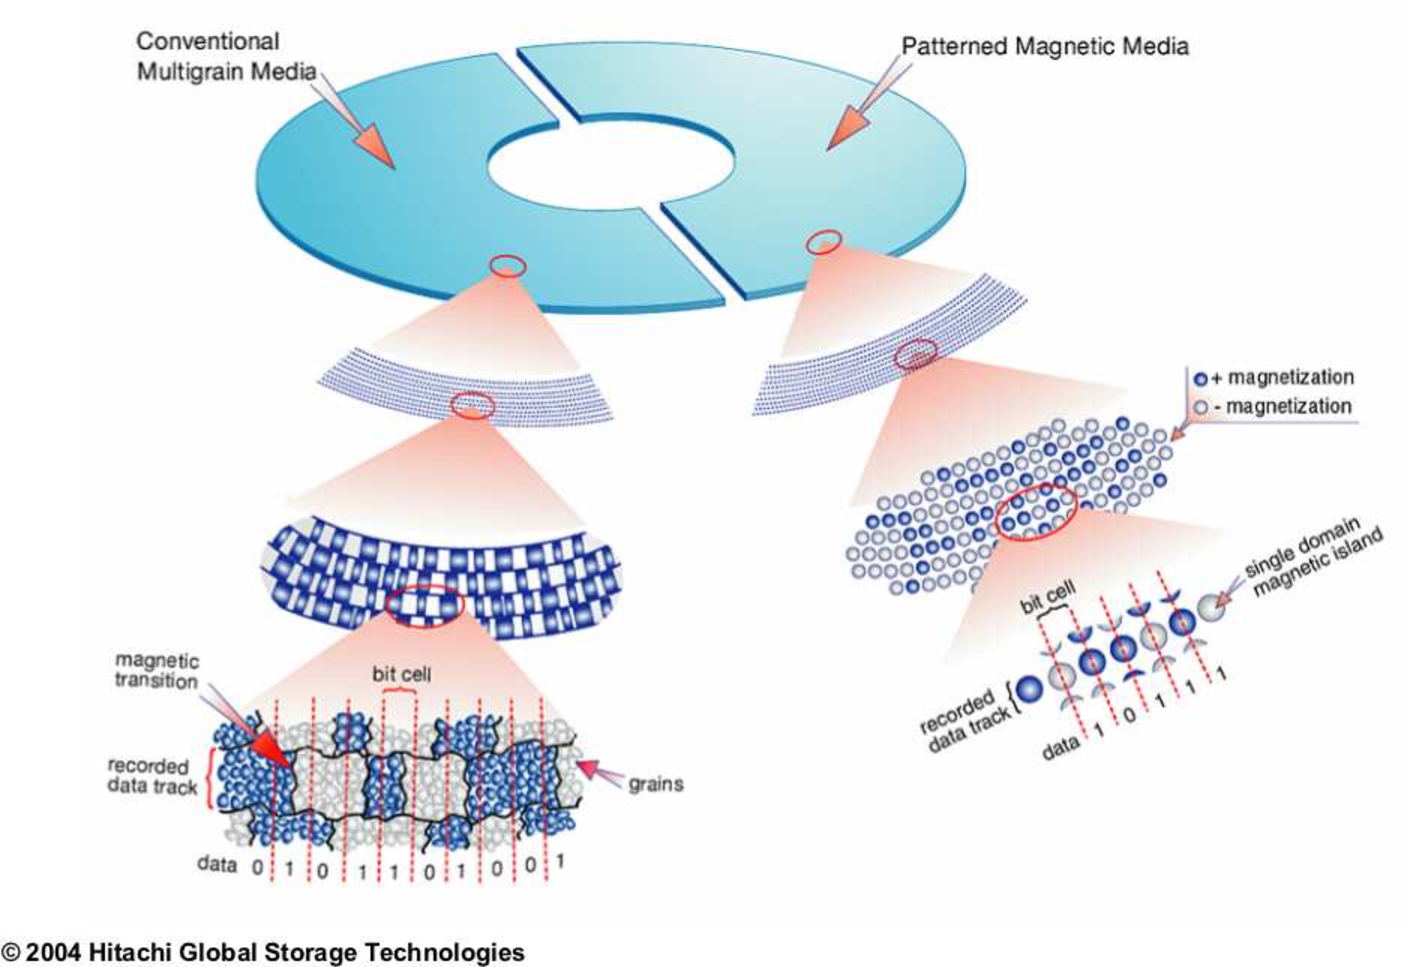
\includegraphics[width=0.75\textwidth]{./images/conventional_vs_pattern_media}
  \caption{Different media types for magnetic data storage. Conventional multigrain media is
    the layout used in current hard disk drives. Bit pattern media is a potential new layout which could allow for further scaling up of data density.
    \cite{conventional_vs_patterned_media} \label{fig:Layouts-for-magnetic}}
\end{figure}

\section{Mathematical Description of the Trilemma}

We present a very simple description of how the areal density of a disk depends on the three factors mentioned in Section~\ref{sec:hard-disk-drives}.

The anisotropy of a material refers to its preference for magnetisation along one axis (typically in either direction), often called the \emph{easy axis}. There are various types of anisotropy, caused by different effects. The most important is magnetocrystalline anisotropy which is caused by the crystal structure of the material affecting the electrons resulting in preferred spin directions.\cite{Getzlaff2008}

In the absence of an applied field the magnetocrystalline anisotropy
causes an energy barrier between opposite magnetisations. A useful
quantity is $K$, the energy per unit volume required to overcome
this energy barrier and flip the magnetisation direction. When writing
to a grain the applied field must overcome the energy barrier before
switching the magnetisation. Thus an applied field

\begin{equation}
\Happ > \dfrac{2K}{\mu_{0}M_s},
\label{eq:43}
\end{equation}

is needed, where $M_s$ is the saturation magnetisation of the material and $\mu_0 = 4 \pi \E{-7} \text{N A}^{-2}$ is the magnetic constant.\cite{McDaniel2005}

A good measure of thermal stability is the ratio between the energy required to
flip the magnetisation of a grain, $KV$ (where $V$ is the grain volume) and the
thermal energy $k_{B}T$ ($k_{B}$ is Boltzmann's constant, $T$ is the temperature
in Kelvin)

\begin{equation}
  \eta_{0}=\dfrac{KV_{grain}}{k_{B}T}.\label{eq:eta}
\end{equation}
For acceptable thermal stability with a typical distribution of grain
volumes $\eta_0 \gtrsim 60$ is required.\cite{McDaniel2005}

For a disk with $N$ grains per bit, grain thickness $\delta$ and packing
fraction $p$ (the ratio of magnetic to non-magnetic areas of the
disc) the area per bit is
\[
A_{bit}=\dfrac{N}{p}\cdot A_{grain}=\dfrac{N}{p}\cdot\dfrac{V_{grain}}{\delta}
\]

The areal density $D$ of a disk is the inverse of the area per bit,
hence
\[
D=A_{bit}^{-1}=\dfrac{p\delta}{NV_{grain}}.
\]

Finally, substituting in $V_{grain}=\dfrac{\eta_{0}k_{B}T}{K}$ from \eqref{eq:eta} gives
\begin{equation}
D=\dfrac{p\delta}{k_{B}T}\cdot\dfrac{K}{N\eta_{0}}.\label{eq:AD}
\end{equation}


From \eqref{eq:AD} we see which factors can be scaled to increase the areal
density of a disk, but some of these factors can be immediately ruled
out. Cooling of hard drives (i.e. reduction of $T$) is probably not an option
for any real world applications because the small improvement in stability (and
hence areal density) that could be gained is vastly outweighed by inconvenience
and cost of cooling. The track depth $\delta$ cannot be increased beyond twice
the bit length because multiple domains will start to form in the vertical
direction \cite{McDaniel2005} and also reducing the track depth can degrade
performance\cite{Litvinov2002}. Reducing the packing fraction can only lead to a
small areal density increase because most of the disk already consists of
magnetic material.

This leaves the anisotropy $K$, the number of grains per bit $N$ and the thermal
stability $\eta_{0}$ as possible scaling factors.  However, the signal to noise
ratio depends on the sharpness of the boundaries between bits, which is
dependant on the number of grains per bit. Fewer grains per bit results in a
rougher bit boundary and hence more noise. Additionally the thermal stability is
proportional to the grain volume. Hence we are left with a trade off between
signal to noise ratio, thermal stability and writability: the trilemma.

Bit pattern media sidesteps the problem by removing the dependence
of signal to noise ratio on $N$ and reducing $N$ to one. The signal
to noise ratio is then dominated by how well the actual island locations
correspond to their theoretical locations, which is determined by
the manufacturing process. It has been demonstrated that the signal
to noise ratio for bit pattern media can be at least as low as in
traditional media.\cite{Moritz2004}

Thermally assisted recording allows for a large increase in stability while maintaining writability because the value of $K$ at high temperatures (i.e. when writing) is typically far lower than at room temperature (i.e. when thermal stability is needed).

The model presented above is a vast simplification of the actual magnetisation process. For example, inter-grain effects, time dependence and grain shape have all been ignored. However it is still useful to see that there is a trade-off between the various factors and to understand how bit pattern media and heat assisted magnetic recording can help circumvent some of the problems.


%%% Local Variables:
%%% mode: latex
%%% TeX-master: "main"
%%% End:


%% \section{Longitudinal and Perpendicular Recording}
\label{sec:long-perp-record}

The magnetic grains used to store data in hard drives can be aligned such that
their easy axes (the direction in which they are most easily magnetised) point
in the direction either along (longitudinal) or perpendicular to the disk
surface. This section aims to discuss the differences between the two cases.

Most of the fundamentals of perpendicular recording were introduced in the 1970s
by Iwasaki et. al.\cite{Piramanayagam2009a} but until recently almost all hard
disk drives used longitudinal recording.  This was partly because of problems
with noise in perpendicular media which were only resolved in
2000\cite{Piramanayagam2009a} and partly because there was no need for such a
fundamental change as improvements in longitudinal recording technology allowed
for consistently increasing areal densities.

As discussed in Section~\ref{sec:hard-disk-drives}, the areal density of hard
drives is approaching a fundamental limit known as the superparamagnetic
limit. Perpendicular recording has helped to delay it in two ways. Firstly, due
to geometry it allows the same write head magnetisation to create a stronger
field in the recording medium. Secondly, it results in the bits being arranged
such that they are more likely to reinforce each others' magnetisation, giving
better stability.

The major differences between longitudinal and perpendicular recording are
illustrated in Figure~\ref{fig:Longitudinal-perpendicular}. In particular, in
perpendicular recording, the shape of the write head is changed and a soft magnetic
underlayer is added.

\begin{figure}[!ht]
  \center
  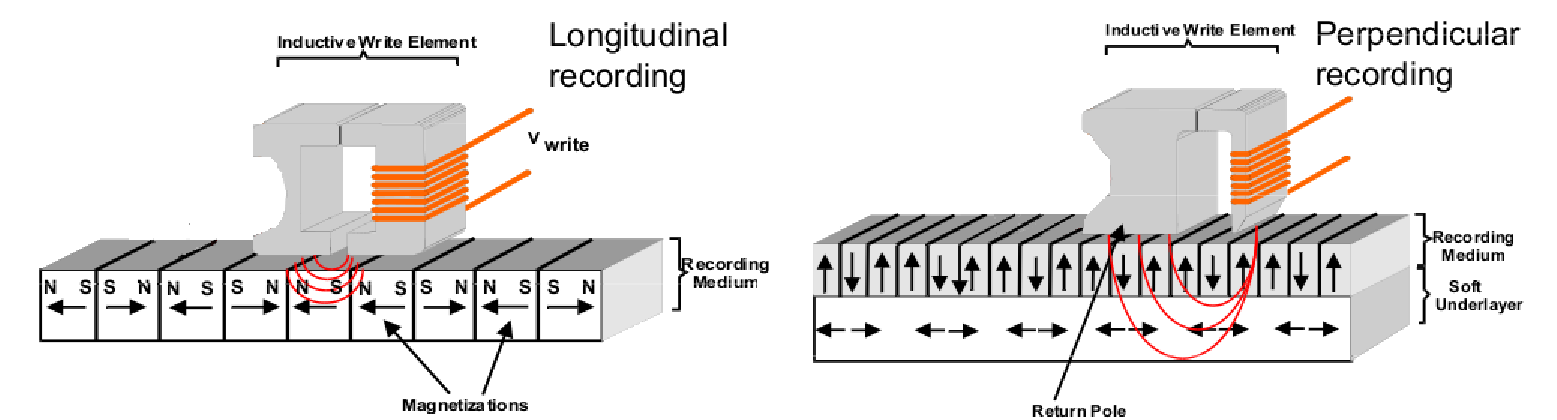
\includegraphics[width=1\textwidth]{./images/perphead}
  \caption{The write head set up for longitudinal and perpendicular recording.
    Image modified from
    \cite{LongitudinalPerpDiagram}.}
  \label{fig:Longitudinal-perpendicular}
\end{figure}

\subsection{Write Heads}

\subsubsection{Write Head Arrangements}

As shown in Figure~\ref{fig:Longitudinal-perpendicular} the write head is
arranged differently in longitudinal and perpendicular recording.

Longitudinal recording requires a \emph{ring head}. At a basic level it consists
of a ring of soft magnetic material with a coil of wire around it and a small
gap in the ring near surface of the disk. When current flows through the wire it
magnetises the ring. This magnetisation can be thought of as magnetic flux
flowing around the ring, at the gap the flux spreads out causing a ``fringing
field'' in the surrounding area. This is the field that is used to write to the
recording media.\cite{Khizroev2004a}

A similar head can be used for perpendicular recording, but because of the
orientation of the magnetisation a better option is available: a \emph{single
  pole head }(SPH). A single pole head consists of a roughly semicircular piece
of soft magnetic material with a coil around it above the disk and a \emph{soft
  magnetic underlayer} (SUL) below the recording layer.  Magnetic flux flows
around the semicircular head and directly through the recording layer before
being redirected back to the other end of the head by the soft underlayer. If
one of the poles of the head is made much narrower than the other then flux is
concentrated below the narrow pole but spread out below the other pole. This
means that only the narrow pole has a strong enough field to write to the disk
-- hence the name.\cite{Khizroev2004a}

A good way to think about the soft underlayer is to use the method of images,
similar to that used for conductors in electrostatics. \cite{Hoinville2002}
According to this method the effect of an ideal (infinitely thick with infinite
permeability) soft underlayer is the same as that of a mirror image of the real
write head (with the line of symmetry at the surface of the soft underlayer)
with ``magnetic charges'' of the opposite sign, as shown in
Figure~\ref{fig:imaginary_head}. In this approximation a single pole head with a
soft magnetic underlayer is similar to a ring head except that the writing takes
place directly within the gap rather than outside it.\cite{Richter2007a}

\begin{figure}[!ht]
  \center
  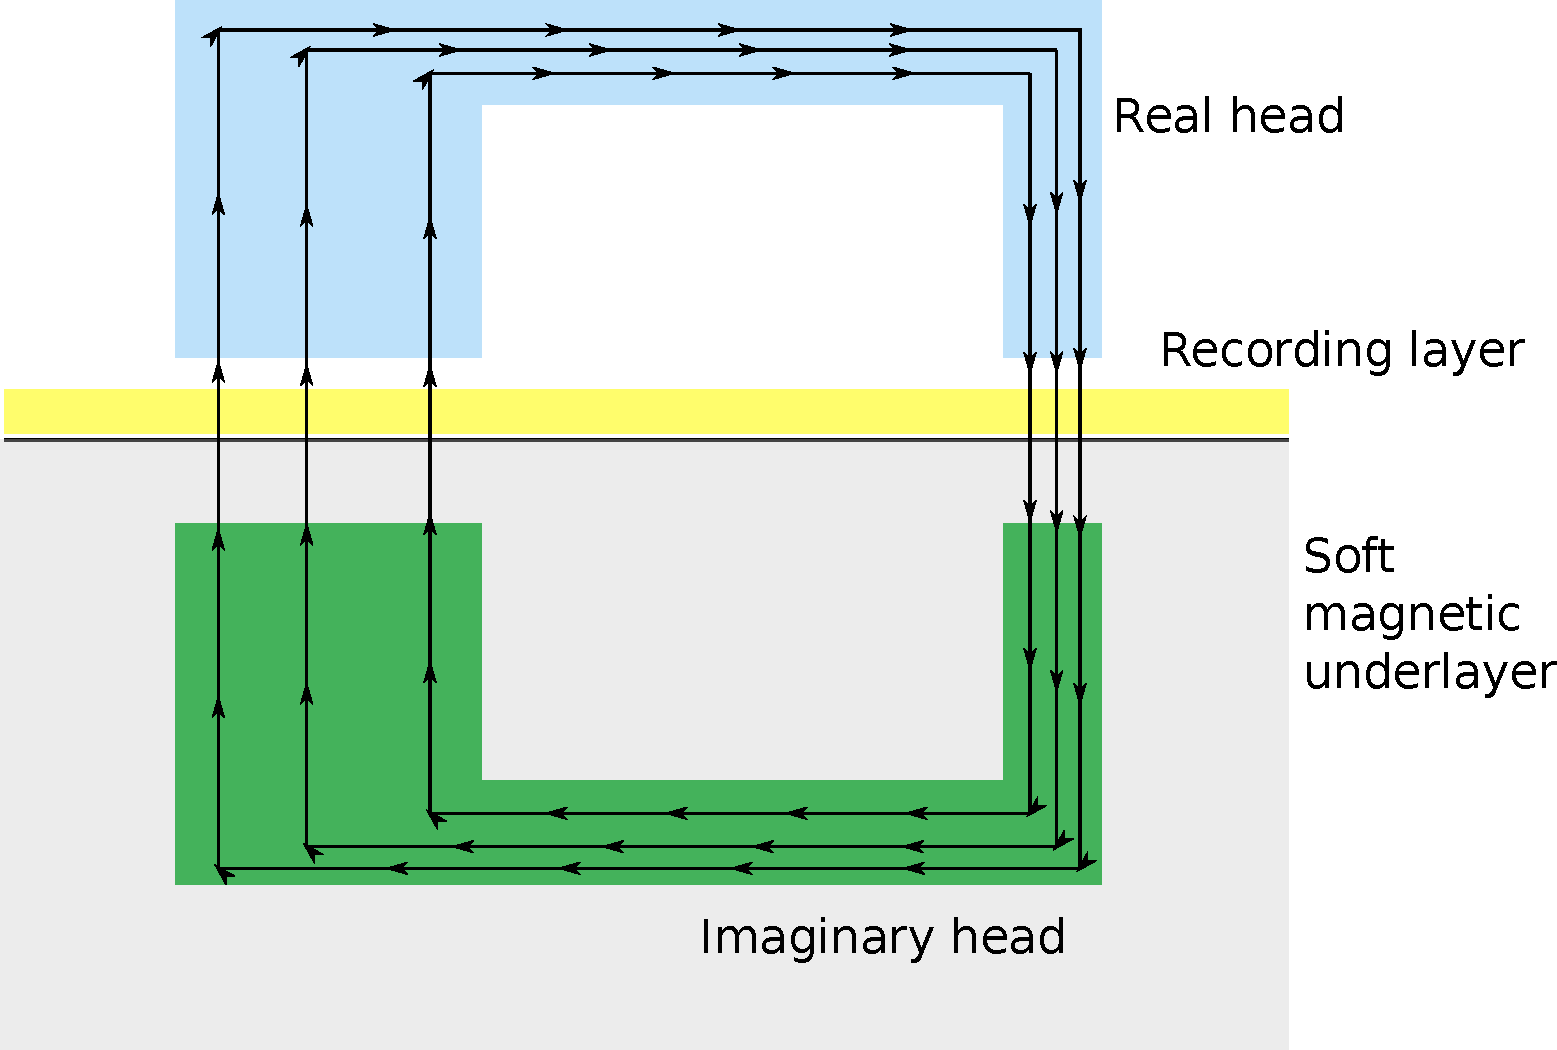
\includegraphics[width=0.75\textwidth]{./images/SPH_images}
  \caption{A single pole head along with its image in a soft magnetic underlayer
    with magnetic flux line shown.\label{fig:imaginary_head}}
\end{figure}


\subsubsection{Effects on the applied write field}

The write field (in the recording direction) at a point on the recording medium
is related to the solid angle filled by the write head (in steradians),
$\omega$, and the magnetisation of the write head in the recording direction,
$M_{z}$ by\cite{Richter2007a}
\[ H_{z}=\dfrac{M_{z} \omega}{4\pi}.\]

As a simple model we assume that the write head extends infinitely both along
and across the track (i.e. in the $x$ and $y$ directions). Then for a ring head
the solid angle is $\omega=2\pi$ sr, corresponding to the entire top hemisphere
being filled. By comparison for a single pole the solid angle is $\omega=4\pi$
sr because the top hemisphere is filled by the real head and the bottom
hemisphere is filled by the imaginary head created by the soft underlayer. Hence
in this approximation the applied field for a single pole head is double the
applied field for a ring head. Obviously real write heads are finite but single
pole heads still produce approximately double the applied field for the same
head magnetisation.\cite{Khizroev2004a} As mentioned previously in
Section~\ref{sec:trilemma} an increase in the write field allows the use of
higher anisotropy materials in the recording layer which increases the thermal
stability of bits allowing an increase in areal density.


\subsection{Magnetostatic Fields}

The magnetostatic field of a magnetised body is the field created by the body
itself. This field affects the magnetisation of the body leading to complex
interactions. The magnetostatic field is also known as the demagnetising field
(because it tends to oppose the magnetisation of the body creating it) or the
stray field. It is the cause of shape anisotropy -- the shape of a magnetic body
affects the magnetostatic field and hence can sometimes give a preferred
magnetisation direction.

A simple way to think about the magnetostatic field is to use poles. When a
piece of ferromagnetic material is magnetised poles are created at the ends
causing a magnetostatic field ($\Hms$) opposing the magnetisation within the
material. As a simple rule of thumb the strength of $\Hms$ is inversely
proportional to the separation of the magnetic poles. \cite{Piramanayagam2007a}

\begin{figure}[!ht]
  \center
  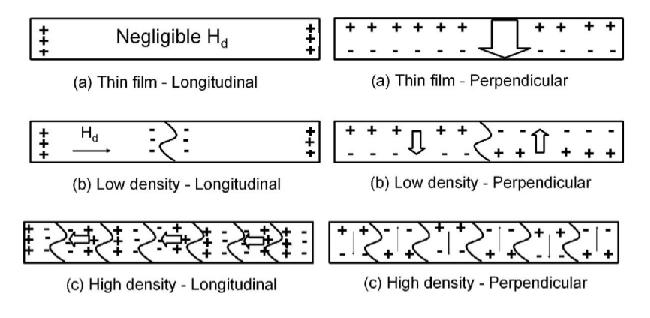
\includegraphics[width=0.8\textwidth]{./images/demagsimple}
  \caption{
    A simple picture of magnetic charges in longitudinal and perpendicular
    recording media. The thickness of the arrows show the strength of the
    internal magnetostatic field.  Modified from Piramanayagam
    2007. \cite{Piramanayagam2007a}}
  \label{fig:simple-picture-demag}
\end{figure}


\subsubsection{Differences in Internal Magnetostatic Field Between Perpendicular and Longitudinal Recording}
\label{sec:diff-intern-magn}
We first focus on the internal magnetostatic field -- the effect of the magnetisation of a body (or a bit in magnetic data storage) on itself.

Strong internal magnetostatic fields can cause problems in magnetic data storage
because they work against the anisotropy of the ferromagnetic grains, reducing
the thermal stability of the grains. This effect cannot be counteracted simply
by increasing the anisotropy because the magnetostatic field is
non-constant. Hence it is preferable to keep the internal magnetostatic fields
as small as possible.

A simple idea of the differences in internal magnetostatic field strength between
longitudinal and perpendicular recording can be seen by examining the
distribution of magnetic poles. A comparison of the two is shown in Figure
\ref{fig:simple-picture-demag}. For low linear data densities (i.e. large bit areas)
and thin films longitudinal recording has a larger separation of the magnetic
poles that cause the internal magnetostatic field, hence longitudinal recording has a
lower internal magnetostatic field. At high linear data densities and/or thicker films
perpendicular recording gives a lower internal magnetostatic field for the same
reason.\cite{Piramanayagam2007a}

\begin{figure}[!ht]
  \center
  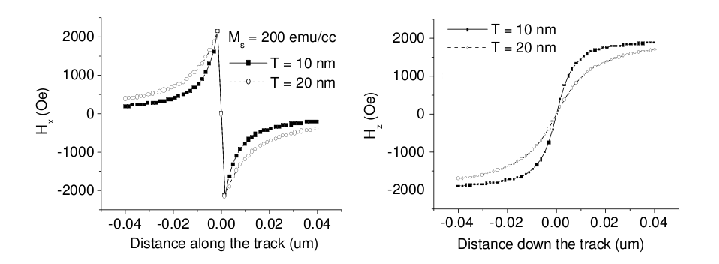
\includegraphics[width=1\textwidth]{./images/perpvslongdemags}
  \caption{Calculated magnetostatic fields near a single ideal transition for
    longitudinal (left) and perpendicular (right) recording. The perpendicular
    recording calculation assumes an ideal soft underlayer. The grey line on each
    graph corresponds to a thicker magnetic recording layer. Modified from Litvinov
    2002\cite{Litvinov2002}.}
  \label{fig:Calculated-demagnetising-fields}
\end{figure}

The magnetostatic fields can be more precisely calculated from the magnetic
charge distributions. Plots of these calculations of the magnetostatic fields at
the centre of the recording layer near an ideal transition (a change in the
magnetisation direction) are shown in Figure
\ref{fig:Calculated-demagnetising-fields}. It can be seen that the field
decreases near the point of the transition for the perpendicular case whereas
for the longitudinal case it reaches a maximum. This implies a lower
magnetostatic field for perpendicular recording at short bit lengths (i.e. high
areal density). Also the magnetostatic field decreases for thicker recording
layers in perpendicular recording while the opposite happens in the longitudinal
case. Hence this more advanced description agrees with the simple explanation
given above.\cite{Litvinov2002}

In the case that neighbouring tracks have opposite magnetisation the
magnetostatic field also decreases with track density. However encoding data to
arrange this scenario causes too large a decrease in storage capacity to be
useful. \cite{Litvinov2002}

\begin{figure}
  \begin{center}
    \hspace{-5em} % Manual centering...
    % GNUPLOT: LaTeX picture with Postscript
\begingroup
  \makeatletter
  \providecommand\color[2][]{%
    \GenericError{(gnuplot) \space\space\space\@spaces}{%
      Package color not loaded in conjunction with
      terminal option `colourtext'%
    }{See the gnuplot documentation for explanation.%
    }{Either use 'blacktext' in gnuplot or load the package
      color.sty in LaTeX.}%
    \renewcommand\color[2][]{}%
  }%
  \providecommand\includegraphics[2][]{%
    \GenericError{(gnuplot) \space\space\space\@spaces}{%
      Package graphicx or graphics not loaded%
    }{See the gnuplot documentation for explanation.%
    }{The gnuplot epslatex terminal needs graphicx.sty or graphics.sty.}%
    \renewcommand\includegraphics[2][]{}%
  }%
  \providecommand\rotatebox[2]{#2}%
  \@ifundefined{ifGPcolor}{%
    \newif\ifGPcolor
    \GPcolorfalse
  }{}%
  \@ifundefined{ifGPblacktext}{%
    \newif\ifGPblacktext
    \GPblacktexttrue
  }{}%
  % define a \g@addto@macro without @ in the name:
  \let\gplgaddtomacro\g@addto@macro
  % define empty templates for all commands taking text:
  \gdef\gplbacktext{}%
  \gdef\gplfronttext{}%
  \makeatother
  \ifGPblacktext
    % no textcolor at all
    \def\colorrgb#1{}%
    \def\colorgray#1{}%
  \else
    % gray or color?
    \ifGPcolor
      \def\colorrgb#1{\color[rgb]{#1}}%
      \def\colorgray#1{\color[gray]{#1}}%
      \expandafter\def\csname LTw\endcsname{\color{white}}%
      \expandafter\def\csname LTb\endcsname{\color{black}}%
      \expandafter\def\csname LTa\endcsname{\color{black}}%
      \expandafter\def\csname LT0\endcsname{\color[rgb]{1,0,0}}%
      \expandafter\def\csname LT1\endcsname{\color[rgb]{0,1,0}}%
      \expandafter\def\csname LT2\endcsname{\color[rgb]{0,0,1}}%
      \expandafter\def\csname LT3\endcsname{\color[rgb]{1,0,1}}%
      \expandafter\def\csname LT4\endcsname{\color[rgb]{0,1,1}}%
      \expandafter\def\csname LT5\endcsname{\color[rgb]{1,1,0}}%
      \expandafter\def\csname LT6\endcsname{\color[rgb]{0,0,0}}%
      \expandafter\def\csname LT7\endcsname{\color[rgb]{1,0.3,0}}%
      \expandafter\def\csname LT8\endcsname{\color[rgb]{0.5,0.5,0.5}}%
    \else
      % gray
      \def\colorrgb#1{\color{black}}%
      \def\colorgray#1{\color[gray]{#1}}%
      \expandafter\def\csname LTw\endcsname{\color{white}}%
      \expandafter\def\csname LTb\endcsname{\color{black}}%
      \expandafter\def\csname LTa\endcsname{\color{black}}%
      \expandafter\def\csname LT0\endcsname{\color{black}}%
      \expandafter\def\csname LT1\endcsname{\color{black}}%
      \expandafter\def\csname LT2\endcsname{\color{black}}%
      \expandafter\def\csname LT3\endcsname{\color{black}}%
      \expandafter\def\csname LT4\endcsname{\color{black}}%
      \expandafter\def\csname LT5\endcsname{\color{black}}%
      \expandafter\def\csname LT6\endcsname{\color{black}}%
      \expandafter\def\csname LT7\endcsname{\color{black}}%
      \expandafter\def\csname LT8\endcsname{\color{black}}%
    \fi
  \fi
  \setlength{\unitlength}{0.0500bp}%
  \begin{picture}(9070.00,4534.00)%
    \gplgaddtomacro\gplbacktext{%
      \csname LTb\endcsname%
      \put(946,704){\makebox(0,0)[r]{\strut{} 0}}%
      \put(946,1417){\makebox(0,0)[r]{\strut{} 0.2}}%
      \put(946,2130){\makebox(0,0)[r]{\strut{} 0.4}}%
      \put(946,2843){\makebox(0,0)[r]{\strut{} 0.6}}%
      \put(946,3556){\makebox(0,0)[r]{\strut{} 0.8}}%
      \put(946,4269){\makebox(0,0)[r]{\strut{} 1}}%
      \put(1078,484){\makebox(0,0){\strut{} 0}}%
      \put(1690,484){\makebox(0,0){\strut{} 0.2}}%
      \put(2302,484){\makebox(0,0){\strut{} 0.4}}%
      \put(2914,484){\makebox(0,0){\strut{} 0.6}}%
      \put(3526,484){\makebox(0,0){\strut{} 0.8}}%
      \put(4138,484){\makebox(0,0){\strut{} 1}}%
      \put(176,2486){\rotatebox{-270}{\makebox(0,0){\strut{}$\dfrac{-H_{m,x}}{M_s}$}}}%
      \put(2608,154){\makebox(0,0){\strut{}$\rho$}}%
    }%
    \gplgaddtomacro\gplfronttext{%
    }%
    \gplgaddtomacro\gplbacktext{%
      \csname LTb\endcsname%
      \put(5481,704){\makebox(0,0)[r]{\strut{} 0}}%
      \put(5481,1417){\makebox(0,0)[r]{\strut{} 0.2}}%
      \put(5481,2130){\makebox(0,0)[r]{\strut{} 0.4}}%
      \put(5481,2843){\makebox(0,0)[r]{\strut{} 0.6}}%
      \put(5481,3556){\makebox(0,0)[r]{\strut{} 0.8}}%
      \put(5481,4269){\makebox(0,0)[r]{\strut{} 1}}%
      \put(5613,484){\makebox(0,0){\strut{} 0}}%
      \put(6225,484){\makebox(0,0){\strut{} 0.2}}%
      \put(6837,484){\makebox(0,0){\strut{} 0.4}}%
      \put(7449,484){\makebox(0,0){\strut{} 0.6}}%
      \put(8061,484){\makebox(0,0){\strut{} 0.8}}%
      \put(8673,484){\makebox(0,0){\strut{} 1}}%
      \put(4711,2486){\rotatebox{-270}{\makebox(0,0){\strut{}$\dfrac{-H_{m,z}}{M_s}$}}}%
      \put(7143,154){\makebox(0,0){\strut{}$\rho$}}%
    }%
    \gplgaddtomacro\gplfronttext{%
    }%
    \gplbacktext
    \put(0,0){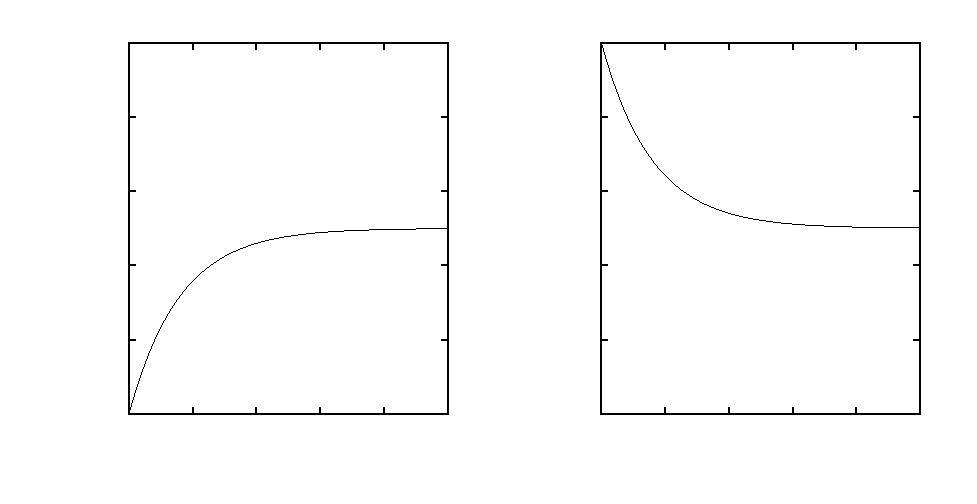
\includegraphics{external_field_at_surface}}%
    \gplfronttext
  \end{picture}%
\endgroup
 
    %??ds broken, probably need to redo if this gets included anywhere...
    \caption{Normalised magnetostatic fields for longitudinal (left) and perpendicular (right) recording at the surface of the recording layer as a function of $\rho$ (the ratio of bit thickness to bit length).}
    \label{fig:surface-demag}
  \end{center}
\end{figure}

\subsubsection{External Magnetostatic Fields}
\label{sec:Stray-fields}

The external magnetostatic field is important in magnetic data storage because
it is the field detected by the read head when data is being read from the
disc. \cite{Richter1999}

A good measure of the strength of the field at the read head is the strength of
the internal magnetostatic field at the surface of the disk. For the case of a
sinusoidally varying magnetisation (i.e. the binary pattern 01010101) the bit
density can be written as $\rho=\dfrac{\delta}{\lambda}$ where $\lambda$ is the
wavelength of the sinusoidal variation and $\delta$ is the thickness of the recording
layer. The magnetostatic field at the surface of the disk is then
\[ H_{m,x}=-\frac{M_s}{2}(1-e^{-2\pi\rho}),\]
in the $x$ direction for the longitudinal case and
\[ H_{m,z}=-\frac{M_s}{2}(1+e^{-2\pi\rho}),\]
in the $z$ direction for the perpendicular case. \cite{Richter1999}


Figure~\ref{fig:surface-demag} shows plots of $H_{m,x}$ and $H_{m,z}$ against
$\rho$. Note that for reasonably large $\rho$ (i.e. for bits that are shorter in
length than the thickness of the recording layer) both fields approach
$H_{m}=-\dfrac{M}{2}$. For almost any realistic case the strength of the
magnetostatic field near the read head is no different between the two recording
orientations. Hence in this approximation there is no difference in signal
strength between the two types of recording media. A more detailed comparison by
Litvinov \cite{Litvinov2005a} showed that using perpendicular recording actually
gives a higher signal strength, mostly due to the soft underlayer.

\begin{figure}
  \center
  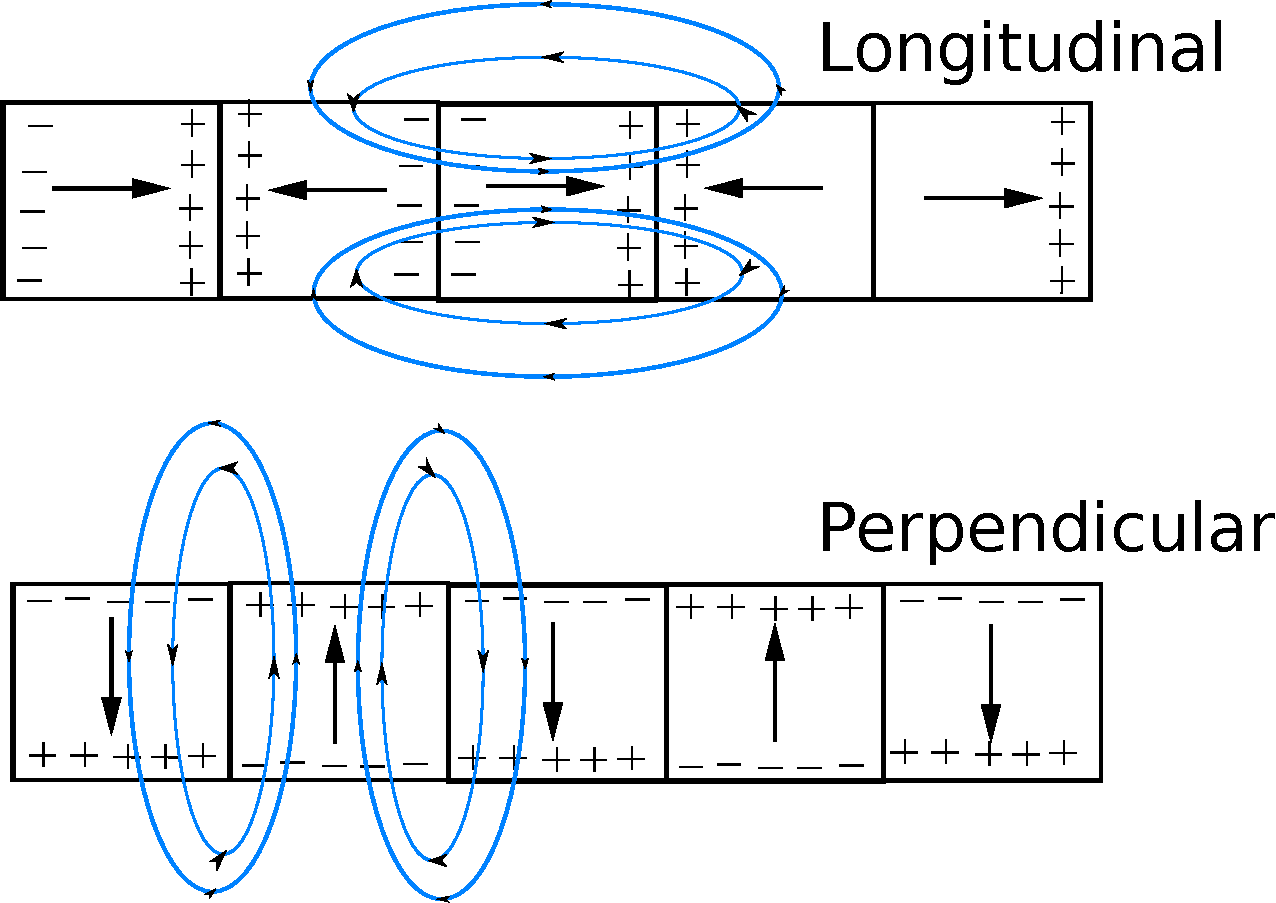
\includegraphics[width=0.8\textwidth]{./images/strayfielddiffs}
  \caption{Stray field directions in longitudinal and perpendicular
    recording.}
  \label{fig:Stray-field-directions}
\end{figure}

% you should add a citation for  "However by encoding the data we can obtain a recording that largely consists of alternating bits without too much loss of areal density, and this encoding is regularly used for other reasons'' if still in the thesis
The external magnetostatic field effects on neighbouring bits in longitudinal
and perpendicular recording are shown in Figure
\ref{fig:Stray-field-directions}. From this we can see that as long as
transitions are fairly common the magnetostatic field from nearby bits actually
reinforce each other in the perpendicular media case. Conversely, for the same
pattern, the fields created by bits in longitudinal media act against the
magnetisation of neighbouring bits. Naively this would appear to be of no use
since real data do not always form an alternating pattern. However data is
typically encoded such that it largely consists of alternating bits for other
reasons. Hence the magnetostatic fields in perpendicular recording actually
increase thermal stability of neighbouring bits but decrease stability in
longitudinal recording.


%%% Local Variables:
%%% mode: latex
%%% TeX-master: "main"
%%% End:


\chapter{Continuous Micromagnetics}
\label{sec:cont-micromag}

In this section we give an introduction to micromagnetics including a statement of the equations to be solved.

\section{Definitions}
We use S.I. units throughout unless otherwise specified. In particular normalised quantities are no longer in S.I. units.

We define $\Hv(\xv,t)$ to be the magnetic field at position $\xv$ and time $t$ in units of $\Hu$.

We define $\Mv(\xv,t)$ to be a vector field representing the expectation value of the magnetisation per unit volume averaged over a number of unit cells.\cite{Aharoni1996}
The units of $\Mv$ are $\Mu$, the length of $\Mv(\xv,t)$ is given by the saturation magnetisation $M_s$.
At zero temperature $M_s$ is a fixed parameter of the material but in finite temperature models $M_s$ may vary.

These quantities are related to the magnetic flux density $\Bv(\xv,t)$ (in units of $\Bu$) by
\begin{equation}
  \label{eq:37}
  \Bv(\xv,t) = \mu_0 \left( \Hv(\xv,t) + \Mv(\xv,t) \right),
\end{equation}
% \cite{Gilbert2004} says that this magnetisation is different - averaged over all material rather than over a few cells...
where $\mu_0$ is the magnetic constant (or permeability of free space).

In general we will not make dependencies on $\xv$ and $t$ explicit.

\section{Energy of a Magnetic Body}
\label{sec:energy-magnetic-body}

The effects that must be considered in a micromagnetic mode are: the magnetostatic self field, the exchange energy and the magnetocrystalline anisotropy energy. Also important is the external applied field due to magnetic bodies or electrical currents outside the modelled region. Other effects which are sometimes important include temperature (thermal effects) and magnetostriction energy (due to stretching or compressing the magnet).

We begin by providing a description of each of these effects and their contribution to the total energy density, $E$. We can get the effective fields given by these energies by taking
\begin{equation}
  \Hv = \dfrac{-1}{\mu_0 V_{\magd}} \dfrac{\delta E}{\delta \Mv},
\end{equation}
where $\delta$ indicates a variational derivative and $V_{\magd}$ is the volume of the magnetic domain. ??ds citation? Is this correct?

%% Energy and field expressions below are taken from Matteo Franchin's thesis.\cite{Franchin2009}\footnote{Note that due to the variety in unit systems, definitions of magnetisation and other choices it can be difficult to compare energy/effective field equations from different authors, in particular the location of factors of $\mu_0$.}

\subsection{Exchange Energy}

In a ferromagnetic material neighbouring magnetic moments prefer to align parallel to each other due to quantum mechanical effects. This can be well approximated by a classical expression for exchange energy:\cite{Aharoni1996}
\begin{equation}
  \label{eq:39}
  \Eex =  \frac{\Exchc}{M_s^2} \int_{\magd} (\nabla M_x)^2  + (\nabla M_y)^2  + (\nabla M_z)^2 \d \magd,
\end{equation}
where $A$ is the material dependant exchange constant which depends on the crystal structure and the strength of the exchange coupling between electrons in the material.

We write the vector Laplacian as $\lap \Mv = (\lap M_x,\lap M_y, \lap M_z )$. Then the exchange effective field is given by
\begin{equation}
  \label{eq:Hex}
  \Hex = \frac{2 \Exchc}{ \mu_0 M_s} \lap \Mv.
\end{equation}

\subsection{Magnetostatic Field}
\label{sec:magnetostatic-field}

Magnetic materials generate magnetic fields, which in turn affects the magnetic material. This type of field is also known as the demagnetising field since it tends to oppose the magnetisation of the body. The magnetostatic field, $\Hms$, can be calculated in two ways: an integral based method or a potential based method. These methods are discussed in \autoref{sec:magstat-field-calc-inte} and \ref{sec:magstat-field-calc-pote} respectively.

Once the self field has been calculated the energy contribution due to it is given by
\begin{equation}
  \label{eq:41}
  \Ems =  \frac{-\mu_0}{2} \int_{\magd} \Mv \cdot \Hms \d \magd,
\end{equation}
where the factor of $\frac{1}{2}$ is to avoid double counting.

The integral form of the magnetostatic field at a point $\xv \in \real^d$ due to the magnetic body $\magd$ with boundary $\boundd$ can be given in terms of magnetisation $\Mv$ by an integral over all volume and surface ``magnetic charges'' ($\nabla \cdot \Mv(\xv)$ and $\Mv(\xv) \cdot \nv(\xv)$ respectively) as
\begin{align}
  \Hms(\xv) &= \frac{1}{4 \pi} \Big[ - \int_\magd \frac{\big( \nabla' \cdot \Mv(\xv') \big)(\xv - \xv')}{\abs{ \xv -\xv'}^3} \d^3 \xv'
              + \int_\boundd \frac{ \big( \Mv(\xv') \cdot \nv(\xv') \big) (\xv - \xv')}{\abs{\xv - \xv'}^3} \d^2 \xv' \Big],
              \label{eq:Hmsint}
\end{align}
where $\nabla'$ denotes the grad operator with respect to the $\xv'$ coordinate.
For completeness we note that single magnetic charges (magnetic monopoles) have not been observed in nature.
However they are a very useful mathematical tool for calculations of magnetic fields.

% Alternatively it can be given in terms of a sum over the dipole fields of magnetic moments (\ie discretised magnetisation) as
% \begin{equation}
%   \label{eq:9}
%   \Hms(\xv) = \frac{1}{4\pi} \sum_i \frac{1}{|\xv - \xv_i|^3} \Big[ \mu_i(\xv_i) - 3(\mu_i(\xv_i) \cdot \ruv_i ) \cdot \ruv_i \Big],
% \end{equation}
% where $\ruv_i$ is the unit vector pointing from $\xv_i$ to $\xv$.


When the magnetic field is being produced only by magnets and not currents (\ie the magnetic field is irrotational) it is possible to express the field as a function of a scalar potential, $\phim$.\cite{Coey2010}
Let $\magd$ be the magnetic body, $\boundd$ it's boundary and $\nv$ the outward unit normal on the boundary.
Then we have
\begin{gather}
  \Hms = - \nabla \phim,  \label{eq:Hms} \\
  \lap \phim = \nabla \cdot \Mv \quad \xv \in \fulld, \label{eq:nnphim}
\end{gather}
With the following boundary conditions
\begin{gather}
  \phim^\inte - \phim^\exte = 0 \quad \xv \in \boundd, \label{eq:cont-phi-bound} \\
  \pd{\phim^\inte}{\nv} - \pd{\phim^\exte}{\nv} = \Mv \cdot \nv \quad \xv \in \boundd,
  \label{eq:nndphidn-bound} \\
  \phim \rightarrow 0 \text{ as } \abs{\xv} \rightarrow \infty, \label{eq:phi-inf}
\end{gather}
where $\phim^\inte$/$\phim^\exte$ are the values of $\phim$ just inside/outside the domain, $\magd$.


Similarly any external applied field gives an energy contribution of
\begin{equation}
  \label{eq:42}
  \Eapp = - \mu_0 \int_{\magd} \Mv \cdot \Happ \d \magd.
\end{equation}

\subsection{Magnetocrystalline Anisotropy}
\label{sec:magn-anis}

Many magnetic materials have a preferred direction (or directions) of magnetisation due to their crystal structure. This is known as magnetocrystalline anisotropy. The equation for the magnetocrystalline anisotropy energy depends on the crystal structure of the material.

A detailed description of the many varieties of magnetocrystalline anisotropy is beyond the scope of this report but can be found in various textbooks on magnetic materials.\cite{Coey2010}\cite{Aharoni1996} However, since the anisotropy term is always a simple function of $\Mv$ it is not important for the implementation of a numerical model which type is used. Hence we give only the most useful case: in magnetic data recording we are interested in materials with a single \emph{easy axis} either in the plane of the disk or perpendicular to it since magnetisation is most stable in these types of material. The first order approximation for the free energy contribution for a perpendicular uniaxial material is given by
\begin{equation}
  \Eca = -K_u \int_\magd \left( \mv \cdot \ev \right)^2 \d \magd,
  \label{eq:36}
\end{equation}
where $\ev$ is the easy axis and $K_u$ is the (material dependant) first order anisotropy energy density coefficient.\footnote{It is possible to define many different forms for this energy. Be warned that the choice of definition changes the meaning of $K_u$!} The first order approximation is valid when the anisotropy energy density coefficients are such that $K_u = K_1 >> K_2$, which is the case in most materials.\cite{Kronmuller2003} The effective field corresponding to this case is
\begin{equation}
  \Hca = \frac{2 K_u}{\mu_0 M_s} \left( \mv \cdot \ev \right) \; \ev.
  \label{eq:Hca}
\end{equation}


\section{Core Models}
??ds before energy/fields?

The general aim of a micromagnetic model is to predict the behaviour of a magnetic body under a variety of conditions. This can either be done by finding the minimum energy of the body or by modelling the dynamics of the magnetisation.

\begin{figure}[ht!]
  \centering
  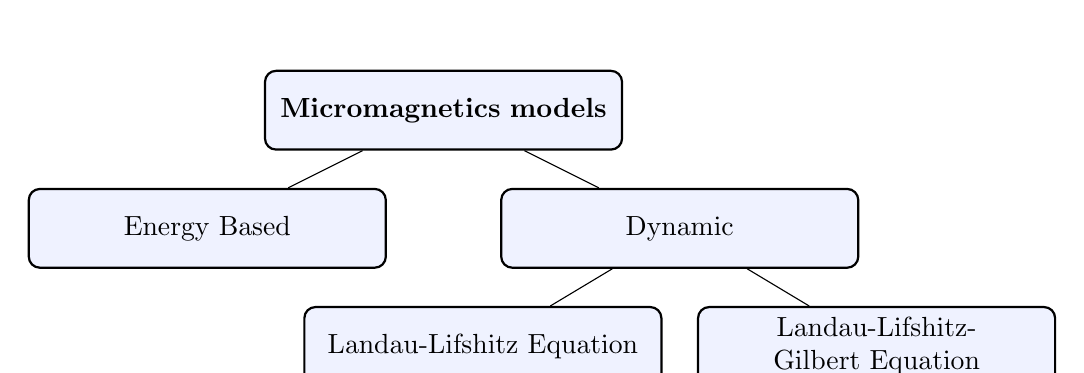
\begin{tikzpicture}[level 1/.style={sibling distance=6cm},
    level 2/.style={sibling distance=5cm}]
    \node[block] {\textbf{Micromagnetics models}}
    child {node[block] {Energy Based}}
    child {node[block] {Dynamic}
      child {node[block] {Landau-Lifshitz Equation}}
      child {node[block] {Landau-Lifshitz-Gilbert Equation}}
    };
  \end{tikzpicture}
  \caption{Possible approaches of a standard numerical micromagnetic model.}
  \label{fig:types-micromag-model}
\end{figure}


\subsection{Energy Based Micromagnetics}
\label{sec:energy-based-micr}

Energy based methods find an equilibrium state of the magnetic system by finding the minimum energy with respect to variation of $\Mv$. For example Fredkin and Koehler used a finite element energy minimisation method.\cite{Koehler1992} Energy based methods require less computational effort than dynamic methods. However they cannot give any information about the time evolution of a system.\cite{Fidler2000} This is an important problem in many areas: for example in magnetic data storage the time taken to reverse the magnetisation of a bit is of key interest.

% could include more details on how to search for minima.

\subsection{Dynamic Micromagnetics}
\label{sec:land-lifsch-gilb}

Dynamic micromagnetic methods model the time evolution of the magnetisation, for given effective field, as a differential equation. Starting with the quantum mechanical angular momentum of an electron, and converting from a single spin a continuous magnetisation gives\cite{Kronmuller2003}
\begin{equation}
  \label{eq:38}
  \dMdt = - \gymagc \Mv \times \Hv,
\end{equation}
where $\Hv$ is the total effective field
\begin{equation}
  \Hv = \Happ + \Hca + \Hex + \Hms.
  \label{eq:Heff}
\end{equation}
Equation~\eqref{eq:38} represents the procession of the magnetisation about the effective field, as shown in \autoref{fig:LLG-terms}. Other effective fields can be added to equation~\eqref{eq:Heff} to model other physical effects such as finite temperature or magnetostriction.

However equation~\eqref{eq:38} implies that the precession motion is undamped, \ie no energy is lost and the magnetisation continues to precess forever. This is obviously not the case so an empirical damping term is added:
\begin{equation}
  \label{eq:LL}
  \dMdt = - \gymagc \Mv \times \Hv - \frac{\dampc \gymagc}{M_s} \Big( \Mv \times (\Mv \times \Hv) \Big),
\end{equation}
where $\dampc$ is an experimentally determined material parameter related to the strength of the damping. Equation~\eqref{eq:LL} is referred to as the Landau-Lifshitz.\cite{Landau1935} The effects of the precession and damping terms are shown in \autoref{fig:LLG-terms}.

\begin{figure}[ht!]
  \centering
  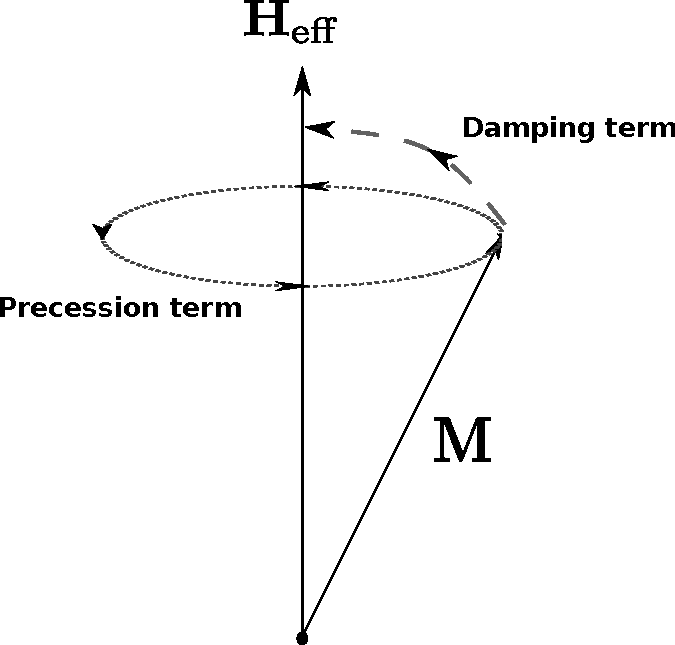
\includegraphics[width=0.6\textwidth]{./images/LLG-terms}
  \caption{The effects of the precession and damping terms in the Landau-Lifshitz and Landau-Lifshitz-Gilbert equations on the magnetisation direction, $\Mv$, of a single magnetic moment with a constant effective field
.}
  \label{fig:LLG-terms}
\end{figure}

However, there are still problems with this equation: for large damping the overall speed of the
motion increases without any increase in the precession speed. Hence the damping dominates and the switching time increases as damping is increased which is physically incorrect.\cite{Mallinson1987} There is another form of equation~\eqref{eq:LL} due to Gilbert\cite{Gilbert2004}, called the Landau-Lifshitz-Gilbert equation, which does not suffer from this problem
\begin{equation}
  \label{eq:Gilbert}
  \dMdt = - \gymagc \Mv \times \Hv + \frac{\dampc}{M_s} (\Mv \times \dMdt),
\end{equation}
where $\dampc \neq \dampc_L$. Equation~\eqref{eq:Gilbert} can be rearranged into the same form as equation~\eqref{eq:LL}, giving
\begin{equation}
  \label{eq:LLG}
  %\tag{LLG}
  \dMdt = \frac{-\gymagc}{1 + \dampc^2} \Big[ (\MxH) + \frac{\dampc}{M_s} \Big(\Mv \times (\MxH) \Big) \Big].
\end{equation}

Equations~\eqref{eq:LL}, \eqref{eq:Gilbert} and \eqref{eq:LLG} link the unknown magnetisation vector as a function of time $\Mv(t)$ with the effective field $\Hv$. To determine $\Mv$ at an arbitrary time $t \neq 0$ we need to integrate one of the above equations with respect to time. This is usually done numerically by employing a time discretisation method as discussed in \autoref{sec:time-discretisation}.

Note that there is no spatial dependence directly contained in equations~\eqref{eq:LL}, \eqref{eq:Gilbert} and \eqref{eq:LLG}. However the exchange effective field and magnetostatic field do contain spatial dependence, so usually the final equation to be solved after all substitutions really is a partial differential equation.

Examples of currently available micromagnetic models include the \texttt{OOMMF}\cite{oommf-website} and \texttt{nmag}\cite{Fischbacher2007} packages, which both use the dynamic method exclusively, along with \texttt{magpar}\cite{Scholz2003} and \texttt{FEMME}\cite{suessco-website} which can use either dynamic or energy based methods.


\subsubsection{Magnetisation boundary conditions}
\label{sec:magn-bound-cond}

The boundary condition on the magnetisation $\mv$ (in dimensional form) is \cite[pgs. 178, 181]{Aharoni1996}
\begin{equation}
  \Mv \times \bigb{ C \dMdn + \pd{w_s}{\Mv}} = \zerov,
\end{equation}
where $C$ is some exchange coeff ??ds and $w_s$ is the surface anisotropy.
Equivalently
\begin{equation}
    \Mv \times \dMdn = \frac{-1}{A} \Mv \times \pd{w_s}{\Mv}.
\end{equation}

For simplicity we commonly consider the case of zero surface anisotropy ($w_s \equiv 0$), in this case the boundary condition becomes
\begin{equation}
  \label{eq:llg-bc}
  \Mv \times \dMdn = \zerov.
\end{equation}
This condition can be arranged into a simpler form: we first note that for equation~\eqref{eq:llg-bc} to hold either $\Mv = \zerov$, $\dMdn = \zerov$ or $\Mv$ is parallel to $\dMdn$.
Clearly $\Mv$ is not the zero vector inside the ferromagnet.
Also we know that the magnetisation length does not change, so $\pd{\Mv}{\av} \cdot \Mv = 0$ for any direction $\av$ (since the change in magnetisation projected onto the magnetisation direction is the change in magnetisation length) hence $\Mv$ and $\dMdn$ cannot be parallel.
So the final boundary condition is simply
\begin{equation}
  \dMdn = \zerov.
\end{equation}


\section{Non-dimensionalisation}
\label{sec:normalisations-appendix}

% ??ds talk about why?

% no unecessary (for the maths) parameters
% improves accuracy by minimising round off error

\subsection{The Landau-Lifshitz-Gilbert equation}
\label{sec:land-lifsh-gilb-normalisation}

We start from the Landau-Lifshitz-Gilbert equation with the magnetostatic, applied, exchange and magnetocrystalline (effective) fields. 
\begin{align}
  \pd{\Mv^*}{t^*} &= - \gymagc \Mv^* \times \Hv^* + \frac{\alpha}{M_s} \Mv^* \times \pd{\Mv^*}{t^*}, \label{eqn:llgnd} \\
  \Hv^* &= \Happ^* - \nabla^* \phi^* + \frac{2\Exchc^*}{\mu_0 M_s} \nabla^{*2} \mv + \frac{2\Kone^*}{\mu_0 M_s} (\mv \cdot \ev) \ev,
          \label{eqn:effnd} \\
  \nabla^{*2} \phi^* &= \nabla^* \cdot \Mv^*, \label{eqn:phind}
\end{align}
where we use $^*$ to denote the dimensional variables, operators and constants that will be non-dimensionalised. We assume for simplicity that $M_s$, $\Exchc$ and $\Kone$ are all
constant throughout the magnetic materials used.

Let
\begin{equation}
  \label{eqn:nddefs}
  \begin{aligned}
    \Mv^* &= M_s \mv,  \\
    \phi^* &= \Phi \phi,  \\
    \Hv^* &= M_s \hv,  \\
    \Kone^* &= \nK \kone,  \\
    t^* &= \frac{1}{\gymagc M_s} t,  \\
    x_i^* &= l x_i. 
  \end{aligned}
\end{equation}
Note that $\Mv$ and $\Hv$ have the same units so we use the same normalisation factor. For dimensional purposes derivatives are equivalent to division by the variable differentiated with respect to, so $\nabla^* = \frac{1}{l} \nabla$, $\pd{a}{t^*} = \gymagc M_s \pd{a}{t}$ etc.

Combining equation~\eqref{eqn:llgnd} with the definitions~\eqref{eqn:nddefs} gives
\begin{equation}
  \notag
  \dmdt \gymagc M_s^2 =
  - \gymagc M_s^2 \mv \times \hv + \frac{\alpha}{M_s} \gymagc M_s^3 \mv \times \dmdt,
\end{equation}

cancelling the various constants results in the non-dimensionalised Landau-Lifshitz-Gilbert equation
\begin{equation}
  \label{eq:53}
  \dmdt = - (\mv \times \hv) + \alpha (\mv \times \dmdt).
\end{equation}

Similarly for equation~\eqref{eqn:phind}
\begin{align*}
  \frac{1}{l^2} \Phi \nabla^{2} \phi &= \frac{1}{l} M_s \nabla \cdot \mv, \\
  \frac{\Phi}{M_s l} \nabla^{2} \phi &= \nabla \cdot \mv.
\end{align*}

Letting $\Phi = M_s l$ we obtain
\begin{equation}
  \label{eq:57}
  \lap \phi = \nabla \cdot \mv.
\end{equation}

Repeating the substitutions for equation~\eqref{eqn:effnd} gives
\begin{align*}
  M_s \hv &= M_s \happ - \frac{\Phi}{l} \nabla \phi + \frac{2 \Exchc }{\mu_0 M_s} \frac{1}{l^2} \lap \mv + \frac{2\kone}{\mu_0 M_s}  \nK (\mv \cdot \ev) \ev, \\
  \hv &= \frac{M_s}{M_s} \happ - \frac{M_s}{M_s} \nabla \phi + \frac{2 \Exchc}{\mu_0 M_s^2} \frac{1}{l^2} \lap \mv + \frac{2\kone}{\mu_0 M_s^2} \nK (\mv \cdot \ev) \ev, \\
  \hv &= \happ - \nabla \phi + \frac{2 \Exchc}{\mu_0 M_s^2} \frac{1}{l^2} \lap \mv + \frac{2\kone}{\mu_0 M_s^2} \nK (\mv \cdot \ev) \ev, \\
\end{align*}

This can be further simplified by choosing the exchange length\footnote{There are actually two exchange lengths: one based on the strength of exchange as compared with the magnetostatic field and another by comparison with the magnetocrystalline anisotropy. We use the magnetostatic-field-based exchange length for normalisation to avoid division by zero in the case of zero magnetocrystalline anisotropy.} as the characteristic length scale
\begin{equation}
  \label{eqn:l-normalisation}
  l = \sqrt{ \frac{2 \Exchc}{\mu_0 M_s^2} },
\end{equation}

and
\begin{equation}
  \label{k-normalisation}
  \nK = \frac{ \mu_0 M_S^2}{2}.
\end{equation}

So the final system of equations is
\begin{equation}
  \begin{aligned}
    \dmdt &= - \mv \times \hv + \alpha \mv \times \dmdt, \\
    \hv &= \happ - \nabla \phi + \lap \mv + \kone (\mv \cdot \ev) \ev.
    \label{eqn:nd-llg-full}
  \end{aligned}
\end{equation}

\subsection{The Landau-Lifshitz form of the LLG}
\label{sec:land-lifsh-normalisation}

The dimensional Landau-Lifshitz equation is given in equation~\eqref{eq:LLG}:
\begin{equation}
  \label{eq:LLG-dim}
  (1 + \dampc^2) \pd{\Mv^*}{t^*} = - \gymagc \Mv^* \times \Hv^*
  - \frac{\gymagc \dampc}{M_s} \Mv^* \times (\Mv^* \times \Hv^*).
\end{equation}
The non-dimensionalisation process is essentially the same as for the Gilbert form, by substituting in the normalisations in equation~\eqref{eqn:nddefs} we obtain
\begin{equation}
  (1 + \dampc^2) \dmdt = - \mv \times \hv - \dampc \mv \times (\mv \times \hv).
\end{equation}
The field equations are obviously identical to those in equation~\eqref{eqn:nd-llg-full}.


Alternatively the time variable could be normalised differently to remove the factor of $(1 + \dampc^2)$ by using
\begin{equation}
  t^* = \frac{1 + \dampc^2}{\gymagc M_s} t.
\end{equation}
This results in
\begin{equation}
  \dmdt = -\mxh -\dampc \mxmxh.
\end{equation}
However this means that time scale changes when switching between the two forms, making comparisons more difficult.

\subsection{Boundary conditions}
\label{sec:non-dim-boundary-conditions}

The boundary conditions on the LLG are
\begin{equation}
  \Mv^* \times \pd{\Mv^*}{\nv*} = \frac{-1}{A} \Mv^* \times \pd{w_s^*}{\Mv^*}.
\end{equation}
Using the substitutions from above this becomes
\begin{equation}
  \begin{aligned}
    \frac{M_s^2}{l} \mv \times \dmdn &= \frac{-2}{l^2 M_s^2 \mu_0} \frac{M_s W}{M_s} \mv \times \pd{w_s}{\mv}, \\
    \mv \times \dmdn &= \frac{-2 W}{l \mu_0}  \mv \times \pd{w_s}{\mv}
  \end{aligned}
\end{equation}

??ds not sure what to do next, not important since no surface anisotropy for me...



\subsection{Energy}
\label{sec:energy-calculations}

Sometimes we may need to know the non-dimensional energy of a micromagnetic state in a form consistent with that used for the LLG equation. One example is for the computation of an effective damping constant, see section ??ds.

We repeat the process used in \autoref{sec:land-lifsh-gilb-normalisation} to get a set of non-dimensionalised energy equations, starting from the equations given in \autoref{sec:energy-magnetic-body}:

\begin{equation*}
  \Eapp^* = - \mu_0 \int_{\magd} \Mv^* \cdot \Happ^* \d \magd^*,
\end{equation*}
\begin{equation}
  \Ems^* =  \frac{-\mu_0}{2} \int_{\magd} \Mv^* \cdot \Hms^* \d \magd^*,
\end{equation}
\begin{equation*}
  \Eex^* =  \Exchc \int_{\magd} (\nabla^* \mv)^2 \d \magd^*,
\end{equation*}
\begin{equation*}
  \Eca^* =  -\Kone^* \int_\magd (\mv \cdot \ev)^2 \d \magd^*.
\end{equation*}

We substitute definitions~\eqref{eqn:nddefs}, \eqref{eqn:l-normalisation}, \eqref{k-normalisation} and $E^* = \nE e = \mu_0 M_s^2 l^d \, e$ where $d$ denotes the number of spatial dimensions:
\begin{equation*}
  \eapp = -\mu_0 M_s^2 l^d \frac{1}{\nE} \int_{\magd} \mv \cdot \happ \d \magd
  = - \int_{\magd} \mv \cdot \happ \d \magd,
\end{equation*}
\begin{equation}
  \ems = \frac{-\mu_0 M_s^2 l^d}{2} \frac{1}{\nE} \int_{\magd} \mv \cdot \hms \d \magd
  = -\frac{1}{2} \int_{\magd} \mv \cdot \hms \d \magd,
\end{equation}
\begin{equation*}
  \eex =  \frac{\mu_0 M_s^2 l^2}{2} \frac{l^d}{l^2} \frac{1}{\nE} \int_{\magd} (\nabla \mv)^2 \d \magd
  = \frac{1}{2} \int_{\magd} (\nabla \mv)^2 \d \magd,
\end{equation*}
\begin{equation*}
  \eca = - \frac{\mu_0 M_s^2}{2 } l^d \kone \frac{1}{\nE} \int_\magd (\mv \cdot \ev)^2 \d \magd
  = \frac{-\kone}{2} \int_\magd (\mv \cdot \ev)^2 \d \magd.
\end{equation*}
Note that we have used
\begin{equation}
  \d \magd^* = \d (x^*)^d = l^d \d x^d = l^d \d \magd.
\end{equation}


%%% Local Variables:
%%% mode: latex
%%% TeX-master: "./main"
%%% End:


\section{Numerical Methods for Micromagnetics}
\label{sec:numer-meth-micr}

Here we give an overview of numerical methods that have been used in micromagnetics and their advantages/disadvantages.


%??ds brief discussion of the various parts needed

The systems of equations used in micromagnetics can only be solved analytically in relatively simple cases.\footnote{For example the Stoner-Wolfarth theory for the rotation of a single grain.\cite{Stoner1948a}}\cite{Aharoni1996} Hence a numerical solution is normally found involving the conversion of the continuous equations into a system of linear equations relating the values of $\Mv$ at a finite set of points and from past time(s) to a future time. Depending n the exact methods used this discrete system can then be solved by matrix inversion or direct substitution. The setup and solution of such systems is typically done computationally.

The conversion to a system of equations at finite set of point is known as spatial discretisation. The conversion to a finite set of times is known as time discretisation or timestepping. Various methods for the space and time discretisation are discussed in Sections~\ref{sec:spat-discr} and~\ref{sec:time-discretisation} respectively.

Another interesting area of numerical micromagnetics is the calculation of the magnetostatic field (i.e. the magnetic field interactions between magnetised regions). The naive method of evaluation results in a double integral (or a sum after spatial discretisation) over all of the magnetic body. This is usually unreasonably slow so more advanced methods are needed. Such methods break down into two categories: methods based on quickly approximating the integrals and methods based on the use of a \emph{scalar potential} to convert the calculation into a form similar to the rest of the problem. These are discussed in Sections~\ref{sec:magstat-field-calc-inte} and~\ref{sec:magstat-field-calc-pote}.

Diagrams showing how the various methods are related are given for space discretisation in Figure~\ref{fig:types-spat-discl}, time discretisation in Figure~\ref{fig:types-time-disc}, and magnetostatic field calculations in Figure~\ref{fig:types-mag-stat}.

\subsection{Spatial Discretisation}
\label{sec:spat-discr}

\subsubsection{Macrospins}
\label{sec:sd-macrospins}

In a granular material (a material consisting of magnetic grains separated by a non-magnetic material%% , see Figure~\ref{fig:Layouts-for-magnetic}
) the simplest way to discretise the problem is to assume that within each grain the exchange coupling is so strong that it rotates as a single \emph{macrospin}. We assign a single value of $\Mv$ to each macrospin and proceed to calculate energy, effective field and/or magnetisation of each macrospin as required. One caveat is that the magnetostatic self field is not automatically accounted for since there is no modelling of intra-grain effects. Hence it must be calculated and added separately to the magnetostatic interactions between grains. When applied like this the magnetostatic self field is often called the \emph{shape anisotropy} since it is dependant on the shape of the grain and acts very similarly to the magnetocrystalline anisotropy. The same approach may be used with any system in which there are a number of ``small'',\footnote{All dimensions of the bodies must be much smaller than the exchange length so that all magnetisation within the body is approximately parallel.} separate magnetic bodies with approximately uniform magnetisation in the body.

The obvious downside of a macrospin approach is that it only applies to fairly specific geometrical cases, although the case of a granular media has been of much interest for magnetic data storage. Additionally, if there are non-uniformities in magnetisation within the regions where it has been assumed constant the model may be inaccurate. However it is often simpler to construct a macrospin model than to use the methods described in Sections~\ref{sec:sd-finite-diff-meth} and~\ref{sec:sd-finite-elem-meth}. Also the assumption that each grain has uniform magnetisation will reduce the number of calculations needed.

This approach was applied by, for example, J. Zhu and H. Bertram to study magnetisation dynamics in thin film granular media.\cite{Zhu1988}

\begin{figure}[h]
  \centering
  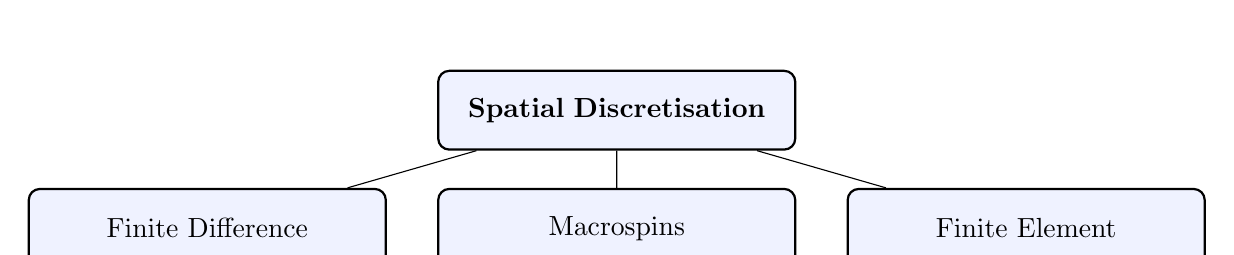
\begin{tikzpicture}[level 1/.style={sibling distance=5.2cm},level 2/.style={sibling distance=5cm}]
    \node[block] {\textbf{Spatial Discretisation}}
    child {node[block] {Finite Difference}}
    child {node[block] {Macrospins}}
    child {node[block] {Finite Element}};
  \end{tikzpicture}
  \caption{Spatial discretisation schemes used in micromagnetic models.}
  \label{fig:types-spat-discl}
\end{figure}


\subsubsection{Finite Difference Methods}
\label{sec:sd-finite-diff-meth}

Another method of spatial discretisation is the finite difference method: a single magnetisation vector is assigned to each point on (or ``cell'' in) a simple square/cubic grid which covers the system being modelled. The method is described in more detail in Section~\ref{sec:intr-finite-ele-diff}.

The finite difference method works well for very simple geometries when the grid can be lined up with all geometric features. For example when we are interested in comparing how different initial states evolve over time in a non-granular cuboid shaped piece of material a finite difference method will be sufficient (e.g. in the $\mu$mag standard problems\cite{mumag-website}). However for arbitrarily shaped grains, bit patterned media or any other more complex geometric system other methods are better suited.

NIST's \texttt{OOMMF} model, one of the oldest micromagnetic models still in use, uses the finite difference method\cite{oommf-website}.

\subsubsection{Finite Element Methods}
\label{sec:sd-finite-elem-meth}

A more complex method of spatial discretisation is the finite element method. Here the magnetic body is divided up into a finite number of polygonal \emph{elements} which can vary in size and shape. The points where these elements meet, known as the \emph{nodes}, are each assigned a magnetisation vector. Values at any other point in the domain can be calculated by interpolation between the nodes. More details of the method are given in Section~\ref{sec:intr-finite-ele-diff}.

The main advantage of the finite element method is that it can accurately approximate any geometrical feature by an appropriate arrangement of the polygonal elements.

The accuracy of the approximation will often depend on the size of the elements used and this can be varied arbitrarily as needed to give better accuracy in harder to model regions. The choice of element size can be done automatically using \emph{adaptive mesh refinement}: after each calculation an \emph{a posteriori} error estimate is calculated. If the error is determined to be too high anywhere the mesh is refined near that region and the calculation is repeated. Hence, given the desired error and a way of estimating the error, an appropriate mesh is automatically generated.\cite{Schrefl1999}

A downside is that the underlying maths can be more complex than that of the finite difference or macrospin models, hence increasing the time required to develop the model. Also the set up time can be greater because of the additional ``bookkeeping'' required.

Finite element methods are used in the \texttt{magpar}\cite{Scholz2003}, \texttt{nmag}\cite{Fischbacher2007} and \texttt{FEMME} micromagnetics models\cite{suessco-website}.

\subsection{Magnetostatic Field Calculations by Integral Methods}
\label{sec:magstat-field-calc-inte}

\begin{figure}[h]
  \centering
  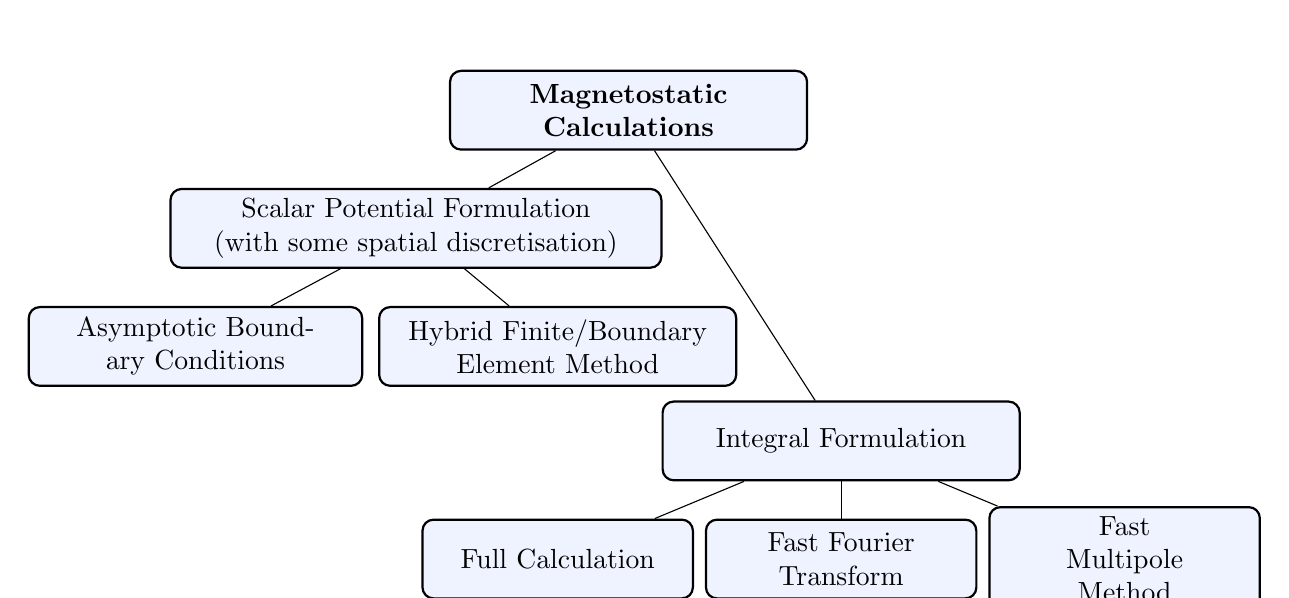
\begin{tikzpicture}[level 1/.style={sibling distance=5.4cm},
    level 2/.style={sibling distance=3.6cm}]

    \node[block] {\textbf{Magnetostatic Calculations}}
    child {node[block,text width=6cm] {Scalar Potential Formulation (with some spatial discretisation)}
      child{node[block,text width=4cm,xshift=-1cm] {Asymptotic Boundary Conditions}}
      child{node[block,text width=4.3cm] {Hybrid Finite/Boundary Element Method}}
    }
    child {node[block,yshift=-2.7cm] {Integral Formulation}
      child{node[block,text width=3.2cm] {Full Calculation}}
      child{node[block,text width=3.2cm] {Fast Fourier Transform}}
      child{node[block,text width=3.2cm] {Fast\\ Multipole\\ Method}}
    };
    \end{tikzpicture}
  \caption{Methods of magnetostatic field calculation that have been used in micromagnetic models.}
  \label{fig:types-mag-stat}
\end{figure}

The integral form of the magnetostatic field at a point $\xv \in \real^d$ due to the magnetic body $\magd$ with boundary $\boundd$ can be given in terms of magnetisation $\Mv$ by an integral over all volume and surface ``magnetic charges'' ($\nabla \cdot \Mv(\xv)$ and $\Mv(\xv) \cdot \nv(\xv)$ respectively) as
\begin{align}
  \Hms(\xv) &= \frac{1}{4 \pi} \Big[ - \int_\magd \frac{\big( \nabla' \cdot \Mv(\xv') \big)(\xv - \xv')}{| \xv -\xv'|^3} \d^3 \xv'
  + \int_\boundd \frac{ \big( \Mv(\xv') \cdot \nv(\xv') \big) (\xv - \xv')}{|\xv - \xv'|^3} \d^2 \xv' \Big],
  \label{eq:Hmsint}
\end{align}
where $\nabla'$ denotes the grad operator with respect to the $\xv'$ coordinate. For completeness we note that single magnetic charges (magnetic monopoles) have not been observed in nature. However they are a very useful mathematical tool for calculations of magnetic fields.

% Alternatively it can be given in terms of a sum over the dipole fields of magnetic moments (i.e. discretised magnetisation) as
% \begin{equation}
%   \label{eq:9}
%   \Hms(\xv) = \frac{1}{4\pi} \sum_i \frac{1}{|\xv - \xv_i|^3} \Big[ \mu_i(\xv_i) - 3(\mu_i(\xv_i) \cdot \ruv_i ) \cdot \ruv_i \Big],
% \end{equation}
% where $\ruv_i$ is the unit vector pointing from $\xv_i$ to $\xv$.

After the application of a discretisation scheme the integrals in equation~\eqref{eq:Hmsint} become a sum over all nodes. The naive way to calculate the magnetostatic fields would then be to work through the list of nodes calculating the field at each of them. Then for each node a contribution from all other nodes needs to be calculated. Hence this results in an algorithm complexity that scales as $O(N^2)$ (where $N$ is the number of points used in the space discretisation) which is usually unacceptably slow.

\subsubsection{Fast Fourier Transform Methods}

If the individual magnetic charges are on a regular lattice (or approximated by a regular lattice) and the boundary conditions are periodic, then the redundancy can be exploited to speed up the magnetostatic field calculations. The calculation of $\Hms$ in equation~\eqref{eq:Hmsint} can be thought of as applying a convolution operator $D$ (i.e. $\Hms = D \big[\Mv\big]$). The matrix corresponding to this operator  is only dependant on geometry, hence it can be precomputed, Fourier transformed and stored for use in the main simulation. Then all that is needed to calculate the magnetostatic field is to apply a Fourier transform to $\Mv$, compute the convolution and transform the result back into the time domain by applying the inverse Fourier transform. Because of the regularity, applying the convolution in the frequency domain is very fast and hence the complexity of the calculation is limited by the complexity of a fast Fourier transform, which is $O(N \log(N))$.\cite{Jones1997}

The downside of this method is that points to be calculated must be on a regular lattice, similar to the finite difference method. Hence, it is most suited for use in combination with models using a finite difference spatial discretisation. Alternatively it may be used in less regular macrospin models by approximating the the macrospins as being on a regular lattice.\cite{Jones1997}

A fast Fourier transform method is used to calculate the magnetostatic field in \texttt{OOMMF}.\cite{oommf-website}

\subsubsection{Fast Multipole Method}
\label{sec:fast-mult-meth}

An alternative method of calculation of the magnetostatic field is the multipole method. It takes advantage of the fact that distant magnetic charge has a much smaller effect on the total field at a point than nearby magnetic charge.

For the field calculation at a specific point, $\xv$, the full calculation is only performed for nearby magnetic charges. Groups of more distant charges are approximated (lumped) as a single multipole placed at the centre of the group. As the charges become more distant they contribute much less to the field due to the $\frac{1}{(\xv - \xv')^2}$ scaling in equation~\eqref{eq:Hmsint}. Hence for distant points the multipole approximation can become less accurate, and so faster to calculate, while still retaining the required overall level of accuracy.

The trick for quickly calculating fields at a large number of points is to pre-calculate the multipole approximations for a range of accuracies over all space. Then the calculation of a field at a single point only requires the full calculation of effects from a few nearby points and from the appropriate multipoles.\cite{Beatson}

One advantage of this method over the fast Fourier transform is that it allows for arbitrary geometries. Also the complexity of the method is $O(N)$, where $N$ is the number of magnetic charges (equivalent to the number of nodes/cells/macrospins after spatial discretisation).\cite{Chang2011}

The fast multipole method is used, with massive parallelisation for GPUs, to quickly calculate magnetostatic fields in FastMag.\cite{Chang2011} %??ds milan: how is load balencing performed?

\subsection{Magnetostatic Field Calculation by a Scalar Potential}
\label{sec:magstat-field-calc-pote}

When the magnetic field is being produced only by magnets and not currents (i.e. the magnetic field is irrotational) it is possible to express the field as a function of a scalar potential, $\phim$.\cite{Coey2010} Let $\magd$ be the magnetic body, $\boundd$ it's boundary and $\nv$ the outward unit normal on the boundary. Then we have
\begin{gather}
  \Hms = - \nabla \phim,  \label{eq:Hms} \\
  \nabla^2 \phim = \nabla \cdot \Mv \quad \xv \in \fulld, \label{eq:nnphim}
\end{gather}
With the following boundary conditions
\begin{gather}
  \phim^\inte - \phim^\exte = 0 \quad \xv \in \boundd, \label{eq:cont-phi-bound} \\
  \pd{\phim^\inte}{\nv} - \pd{\phim^\exte}{\nv} = \Mv \cdot \nv \quad \xv \in \boundd,
  \label{eq:nndphidn-bound} \\
  \phim \rightarrow 0 \text{ as } |\xv| \rightarrow \infty, \label{eq:phi-inf}
\end{gather}
where $\phim^\inte$/$\phim^\exte$ are the values of $\phim$ just inside/outside the domain, $\magd$.

This gives a formulation which can be solved using the finite element or finite difference discretisation methods. However, the zero boundary condition on $\phim$ at infinity, \eqref{eq:phi-inf}, is problematic. We obviously can not discretise an infinite domain to apply this condition since that would involve either infinite discrete elements or an infinitely sized element. Hence other techniques must be used.

The speed of the internal field calculation is given by the discretisation method, however applying the boundary conditions can require additional processing time.

% A third possibility is to define a vector potential $\vec{A}$ such that...

\subsubsection{Asymptotic Boundary Conditions}
\label{sec:asymptot-bcs}

One way to avoid an infinite domain is to truncate the external region at some finite distance from the magnetic domain. However the relationship between truncation distance and accuracy is problem dependant (since the size of the external field at any point depends on the problem geometry) and does not lead to good accuracy even for large truncation distances.

A more sophisticated method is to use asymptotic boundary conditions.\cite{Yang1997} The idea here is to use a truncated external region to calculate the boundary conditions on the magnetic domain that correspond to equation~\eqref{eq:phi-inf} being applied at infinity. Additionally the fact that any solution to the Poisson equation~\eqref{eq:nnphim} can be represented as an infinite series of harmonic functions is used to improve the accuracy. However the accuracy of this approach is still low compared to the hybrid method, even for large truncation distances.\cite{Bottauscio2008}

This method of applying the boundary conditions was used by Yang in GDM\cite{Yang1997} (general purpose dynamical micromagnetic code), but the code does not seem to be available any more.

\subsubsection{The Hybrid Boundary/Finite Element Method}
\label{sec:bound-elem-meth}

The idea of the hybrid method is to replace the external domain by a dipole layer placed on the surface of the magnetic domain which mimics the effect of the infinite external domain. This removes the need to truncate or discretise the infinite external domain. The full details of the method applied to magnetostatic calculations is discussed in Section~\ref{sec:hybr-finit-elem}.

A comparison by Bottauscio\cite{Bottauscio2008} found that using the hybrid method was more accurate than applying asymptotic boundary conditions for a calculation of the time evolution of the magnetisation of a sphere with zero exchange coupling. Even with a truncation distance of four times the size of the magnetic sphere (the total domain was $4^d$ times larger then the sphere) the accuracy when using asymptotic boundary conditions was worse and did not improve between truncation distances of three and four times the magnetic sphere radius. Even when exchange coupling was added (giving an easier test) the truncation method was worse than the hybrid element method.

One downside is an increase in the difficulty of creating the model since some parts of the boundary element method are mathematically different to the finite element method. For example singular integrals occur in the boundary element method and more advanced integration methods are needed. Also the hybrid method requires an additional dense matrix-vector multiplication for the calculation of boundary conditions.

The speed (and memory usage) of calculation of the boundary values in the method is limited by the dense matrix multiplication which is $O(N_b^2)$, where $N_b$ is the number of boundary nodes. The use of hierarchical matrix techniques can reduce this to $O(N_b \log(N_b))$.\cite{Knittel2009} Hence the speed of the hybrid method depends on the geometry. For example in 3D structures which are roughly spherical $N_b = O(N^{2/3})$ which gives optimal computation speed\footnote{With hierarchical matrix techniques the speed is $O(N^{2/3}\log(N^{2/3}))$ but $\log(x) << x^{1/2}$ for large $x$, hence $O(N^{2/3}\log(N^{2/3})) << O(N)$, i.e. optimal computation speed scaling.} but for extremely flat structures it can be as bad as $N_b = O(N)$.

The hybrid method was first applied to the computation of magnetostatic fields by Fredkin and Koehler.\cite{Fredkin1990}


\subsection{Time Discretisation}
\label{sec:time-discretisation}

After applying a spatial discretisation,we obtain a semi-discrete version of  equation~\eqref{eq:LLG}: it gives a continuous value in time of $\dMdt$ at fixed discrete points in space. To make it fully discrete, so that we can numerically solve for the time evolution of $\Mv$, we need to apply a time discretisation scheme. This section only relates to dynamic micromagnetics since energy based methods do not include time dependence.

The time discretisation methods discussed here all bear a strong similarity to the finite difference method discussed in Section~\ref{sec:finite-diff-appr}, except that the independent variable is time instead of space.

To explain the different time discretisation schemes we use a simple ordinary differential equation (an initial value problem)
\begin{align}
  \frac{dy}{dt} &= f(t,y(t)), \quad t \in [0,T],  \notag \\
  y(0) &= y_0.
  \label{eq:45}
\end{align}
where $f(t,y)$ is a known function and $T$ is the end time. The idea is to use the known values of $y(t)$ at the current/previous times along with the derivative to approximate the value $y(t+h)$  after stepping forwards in time by $h$.

Some key attributes of a time discretisation scheme are:\cite{Atkinson2009}
\begin{itemize}

\item \textbf{Stability} -- A scheme is stable if the approximated solution stays close to the exact solution, even after a large number of time-steps. A scheme is called conditionally stable if it is stable only for time-steps smaller than some maximum time-step or unconditionally stable if it is stable even for very large time-steps (although for very large time-steps the accuracy may be compromised).

\item \textbf{Convergence speed} -- An estimate of how rapidly the local truncation error decreases as the time-step, $h$, is reduced.

\item \textbf{Ability to deal with stiffness} -- Some ODEs have terms which vary on very different time scales, this is referred to as stiffness. Stiff ODEs causes some solvers to require extremely small time-steps in order to remain stable. The Landau--Lifshitz--Gilbert equation is sometimes stiff because the precession and damping terms usually operate on very different timescales but are both important for determination of the dynamics.\cite{Fidler2000}

\item \textbf{Preservation of geometrical properties} -- Some differential equations have properties which should ideally be conserved in the discretised system. For example $|\Mv|$ should remain constant over time in the Landau--Lifshitz--Gilbert equation but this property is often lost after discretisation.\cite{DAquino2005}

\item \textbf{Self-starting} -- A scheme is self starting if it only requires a single initial value. This is desirable because methods of estimating additional initial values may introduce errors. However more advanced schemes often require values at multiple times and so need multiple initial values.
\end{itemize}

\begin{figure}[h]
  \centering
  \resizebox{\textwidth}{!}{
    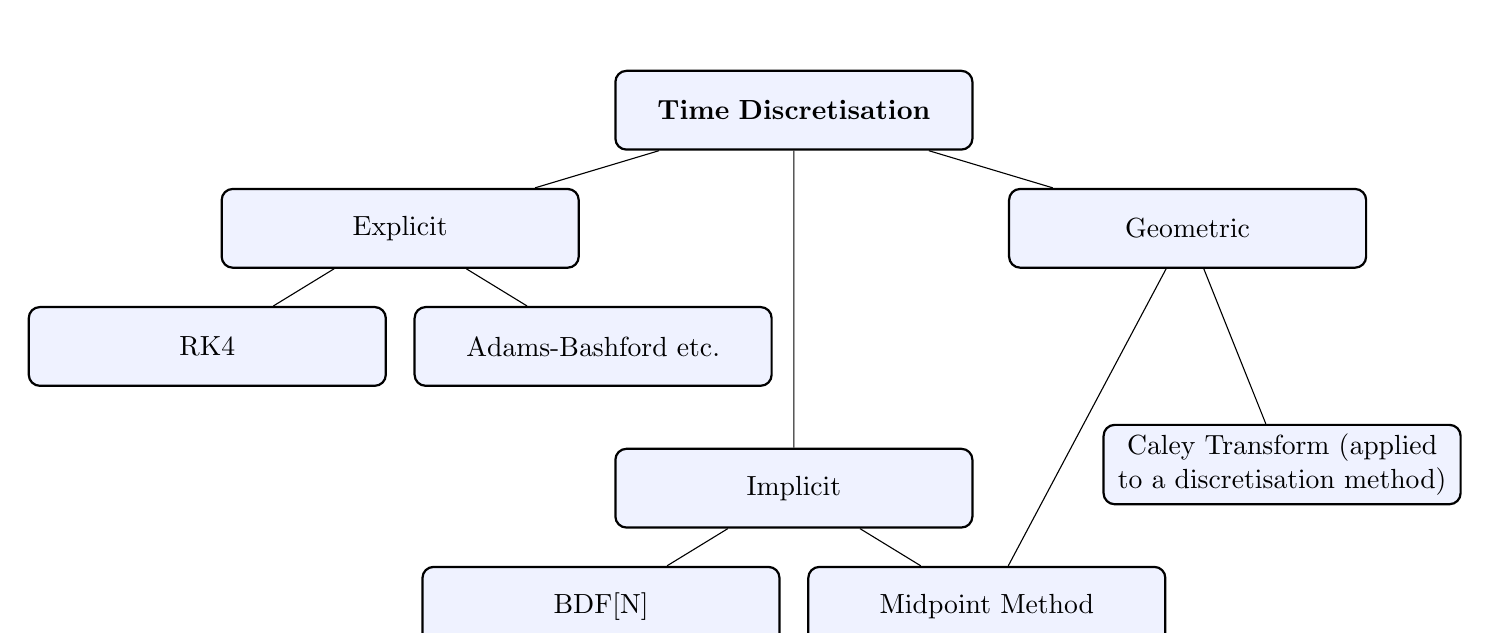
\begin{tikzpicture}[level 1/.style={sibling distance=5cm},level 2/.style={sibling distance=4.9cm},level 3/.style={sibling distance=4cm}]
      \node[block] {\textbf{Time Discretisation}}
      child{node[block] {Explicit}
        child{node[block] {RK4}}
        child{node[block] {Adams-Bashford etc.}}
      }
      child{node[block,yshift=-3.3cm] {Implicit}
        child{node[block] {BDF[N]}}
        child{node[block] (midpm) {Midpoint Method}}
      }
      child{node[block] (geom) {Geometric}
        child{node[block,xshift=1.2cm,yshift=-1.5cm] {Caley Transform (applied to a discretisation method)}}
      };
      \draw[line] (geom) -- (midpm);
    \end{tikzpicture}
  }
  \caption{Some time discretisation methods  used in micromagnetics.}
  \label{fig:types-time-disc}
\end{figure}

\subsubsection{Explicit Schemes}
\label{sec:explicit-schemes}

Explicit time discretisation schemes give the value at some future time in terms of the value at the present time and/or previous times. The simplest such scheme is the (forward) Euler method
\begin{equation}
  \label{eq:44}
  y(t_{n+1}) = y(t_n) + h f(t_n,y(t_n)),
\end{equation}
where $h$ is the time-step. Clearly, given $f(t,y)$ and an initial value for $y(t_0)$ we can solve for $y(t_n)$ for any $n$. However the stability and convergence behaviour of this simple scheme is less than impressive. Typically more advanced explicit schemes are used which give increased stability.\cite{Atkinson2009} Also the so called ``CFL condition'' (Courant-Freidrich-Lewy condition) can force the use of lower time-steps in explicit solvers if a finite element/difference spatial discretisation with small elements/cells is used.

Micromagnetics solvers for non-stiff systems commonly use the RK4 (fourth order Runge-Katta) method.\cite{Suess2002}


\subsubsection{Implicit Schemes}
\label{sec:implicit-schemes}

Implicit time discretisation schemes allow much longer time-steps to be used without loss of stability. However an implicit scheme gives the value at the next time-step in terms of current/previous times and in terms of the \emph{value at the next time-step}. Hence at each step a (linear or non-linear) system of equations must be solved, however the increase in maximum time-step size offsets this increase in calculation time per step in many cases.

The backwards differences schemes are a simple and commonly used example. The first order BDF formula is
\begin{equation}
  \label{eq:48}
  y(t_{n+1}) = y(t_n) + hf(t_{n+1}, y(t_{n+1})).
\end{equation}

Because a system of equations must be solved at each step a \emph{preconditioner} may be needed to ensure the system can be solved in optimal time (i.e. $O(N)$). Magnetostatic field calculation by the hybrid method can cause difficulties in the solution of the system of equations because it adds a dense sub-block to the otherwise sparse system.

Micromagnetics models commonly use BDF schemes of various order\cite{Suess2002} for the modelling of stiff systems. The midpoint method is another possible choice.\cite{DAquino2005}

Other micromagnetic models use a combination of implicit and explicit schemes: everything except for the magnetostatic field is discretised as normal using an implicit scheme, the magnetostatic field is updated (using an explicit calculation) after each time step. This method gains a larger time-step from the implicit method but the system of equations to be solved remains sparse. However when using this method the determination of the time-step must be done specially (i.e. not using normal adaptivity) since the system of equations contains no information on the magnetostatic field.\cite{Schrefl1997}

\subsubsection{Adaptivity}
\label{sec:adaptivity}

Adaptive time discretisation methods vary the time-step in response to an estimate of the local truncation error. This is especially computationally efficient when the magnitude of the time derivative varies widely over time, for example if the magnetisation direction changes slowly until some unknown time when it rapidly switches.

\subsubsection{The Non-Convex Constraint}
\label{sec:ensuring-constant-mv}

Note that in equations~\eqref{eq:LL}, \eqref{eq:Gilbert} and \eqref{eq:LLG} the direction of $\dMdt$ is always perpendicular to the current value of $\Mv$ (since all terms contain cross products with $\Mv$). Hence we have an implicit condition: $|\Mv| = M_s$. However in the discretised approximation this is often lost and must be enforced separately. This condition is often called a  \emph{non-convex constraint}\footnote{Intuitively a convex set is one such that given two members of the set all points on a straight line between them are also members of the set. With the condition $|\Mv|=M_s$ the set of possible values of $\Mv$ is the surface of a sphere with radius $M_s$ which is not a convex set, hence the name.}. This can pose difficulties in the numerical solution of the Landau--Lifshitz--Gilbert equations because the approximations used do not necessarily respect the constraint. Hence the solution can end up with $|\Mv| \neq M_s$ which is un-physical (for constant temperature models).

A simple method of dealing with the constraint is to re-normalise $\Mv$ after some number of time-steps or when the error in $|\Mv|$ exceeds some tolerance.\cite{Fidler2000} However this approach fundamentally changes the system of equations being solved.\cite{Lewis2003}

If we have a system with only a single (macro)spin (i.e. a single value of $\Mv$ represents the magnetisation of the entire system) it is easy to avoid this problem by using a spherical polar coordinate system $(r,\theta,\phi)$. Equation~\eqref{eq:LLG} can be expressed in terms of only the angles $(\theta,\phi)$ representing the direction of $\Mv$ and the non-convex constraint is automatically enforced since
\begin{equation}
  \label{eq:40}
  \pd{|\Mv|}{t} = \pd{r}{t} \equiv 0.
\end{equation}
However to extend this to systems where $\Mv$ varies with space we have to use a separate spherical polar coordinate system at each point where $\dMdt$ is calculated. Also a Cartesian global coordinate system is still needed to calculate the interactions between the discretised points (i.e. magnetostatics, exchange coupling). Hence we have to convert back and forth between coordinate systems during the simulation.\cite{Scholz2003} Finally problems can occur with this approach as the polar angle, $\theta$, approaches zero because $\pd{\Mv}{t} \propto \frac{1}{\sin(\theta)}$.\cite{Fukushima2005}

% Some people have used special test functions to keep $|\Mv|$ fixed, don't understand that method yet though

``Geometrical'' integration schemes aim to solve this problem by constructing a time discretisation scheme that naturally preserves the value of $|M_s|$. An example of such a scheme is the midpoint method as used by d'Aquino. The midpoint method also has other desirable properties -- it conserves energy when the damping term is zero and it ensures that the energy is a decreasing function of time when the damping is non-zero.\cite{DAquino2005} Alternatively geometrical integration methods based on Cayley transforms can be used.\cite{Lewis2003}\cite{Bottauscio2011}
% ??ds however the proofs do not work for a weak formulation...


% \subsubsection{Preconditioning}

% \begin{itemize}
% \item If implicit time-stepping is used solution of the linear systems created at each time-step can be troublesome.
% \item We can speed this up using a preconditioner.
% \item Some work has been done on preconditioning by Suess et. al. \cite{Suess2002}.
% \item Also Banas et. al.\cite{Banas2008} \cite{Banas2010} used a multigrid preconditioner for the Maxwell-LLG equation( magnetostatic field is computed via Maxwell's equations, exchange field is also accounted for, crystalline anisotropy is not). The use of Maxwell's equations introduces complications because of the curls.
% \end{itemize}

\subsubsection{Specific micromagnetics time discretisation schemes}

??ds write something about the work summarised in Cimrak's review.

\subsection{Conclusions}
\label{sec:model-conclusions}

A dynamic modelling method will be used because the ability to model time dependant processes is essential.

For the spatial discretisation a macrospin model is not considered because its application is limited to cases with well separated grains and because it is not able to model effects inside a grain. Therefore a finite element spatial discretisation will be used because the ability to treat arbitrary geometries is extremely desirable (for example in the modelling of bit patterned media). Additionally \texttt{oomph-lib}\cite{oomph-lib-website} (a multi-physics open source finite element modelling library) gives an excellent framework in which to construct a new finite element micromagnetic model. This choice will also allow easy extension to the modelling of heat assisted magnetic recording using a finite element discretisation of the heat equation to model heat flow.

The magnetostatic field will be evaluated from a scalar potential by the hybrid finite/boundary element method. A finite element method will be used because it can be easily integrated into the overall model. The hybrid method will be used to apply boundary conditions because the accuracy loss involved in efficiently approximating the external region by asymptotic boundary conditions is large and problem dependant.

The time discretisation scheme used will be the mid-point method because of it's preservation of magnetisation vector length and ability to deal with stiffness. The use of preconditioners to speed up to the solution of the non-linear system created at each time-step will be investigated.

%%% Local Variables:
%%% mode: latex
%%% TeX-master: "main"
%%% End:


\section{Introduction to Finite Difference and Finite Element Approximations}
\label{sec:intr-finite-ele-diff}

The finite difference and finite element methods allow the \emph{discretisation} of a continuous differential equation to allow for solution by computational methods. The finite element method allows for more complex geometries than the finite difference method, at the cost of increased complexity and setup time.

A simple problem is used to illustrate these methods: solving the Poisson
equation in one spatial dimension. Find\footnote{A function $g\in C^{k}(0,1)$ if $g$ and it's first $k$ derivatives are continuous on $(0,1)$.} $y(x)\in C^{2}(0,1)$ such that
\begin{equation}
  -y''=f\qquad\text{on }(0,1)
  \label{eq:poisson1}
\end{equation}
\begin{equation*}
  y(0)=y_{a},\quad y(1)=y_{b},\quad f=f(x)\in C(0,1).
\end{equation*}

\subsection{Finite Difference Approximation}
\label{sec:finite-diff-appr}

We start with the equation~\eqref{eq:poisson1} and subdivide this interval into
$N$ sub intervals each of length $h = \frac{1}{N}$ as shown in Figure
\ref{fig:The-subdivision}. The points $x_{i}$ are the points where we will
approximate $y(x)$ (\ie we will compute a discrete solution $y(x_{i})$ for
$i=0, \, \ldots \, ,N$).

\begin{figure}[!ht]
  \center
  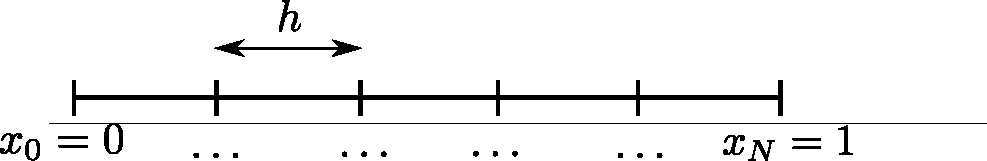
\includegraphics[width=1\textwidth]{./images/finite_diff_discretisation}
  \caption{Subdivision of the unit interval for finite difference approximation.}
  \label{fig:The-subdivision}
\end{figure}

The Taylor series for a function $y(x)$ at a point $x$ near $a$
is defined as
\begin{equation*}
  y(x)=y(a)+y'(a)(x-a)+\dfrac{y''(a)}{2!}(x-a)^{2}
  + \dfrac{y'''(a)}{3!}(x-a)^{3}+\dfrac{y^{(4)}(a)}{4!}(x-a)^{4}\ldots.
\end{equation*}

Using $a=x_{i}$ and $x=x_{i+1}$ we get
\begin{equation}
  y(x_{i+1})=y(x_{i})+hy'(x_{i})+\dfrac{h^{2}}{2}y''(x_{i})+\dfrac{h^{3}}{3!}y'''(a)+O(h^{4}),
  \label{eq:taylor1}
\end{equation}
where $O(h^{4})$ is the residual. Similarly for $x=x_{i-1}$
\begin{equation}
  y(x_{i-1})=y(x_{i})-hy'(x_{i})+\dfrac{h^{2}}{2}y''(x_{i})-\dfrac{h^{3}}{3!}y'''(a)+O(h^{4}).
  \label{eq:taylor2}
\end{equation}

Adding equations~\eqref{eq:taylor1} and \eqref{eq:taylor2} gives
\begin{equation*}
  y(x_{i+1})+y(x_{i-1})=2y(x_{i})+h^{2}y''(x_{i})+O(h^{4}).
\end{equation*}
We then rearrange to get an expression for $y''(x_{i})$ in terms of $y$:
\begin{equation*}
  y''(x_{i})=\dfrac{1}{h^{2}}\Big[y(x_{i+1})+y(x_{i-1})-2y(x_{i})\Big]+O(h^{4}).
  % Milan says error is O(h^{4}) but I can't see why it's not O(h^{2})...
\end{equation*}

We now drop the $O(h^{4})$ term leaving an approximation for $y''(x_{i})$
\begin{equation}
  y''(x_{i})=\dfrac{1}{h^{2}}\Big[y(x_{i+1})+y(x_{i-1})-2y(x_{i})\Big],
  \label{eq:y''approx}
\end{equation}

with an error of order $h^{4}$ (so the error rapidly decreases with small
sub intervals). Similar manipulation of the Taylor series can be used to obtain
other derivatives of $y$ for use when solving differential equations other than
the Poisson equation. For example $y'$ can be found by subtracting equation
\eqref{eq:taylor2} from equation~\eqref{eq:taylor1}.

Substituting the approximations for $y''(x_{i})$ from equation~\eqref{eq:y''approx}
into \eqref{eq:poisson1} at each $x_{i}$ gives a set of $n$ linear
equations for the unknowns $y(x_i) = y_i \, (i=1 , \, \ldots \, , n)$

\begin{equation*}
  \dfrac{1}{h^{2}}\Big[y(x_{i+1})-2y(x_{i})+y(x_{i-1})\Big]=-f(x_{i}).
\end{equation*}

We introduce a shorthand notation often used in this area: $y_{i}=y_{h}(x_{i})$
and $f_{i}=f(x_{i})$. Multiplying by $-1$ and changing to the new
notation gives
\begin{equation}
  \dfrac{1}{h^{2}}\Big[-y_{i+1}+2y_{i}-y_{i-1}\Big]=f_{i}.
  \label{eq:23}
\end{equation}

So far we have not included the boundary conditions in \eqref{eq:23}. We know
from the problem specification that $y(x_{0})=y_{a}$ and $y(x_{n+1})=y_{b}$.  A
simple way to enforce these conditions is to include them as two additional
trivial equations in our linear system. For example the linear system
approximating the Poisson equation at three points (since $y(x_{0})$ and
$y(x_{4})$ are known) is then:

\begin{equation*}
  \dfrac{1}{h^{2}}\left[
    \begin{array}{ccccc}
      h^{2} & 0 & 0 & 0 & 0\\
      -1 & 2 & -1 & 0 & 0\\
      0 & -1 & 2 & -1 & 0\\
      0 & 0 & -1 & 2 & -1\\
      0 & 0 & 0 & 0 & h^{2}
    \end{array}
  \right]\left[
    \begin{array}{c}
      y_{0}\\ y_{1}\\ y_{2}\\ y_{3}\\ y_{4}
    \end{array}
  \right]  =  \left[
    \begin{array}{c}
      y_{a}\\ f_{1}\\ f_{2}\\ f_{3}\\ y_{b}
    \end{array}
  \right],
\end{equation*}

which simplifies to

\begin{equation}
  \dfrac{1}{h^{2}}\left[
    \begin{array}{ccc}
      2 & -1 & 0\\
      -1 & 2 & -1\\
      0 & -1 & 2
    \end{array}
  \right]\left[
    \begin{array}{c}
      y_{1}\\ y_{2}\\ y_{3}
    \end{array}
  \right]=\left[
    \begin{array}{c}
      f_{1}+y_{a}/h^{2}\\ f_{2}\\ f_{3}+y_{b}/h^{2}
    \end{array}
  \right].
  \label{eq:simple-linear-eq-finite-diff-1}
\end{equation}

This can be easily solved computationally by using standard linear algebra solvers.


\subsubsection{Example}

\begin{figure}[!ht]
  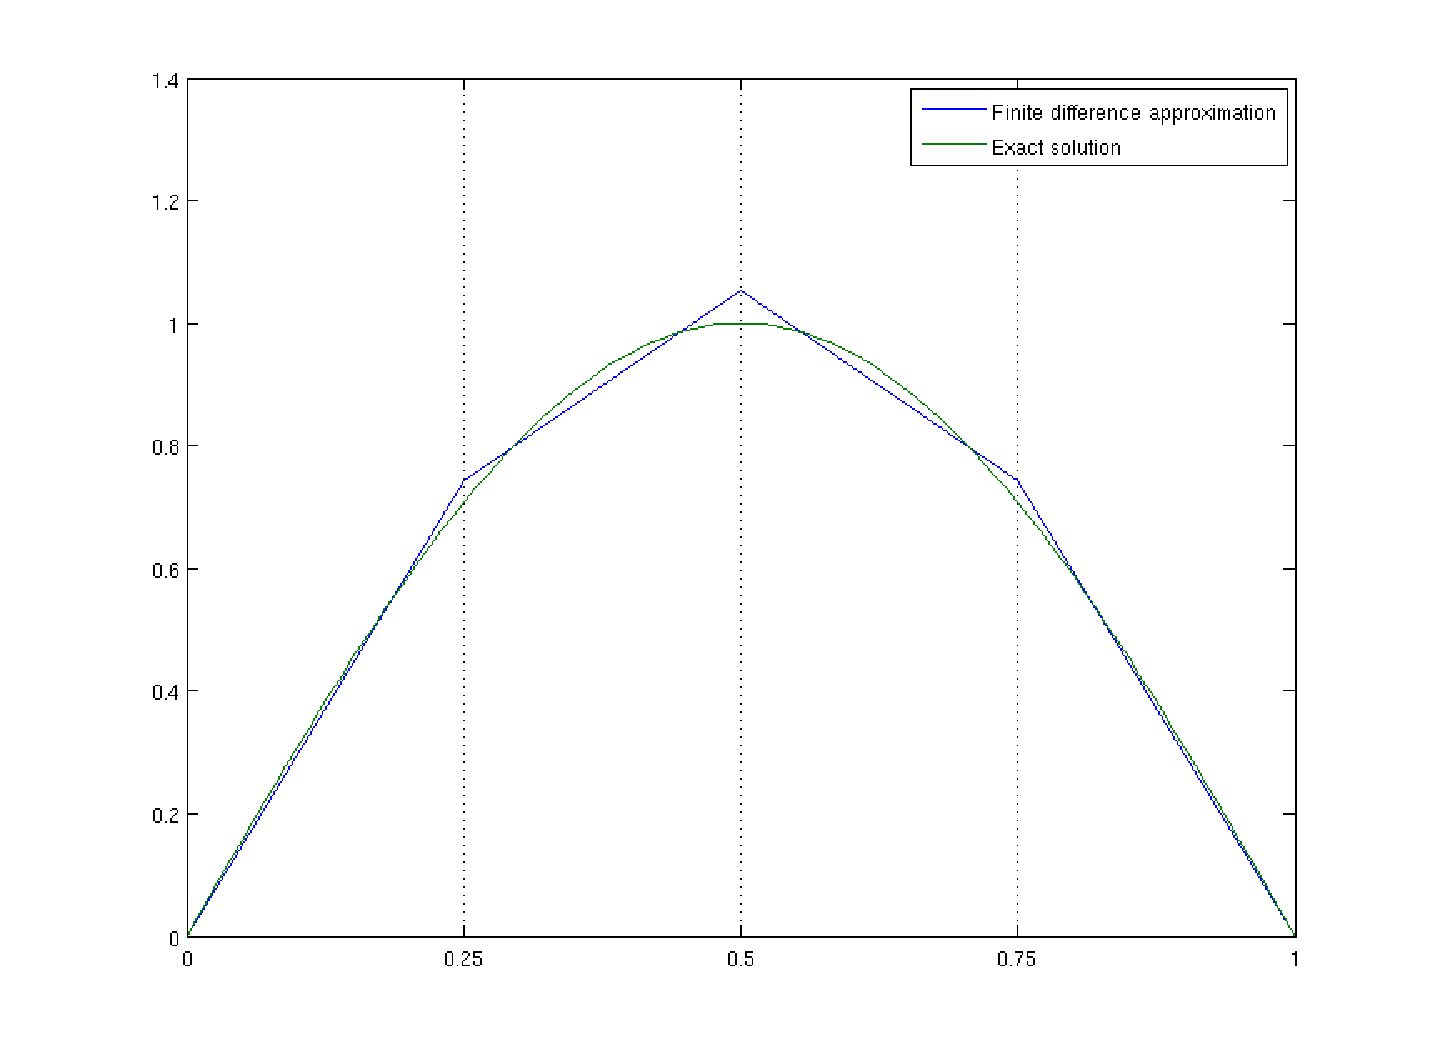
\includegraphics[width=1\textwidth]{./images/finitediffexample}
  \caption{A finite difference approximation for $y''(x)=-\pi^{2}\sin(\pi x)$,
    $y(0)=0$ and $y(1)=0$ for $x\in[0,1]$. The exact solution is $y(x)=\sin(\pi x)$.}
  \label{fig:A-finite-difference-example}
\end{figure}

We will use an $f(x)$ which corresponds to an exact solution. Let
$y(x)=\sin(\pi x)$, then $f(x)=\pi^{2}\sin(\pi x)$, $y(0)=0$ and
$y(1)=0$. Let $N=5$, then the linear system to be solved is:

\begin{equation*}
  \dfrac{1}{(0.25)^{2}}\left[
    \begin{array}{ccc}
      2 & -1 & 0\\
      -1 & 2 & -1\\
      0 & -1 & 2
    \end{array}
  \right]\left[
    \begin{array}{c}
      y_{1}\\ y_{2}\\ y_{3}
    \end{array}
  \right] = \left[
    \begin{array}{c}
      \dfrac{\pi^{2}}{\sqrt{2}}+0\\
      \pi^{2}\\
      \dfrac{\pi^{2}}{\sqrt{2}}+0
    \end{array}
  \right].
\end{equation*}

Solving for $\mathbf{y} = [ y_1, y_2, y_3]$ gives
\begin{equation*}
  \left[
    \begin{array}{c}
      y_{1}\\ y_{2}\\ y_{3}
    \end{array}
  \right]=\left[
    \begin{array}{c}
      0.74\\ 1.05\\ 0.74
    \end{array}
  \right],
\end{equation*}
which is plotted in Figure~\ref{fig:A-finite-difference-example}.


\subsection{Finite Elements}
\label{sec:finite-elements-one-d}

\subsubsection{Definitions}
\label{sec:fem-definitions}

The function space $L^{2}$ is the set of all functions $f(x)$ such
that $\intop_{-\infty}^{\infty}|f(x)|^{2}dx$ is finite.

The span of a set of functions is the set of all possible linear combinations of
the functions. If a set of functions $\{\phi_{i}\}$ is such that
$V=\text{span}(\phi_{i})$ then we say that $\{\phi_{i}\}$ spans $V$ and
$\{\phi_{i}\}$ is a basis for the function space $V$. If $V$ has a basis consisting of a finite number of functions then we say that $V$ is finite dimensional, otherwise $V$ is infinite dimensional.

In finite element models we are interested in approximating an infinite
dimensional space (the space of solutions) by a finite dimensional
space (the space of approximations).

The $n$-th Sobelov space is the space of all functions such that they and their $n$-th derivatives (in all dimensions) are in $L^2$. For example
\begin{equation}
  \label{eq:H1}
  \sob^1(\magd) = \{ y \st y, \pd{y}{x_i} \in L^2(\magd) \; \forall x_i \}
\end{equation}

\subsubsection{The Weak Formulation \& A Discretisation}
\label{Derivation-of-weighted-residuals}

The method of weighted residuals is a way to convert a differential equation
into an integral form that can be modelled computationally. As such it is the
first step in a variety of modelling methods including the finite element method
and the spectral method.

For simplicity we start, as before, with the one-dimensional Poisson equation
\eqref{eq:poisson1}, with homogeneous Dirichlet boundary conditions
(\ie $y_{a}=y_{b}=0$).

% \footnote{The functions must be Lipschitz continous (a stronger form
%   of continuity than standard). Lipschitz continuity is defined as the
%   following: for $X,Y$ metric spaces with metrics $d_{x}(x_{1},x_{2})$,
%   $d_{y}(y_{b},y_{2})$ respectively then a function $f:X\rightarrow Y$ is
%   Lipschitz continuous if and only if $\exists K\geq0$ s.t. $\forall
%   x_{1},x_{2}\in X$ $d_{y}(f(x_{1}),f(x_{2}))\leq K\, d_{x}(x_{1},x_{2})$.}

The formulation used in \eqref{eq:poisson1} is too restrictive for our purposes:
it disallows some useful approximating functions, and in higher dimensional
cases restricts the domain shapes that can be modelled
\cite{HowardElmanDavidSilvester2006}. However for well behaved functions the
following \emph{weak formulation} is equivalent: find $y\in V_{s}$ such that
\begin{equation}
  -\int_{0}^{1}y''v\, dx=\int_{0}^{1}fv\, dx \qquad \forall v\in V_{T}.
  \label{eq:26}
\end{equation}

Here $V_{T}$ is some appropriate space of \emph{test functions}. The test
functions must satisfy $V_{T}\subseteq \sob^0(0,1)$, in order to ensure that the integrals in \eqref{eq:26} are well defined. Thus
\begin{equation}
  \label{eq:28}
  V_{T}=\{v:[0,1]\rightarrow\mathbb{R}\, \st \, v \in \sob^0(0,1)\}.
\end{equation}

The space $V_{s}$ is the solution space
\begin{equation*}
  V_{s}=\{y:[0,1]\rightarrow\mathbb{R}\, \st \, y \in \sob^2(0,1),\,
  y(0) = y_{a},\, y(1) = y_{b}\},
\end{equation*}
 \ie the space of functions that are sufficiently smooth for the integrals to be finite and that satisfy the boundary conditions.

To see that the weak form is equivalent consider the case when the error or \emph{residual} $f(x) -y(x)''$ is non-zero for some $x \in [0,1]$. Since equation~\eqref{eq:26} must hold for all functions $v$ we can come up with a function which is non-zero at $x$ and hence the equality in \eqref{eq:26} fails. We call this the method of weighted residuals because we use a weighted integral of the residual to approximate the true equation.\cite{Zeinkiewicz1967}%pg 210,214

The smoothness restrictions on our weak form approximation can be further reduced using integration by parts
\begin{equation*}
  \int_{0}^{1}q\, dp=\Big[pq\Big]_{0}^{1}-\int_{0}^{1}p\, dq,
\end{equation*}
applied to the left hand side of equation~\eqref{eq:26}. Let $p=y'$ and $q=v$, then
\begin{equation}
  -\int_{0}^{1}y''v\, dx=-\Big[y'v\Big]_{0}^{1}+\int_{0}^{1}y'v'\, dx.
  \label{eq:29}
\end{equation}

We now introduce a second constraint to the test functions: $v=0$
at the boundaries (\ie $v_a=v_b=0$), so the bracketed term in \eqref{eq:29} is
zero and we are left with
\begin{equation*}
  -\int_{0}^{1}y''v\, dx=\int_{0}^{1}y'v'\, dx.
\end{equation*}

Hence our problem can be reduced to the following: find $y\in V_{S}'=\{y \st \, y \in \sob^1(0,1),\, y(0) = y_a, y(1) = y_b \}$
such that
\begin{equation}
  \int_{0}^{1}y'v'\, dx=\int_{0}^{1}fv\, dx\qquad\forall v\in V'_{T}=\{v \st \, v \in \sob^1(0,1),\, v_a=v_b=0\}.\label{eq:symmetric-weak-poisson}
\end{equation}

Note that this rearrangement has removed the second derivative in $y$, hence we only require $y \in \sob^1(0,1)$ instead of $y \in \sob^2(0,1)$. This allows a wider range of shape
functions to be used but comes at the expense of requiring more smoothness in
the test functions. Also note that if $y_a = y_b = 0$ then $V_{S}'=V_{T}'$, our
test and solution spaces are the same.

Equation~\eqref{eq:symmetric-weak-poisson} is still inapplicable as a
computational method since the test (and solution) space is infinite dimensional
(\ie the problem is still continuous). So for the next step we approximate
$V_{T}'$ by a finite dimensional function space $V_{T}^{h}\subset V_{T}'$ such
that
\begin{equation}
  V_{T}^{h}=\text{span} \{ \tbf_{\ndi} \}_{n=1}^{N}
  =  \{v_h \st v_h = \sum_{n=0}^{N}\alpha_{\ndi} \tbf_{\ndi},\, \alpha_{\ndi} \in \real,\, v_a = v_b =0 \},
  \label{eq:30}
\end{equation}
for some finite set of basis functions $\tbf_{\ndi}$. Similarly for $V_S$
\begin{equation}
  \label{eq:34}
    V_{S}^{h}=\text{span} \{ \sbf_{l} \}_{l=1}^{N_l}
    =  \{y_h \st y_h = \sum_{l=0}^{N_l}c_{l} \sbf_{l},\,
    c_{l} \in \real,\, y(0) = y_a,\, y(1) = y_b \}.
\end{equation}

We call $\sbf_l$ the \emph{shape functions}. The choice of $\tbf_{\ndi}$
and $\sbf_l$ lead to different modelling methods, the choice corresponding
to the finite element method will be discussed in section \ref{sub:Actual-Finite-Elements}. For now we convert the problem into a general discrete form.

We currently have the \emph{discrete weak formulation} of \eqref{eq:poisson1}: find $y_{h}\in V_{S}^{h}$ such that
\begin{equation}
  \int_{0}^{1}y'_{h}v_{h}'\, dx=\int_{0}^{1}fv_{h}\, dx\qquad\forall v_{h}\in V_{T}^{h}.
  \label{eq:discrete-weak-prob}
\end{equation}

Replacing $v_{h}$ from \eqref{eq:discrete-weak-prob} by $\tbf_{\ndi}$
gives
\begin{equation}
  \int_{0}^{1} y'_{h} \tbf_{\ndi}' \, dx = \int_{0}^{1}f\tbf_{\ndi}\, dx\qquad n=0,\ldots,N,
  \label{eq:discrete_weak_test_fns_replaced}
\end{equation}

Since $y_{h}\in V_{S}^{h}$ we can also replace $y_{h}$ by a linear combination
of the spanning functions, \ie
\begin{equation}
  y_{h}=\sum_{l=0}^{N_l}c_{l}\sbf_{l},
  \label{eq:y-spans}
\end{equation}
where $c_l \in \real$ are the (unknown) coefficients.

Substituting \eqref{eq:y-spans} into equation~\eqref{eq:discrete_weak_test_fns_replaced} gives
\begin{equation}
  \sum_{l=0}^{N_l}c_{l}\int_{0}^{1}\sbf_{l}'\tbf'_{\ndi}\, dx=\int_{0}^{1}f\tbf_{\ndi}\, dx
  \qquad n=0,\ldots,N.
  \label{eq:31}
\end{equation}

The functions $f$, $\tbf$ and $\sbf$ are known and so the integrals in \eqref{eq:31} are just numbers (which must be explicitly calculated at some point). Hence we introduce a matrix $A$ and a vector $\mathbf{b}$ containing these numbers:
\begin{equation}
  \int_{0}^{1}\sbf_{l}'\tbf'_{\ndi}\, dx=A_{l\ndi},\qquad\int_{0}^{1}f\tbf_{\ndi}\, dx=b_{j},\label{eq:Aij_bj}
\end{equation}
and the problem is reduced to a system of linear equations
\begin{equation}
  A\mathbf{c} = \mathbf{b}.
  \label{eq:final_galerkin}
\end{equation}
This can be solved to find the vector of unknown coefficients $\mathbf{c}$ which can be substituted into \eqref{eq:y-spans} to give an approximation for $y$.


\subsubsection{Finite Elements in One Dimension}
\label{sub:Actual-Finite-Elements}

To create a useable implementation of the methodology derived in Section~\ref{Derivation-of-weighted-residuals} we must first define a set of basis functions $\tbf_\ndi$ for the space $V_{T}^{h}$ and a set of $\sbf_l$ for the space $V_S^h$. For simplicity we choose the two types of basis functions to be the same: $\sbf_l = \tbf_l$. This choice defines the Galerkin method (and often results in symmetric matrix $A$).\cite{Zeinkiewicz1967} %pg215


The overall aim is to approximate an arbitrary function at a finite set of \emph{nodes}, $x_\ndi$, by a linear combination of a finite set of simple functions, $\tbf_\ndi$. There are a variety of useful choices for $\tbf_\ndi$ but we will focus on a carefully constructed set of polynomials -- the Lagrange interpolation basis functions, defined as
\begin{equation*}
  L_\ndi(x)=\prod_{k\neq i}\Bigg(\dfrac{x-x_{k}}{x_\ndi-x_{k}}\Bigg).
\end{equation*}

This definition results in the following useful properties of $L_{\ndi}(x)$
\begin{equation}
  \label{eq:35}
  L_{\ndi}(x_{\ndi}) =
  \begin{cases}
    1 & k = \ndi, \\
    0 & k \neq \ndi,
  \end{cases}
\end{equation}
since at each $x_{\ndi}$ with $k \neq \ndi$ one of the numerators is zero and at
$x_{\ndi}$ all of the numerators are equal to the corresponding denominator.

Polynomials are chosen because they are easy to manipulate computationally, for example differentiation and integration are simple. Also an arbitrary level of accuracy can be achieved when approximating the a smooth function by piecewise polynomials, provided that the polynomials are only non-zero on a sufficiently small area (\ie after sufficient mesh refinement).

We now consider the simple case where we approximate the function at two points
$x_{0}$ and $x_{1}$ (linear interpolation). Then the Lagrange basis
functions are simply
\begin{equation}
  L_{0}=\dfrac{x-x_{1}}{x_{0}-x_{1}},\qquad
  L_{1}=\dfrac{x-x_{0}}{x_{1}-x_{0}}.
  \label{eq:simple_lagrange}
\end{equation}
The interpolation of a function on the interval $[x_{0},x_{1}]$ is then given by
\begin{equation*}
  y_{h}(x)=y(x_{0})L_{0}(x)+y(x_{1})L_{1}(x).
\end{equation*}

It is advantageous to work with such simple functions even for very complex
models because evaluation of integrals and interpolation is quick and easy. We
can achieve this by splitting the domain into a set of $N$ \emph{elements}
$e_{0},e_{1},\ldots,e_{N-1}$, which can be of varying size (in contrast to the
basic finite difference method where the nodes had to be equally spaced). We
then create a \emph{local} numbering scheme for the nodes and functions in each
element and a \emph{global} numbering scheme to keep track of the same nodes and
functions over the entire domain.

In one dimension the boundary of each element consists of two points, one at
each end. In the local scheme it is natural to label these points by the element
number $e$ and a local node number, \ie $x_{0}^{(e)}$ and $x_{1}^{(e)}$. In the
global scheme each node is labelled by a unique node number, \ie $x_{\ndi}$ for
$\ndi=0,\ldots,N$. The concept is best illustrated by a diagram, see Figure
\ref{fig:local-global-numbering}.

\begin{figure}[ht]
  \center
  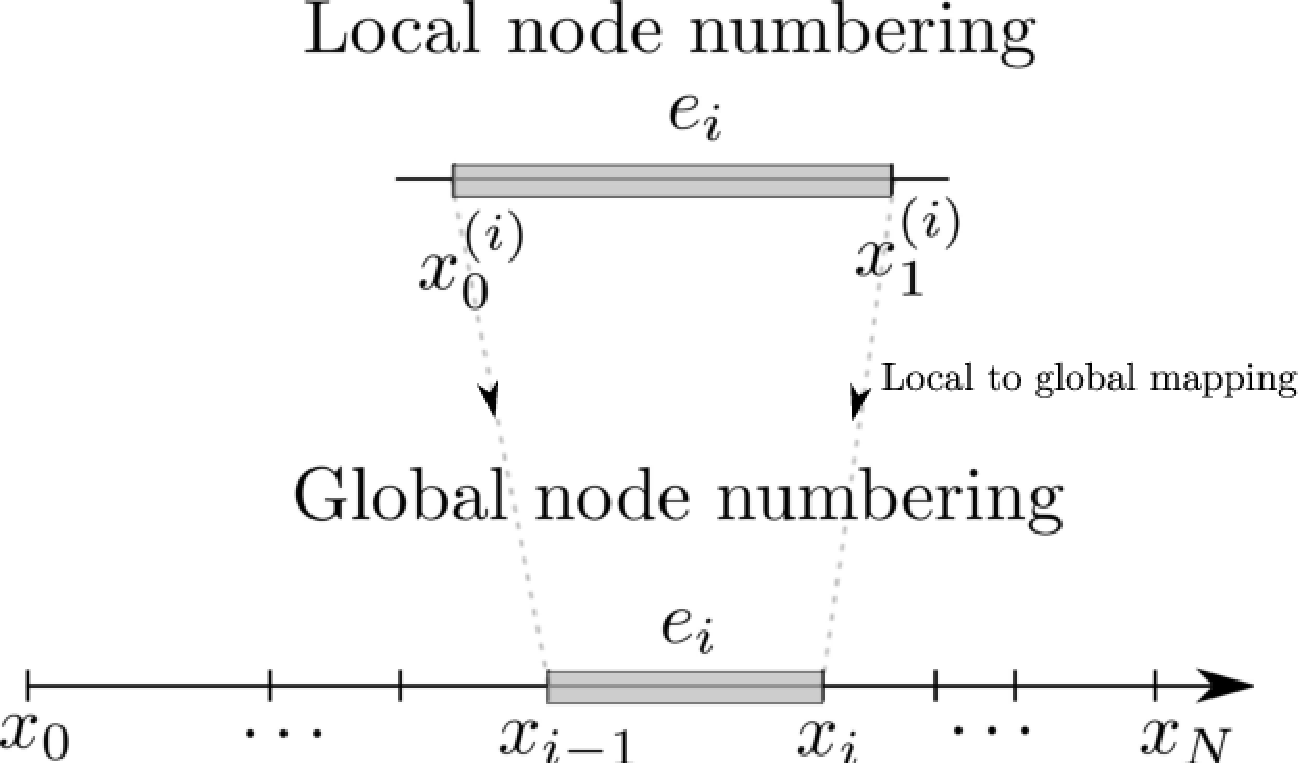
\includegraphics[width=0.8\textwidth]{./images/local_global_numbering}
  \caption{The local and global numbering schemes for nodes in a one-dimensional
    finite element model.}
  \label{fig:local-global-numbering}
\end{figure}

The process of assigning a global node number to each local node is known as the
local to global mapping. Good book keeping of the mapping is essential,
especially in higher dimensions when this it becomes much more complex.

We define the local basis functions in element $e$ as
\begin{equation}
  L_{0}^{(e)}(x)=\dfrac{x-x_{1}^{(e)}}{x_{0}^{(e)}-x_{1}^{(e)}},\qquad
  L_{1}^{(e)}(x)=\dfrac{x-x_{0}^{(e)}}{x_{1}^{(e)}-x_{0}^{(e)}}
  \qquad\text{for }x\in e=[x_{0}^{(e)},x_{1}^{(e)}].
  \label{eq:32}
\end{equation}
Except for the test functions when $\ndi$ is a boundary node. In this case we define $L_\ndi^{(e)} = 0$.
The $\ndi$th global basis function is then defined as:
\begin{equation}
  \label{eq:33}
  L_\ndi(x) =
  \begin{cases}
    L_\ndi^{(e)}(x) & \text{if node $\ndi$ is in element $e$,} \\
    0 & \text{otherwise.}
  \end{cases}
\end{equation}

\begin{figure}[!ht]
  \center
  % ??ds numbering: change e_i to element e, e_{i+1} to e+1, x_i to x_\ndi, x^(i) to x^(e) L_i to L_\ndi
  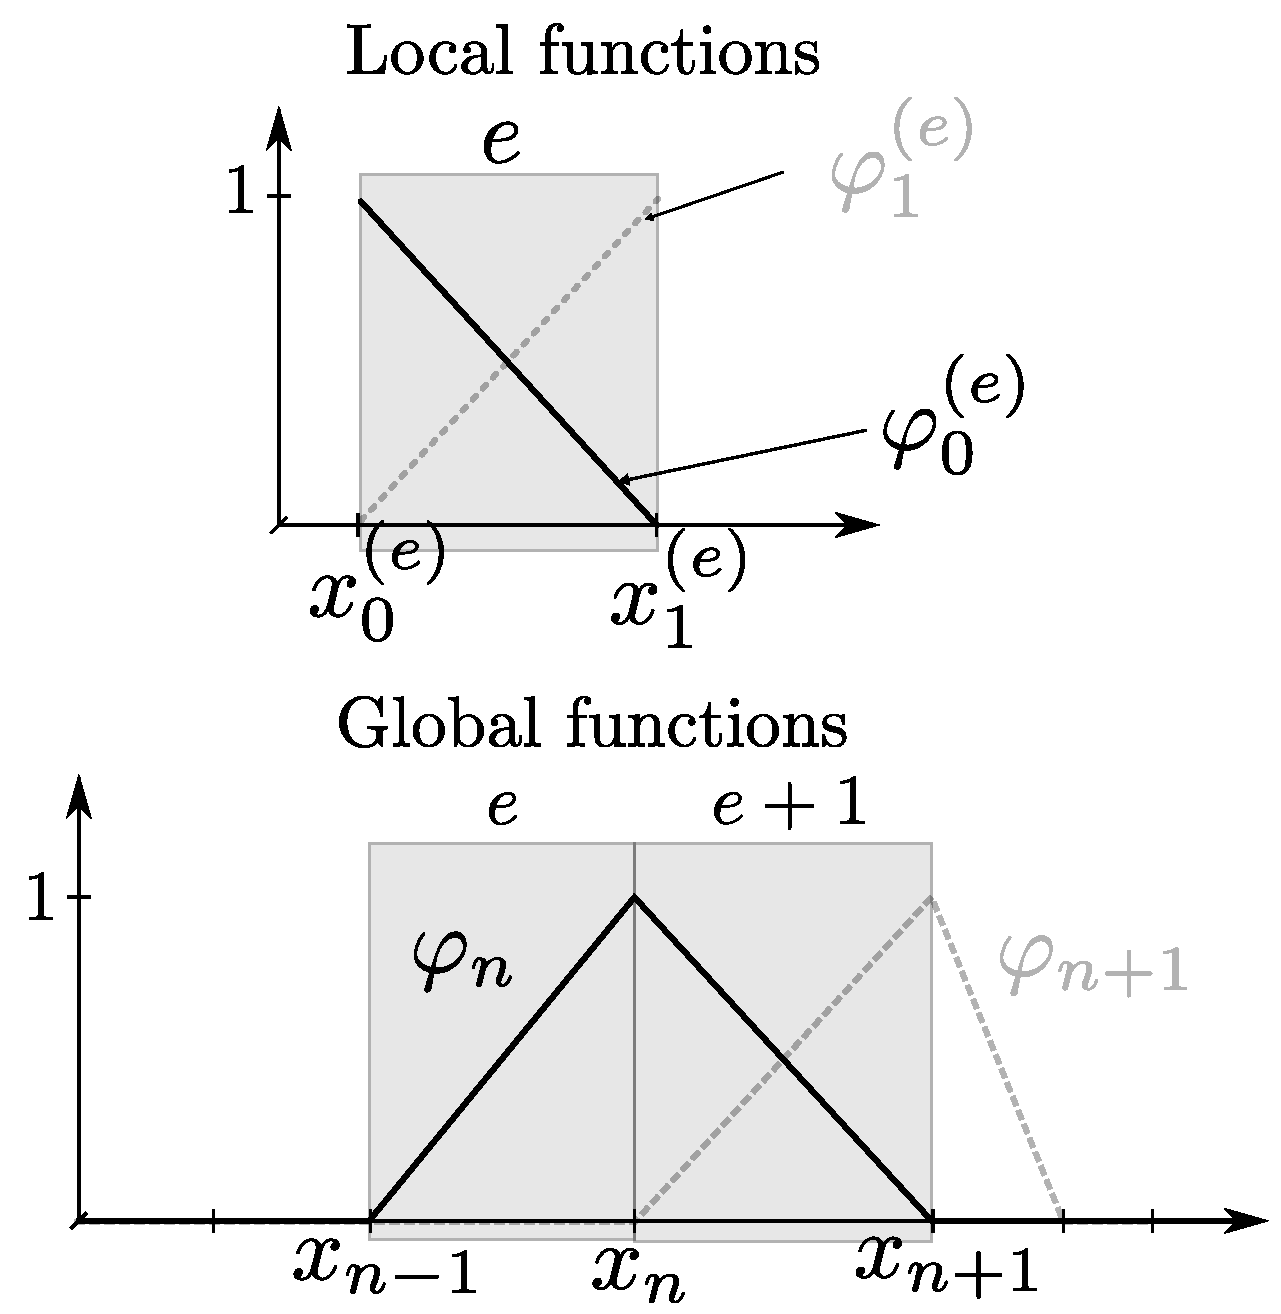
\includegraphics[width=0.8\textwidth]{./images/local_global_functions}
  \caption{The linear Lagrange basis functions and numbering schemes for a one-dimensional
    finite element model.\label{fig:local_global_functions}}
\end{figure}

The global basis functions for are clearly integrable (\ie in $L^2[0,1]$) since
they are just a combination of local basis functions and they satisfy the boundary conditions by definition. So the global basis functions are members of $V_T^h$ and $V_S^h$.

To calculate the matrix $A$ and the vector $\mathbf{b}$ from equation
\eqref{eq:Aij_bj} needed for \eqref{eq:final_galerkin} we first calculate the
local contributions from each element: $A^{(e)}$ and $\mathbf{b}^{(e)}$. Then the
local-to-global mapping tells us which local nodes map to a given global node
and so the global $A$ and $\mathbf{b}$ can be assembled by summing the
appropriate local contributions.

For our one-dimensional Poisson case the calculation of $A^{(e)}$ is quite
simple, substituting the two local basis functions \eqref{eq:32} into
\eqref{eq:Aij_bj} and using $h=x_{1}^{(e)}-x_{0}^{(e)}$ we are left with
\begin{equation*}
  A^{(e)} = \dfrac{1}{h}
  \left[
    \begin{array}{cc}
      1 & -1 \\ -1 & 1
    \end{array}
  \right],
\end{equation*}
where $h$ is the element size, $h = x_{1}^{(e)}-x_{0}^{(e)}$ (note that $h$ can
vary between elements). Similarly for $\mathbf{b}^{{e}}$ we obtain
\begin{equation*}
  \mathbf{b}^{(e)}=\dfrac{1}{h}\left[
    \begin{array}{c}
      -\int_{x_{0}^{(e)}}^{x_{1}^{(e)}}(x-x_{1}^{(e)})\, f(x)\, dx\\
      \int_{x_{0}^{(e)}}^{x_{1}^{(e)}}(x-x_{0}^{(e)})\, f(x)\, dx
    \end{array}\right],
\end{equation*}
which we compute numerically since the entries depend on $f(x)$ which is not yet
decided.


\subsection{Extensions of the Finite Element Method}

\subsubsection{Non-Dirichlet Boundary Conditions}
\label{sub:Non-Dirichlet-Boundary-Conditions}

There are two main types of boundary condition. Dirichlet conditions specify the
\emph{value} at the boundary (as used so far). Neumann conditions specify the
\emph{derivative} at the boundary. These two types can also be mixed together
either as conditions on different parts of the boundary or as a linear
combination of the two (a Robin condition).

Neumann boundary conditions can be added to the finite element method described
above by relaxing the conditions on the shape and test functions at the
boundary. Then the first term in equation~\eqref{eq:29} naturally gives an
additional equation for the Neumann condition on each boundary node.

Combinations of Neumann and Dirichlet conditions on different parts of the boundary can be treated the same way, by restricting the shape and test functions only on the Dirichlet parts.


\subsubsection{Other Equations}
\label{sec:fem-other-equations}

Finite element models are used to solve a wide range of equations including for example applications in fluid/solid mechanics, electrostatics and magnetostatics. There can be various subtleties in the application to different equations but the main difference in the method described so far is the derivation of the weak form. However the same steps of multiplying by a test function and transferring derivatives to the test functions are still used.


\subsubsection{Higher Order Shape/Test Functions}
\label{sec:fem-high-order-shap}

The shape and test functions can also be chosen to be of quadratic, cubic or higher order. This increases the number of nodes required per element (to ensure uniqueness) and increases the difficulty of calculating the integrals. However in some cases the use of higher order polynomials can give a better approximation.


\subsubsection{Higher Dimensions}
\label{sec:fem-higher-dimensions}

The same basic method as given in Sections~\ref{Derivation-of-weighted-residuals} and \ref{sub:Actual-Finite-Elements} can be applied to two and three dimensional problems. Different polynomials for the shape/test functions must be chosen but the basic orthogonality property from equation~\eqref{eq:35} is kept. A larger variety of element shapes are possible -- typically triangular or quadrilateral elements are used in two dimensions and their higher dimension equivalents (tetrahedrons and ``bricks'') are used in three dimensions.


%%% Local Variables:
%%% mode: latex
%%% TeX-master: "./main"
%%% End:


\section{Galerkin's Method for the Landau--Lifshitz--Gilbert Equation}
\label{sec:galerk-meth-llg}

\subsection{Initial Equations}

Our labelling of the domains is shown in Figure~\ref{fig:domain_labels}. We label the region of magnetisable material as $\magd$, it's boundary as $\boundd$ and the external domain as $\extd$.

\begin{figure}[!ht]
  \center
  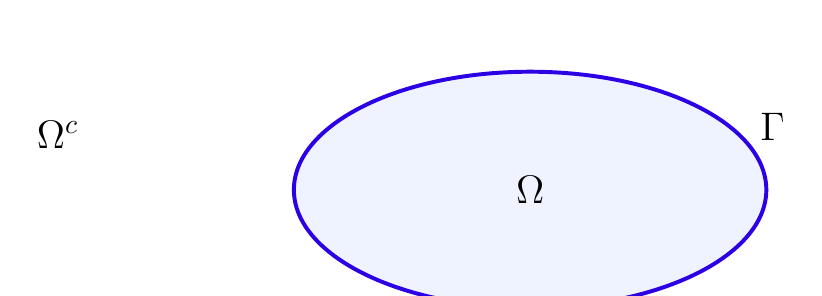
\begin{tikzpicture}
    \draw[line width=0.5mm,fill=paleblue,draw=solidblue] (0,0) ellipse (3cm and 1.5cm);
    \draw (0,0) node {\Large{$\magd$}};
    \draw (2.8,0.8) node[anchor=west] {\Large{$\boundd$}};
    \draw (-6,1) node[anchor=north] {\Large{$\extd$}};
  \end{tikzpicture}
  \caption{The domain labels used: $\magd$ is the magnetic material, $\boundd$ is the boundary and $\extd$ is the (infinite) external region.} \label{fig:domain_labels}
\end{figure}

We start with the Gilbert form of the Landau--Lifshitz--Gilbert equation~\eqref{eq:Gilbert}, the sum of effective fields \eqref{eq:Heff}, the exchange field \eqref{eq:Hex} and the potential method for calculating the magnetostatic field \eqref{eq:Hms} \& \eqref{eq:nnphim}. Note that for simplicity from now on we do not explicitly specify when things are functions of $\xv$ and $t$.

We choose the Gilbert form of the Landau--Lifshitz--Gilbert equation even though it is less immediately intuitive because it greatly reduces the complexity of all derivatations - the Landau--Lifshitz form contains a double cross product and has two terms containing the potentially complicated total field. A side effect of this choice is that explict timestepping schemes cannot be used (since the time dependence is defined implicitly), but as discussed in Section~\ref{sec:model-conclusions} we ill always use implicit timestepping schemes anyway.

The applied field $\Happ$ is known. The crystalline anisotropy field $\Hca$ depends on the type of anisotropy in the magnetic material but it is always just an algebraic function of $\Mv$. For example the most commonly used case of perpendicular anisotropy (caused by hexagonal crystalline structure) gives equation~\eqref{eq:Hca}.

For now we consider the magnetostatic potential only within the magnetic domain, $\magd$, with Neumann or Dirichlet boundary conditions on the boundary, $\boundd$ (see Section~\ref{sec:hybr-finit-elem} for details of the extension to include the external region). We define $\boundd_D$ to represent the region of the boundary domain where a Dirichlet condition is imposed on the magnetostatic potential. Similarly we define $\boundd_\Neu$ to be the region of the boundary where a Neumann condition is imposed. So $ \nabla \phim(\xv) \cdot \nv = g_\Neu(\xv) \; \forall \xv \in \boundd_\Neu$ and $\phim(\xv) = g_D(\xv) \; \forall \xv \in \boundd_D$. Typically we will have either $\boundd_D = \boundd$ or $\boundd_\Neu = \boundd$. We also define the following function spaces for convenience
\begin{align}
  \label{eq:037}
  \Dfs & = \{ v \st v(\xv) \text{ satisfies the b.c. s } \; \forall \xv \in \boundd_D \}, \\
  \Dfs_0 &= \{ v \st v(\xv) = 0 \; \forall \xv \in \boundd_D \}.
\end{align}

\subsection{Normalisation}
\label{sec:normalisation}

For efficient and accurate numerical modelling it is essential to ensure that computed values remain close to unity. As such we actually work in terms of:
\begin{itemize}
\item $\mv = \frac{\Mv}{M_s}$ (non-dimensional)
\item $\hv_{\Box} = \frac{\Hv_\Box}{H_k} = \Hv_\Box \frac{\mu_0 M_s}{2 K_1}$ (non-dimensional), for the applied, exchange and magnetocrystalline anisotropy fields.
\item $t' = \frac{t}{\gymagc H_k}$ (units of .. ??ds)
\end{itemize}
The coefficient of the exchange effective field becomes $\exchc = \frac{2A}{\mu_0 M_s} \cdot \frac{\mu_0 M_s}{2 K_1} = \frac{A}{K_1}$. Both $A$ and $K_1$ have units of energy density\cite{Kronmuller2003} so $\exchc$ is non-dimensional. However this normalisation scheme fails for the case of $K_1 = 0$ (\ie no magnetocrystalline anisotropy), in this case we use $H_A = \frac{2A}{\mu_0 M_s}$ instead.

Now our system of equations is:
\begin{equation}
  \label{eq:llg}
  \dmdt = - \mxh + \dampc \left( \mv \times \dmdt \right),
\end{equation}
\begin{equation}
  \label{eq:heff}
  \hv = \happ + \hca + \hex +  \hms,
\end{equation}

\begin{equation}
  \label{eq:hex}
  \hex = \exchc \nabla^2 \mv,
\end{equation}
\begin{align}
  \hms = - \nabla \phim, \label{eq:hms} \\
  \nabla^2 \phim = \nabla \cdot \mv. \label{eq:phim}
\end{align}





\subsection{Conversion to Weak Form Residuals}

We convert some of the above equations into their residual weak forms as described in Section~\ref{Derivation-of-weighted-residuals}. Each residual equation used increases the complexity of our system of equations, hence we do not rewrite the simple equations for crystalline anisotropy effective field or for the magnetostatic field (in terms of $\phim$) as residuals.


\subsubsection{Magnetostatic Field Residuals}
\label{sec:magn-field-resid}

The equation for the magnetostatic potential becomes \eqref{eq:phim} becomes:
\begin{gather}
  \text{given $\mv \in \sob^1(\magd)$, find $\phim \in \sob^2(\magd) \cap \Dfs$ such that:} \notag \\
  r_{\phim} = \int_\magd (\nabla^2 \phim) v  \d \magd
  - \int_\magd (\nabla \cdot \mv) v \d \magd = 0,
  \quad \forall v \in \sob^0(\magd) \cap \Dfs_0. \label{eqn:phires1}
\end{gather}

The above equation for calculating $\phim$ contains second order derivatives.
We would like to reduce the order of these derivatives as discussed in Section~\ref{Derivation-of-weighted-residuals} to relieve the smoothness requirements on our solution.
We do this by ``transferring'' the derivatives onto the test functions \cite{HowardElmanDavidSilvester2006}.

First we need the following identity\footnote{This can be easily derived by applying the product rule to $\nabla \cdot (v \nabla \phim)$.}
\begin{equation}
  (\nabla^2 \phim) v =
  \nabla \cdot (v \nabla \phim)
  - \nabla \phim \cdot \nabla v.
  \label{eq:20}
\end{equation}
Then integrating over the magnetic domain $\magd$ and applying the divergence theorem gives
\begin{equation}
  \int_\magd (\nabla^2 \phim) v \d \magd =
  \int_{\boundd} v (\nabla \phim \cdot \nv) \d \boundd
  - \int_\magd \nabla \phim \cdot \nabla v \d \magd.
  \label{eqn:identitygauss}
\end{equation}

We now substitute \eqref{eqn:identitygauss} into \eqref{eqn:phires1}, giving
\begin{gather}
   \text{given $\mv \in \sob^1(\magd)$, find $\phim \in \sob^1(\magd) \cap \Dfs$ such that:} \notag \\
  r_{\phim} = \int_{\boundd} v (\nabla \phim \cdot \nv) \d \boundd
  - \int_\magd \nabla v \cdot \nabla \phim \d \magd
  - \int_\magd (\nabla \cdot \mv) v \d \magd = 0
  , \notag \\
  \forall v \in \sob^1(\magd) \cap \Dfs_0. \notag
\end{gather}
This contains only first order derivatives so the solution space for $\phim$ is relaxed to $\sob^1(\magd) \cap \Dfs$. However, all first partial derivatives of the test functions are now required to be integrable, \ie $v \in \sob^1(\magd)$ instead of $v \in \sob^0(\magd)$.

Note that the boundary integral is always zero on the Dirichlet region of the boundary by our definition of the test functions. Hence the boundary integral is only non-zero over $\boundd_{\Neu}$ where we know $(\nabla \phim \cdot \nv) = g_{\Neu}$. Hence we have
\begin{gather}
   \text{given $\mv \in \sob^1(\magd)$, find $\phim \in \sob^1(\magd) \cap \Dfs$ such that:} \notag \\
  r_{\phim} = \int_{\boundd_\Neu} v g_\Neu \d \boundd
  - \int_\magd \nabla v \cdot \nabla \phim \d \magd
  - \int_\magd (\nabla \cdot \mv) v \d \magd = 0
  , \label{res:contphi} \\
  \forall v \in \sob^1(\magd) \cap \Dfs_0. \notag
\end{gather}

% We can also remove the gradient operator from $\mv$ in the second term of \eqref{eqn:phires1} using a similar identity\footnote{Derived by applying the product rule to $\nabla \cdot (\mv v)$ then integrating, multiplying by $4 \pi$ and applying the Divergence theorem.} to \eqref{eqn:identitygauss}
% \begin{equation}
%   - \int_\magd 4 \pi (\nabla \cdot \mv) v \d \magd =
%   4 \pi \int_\magd \mv \cdot (\nabla v) \d \magd
%   - 4 \pi \int_{\boundd} v \mv \cdot \nv \d \boundd.
% \end{equation}

% Substituting this into \eqref{eqn:phires2} leaves us with
% \begin{gather}
%      \text{given $\mv \in \sob^1(\magd)$, find $\phim \in \sob^1(\magd) \cap \Dfs$ such that:} \notag \\
%   r_{\phim} = - \int_\magd \nabla v \cdot \nabla \phim \d \magd
%   + 4 \pi \int_\magd \mv \cdot (\nabla v) \d \magd
%   - 4 \pi \int_{\boundd} v \mv \cdot \nv \d \boundd
%   , \\
%   \forall v \in \sob^1(\magd) \cap \Dfs_0. \notag
% \end{gather}

% \subsubsection{Exchange Field Residuals}
% \label{sec:exch-field-resid}

% The exchange effective field equation~\eqref{eq:hex} becomes:
% \begin{gather}
%    \text{given $\mv \in \sob^2(\magd)$, find $\hex \in \sob^0(\magd)$ such that:} \notag \\
%   \mathbf{r}_{\text{ex}} = \int_\magd \Big( \hex - \exchc \nabla^2 \mv \Big) v \d\magd
%   = 0,
%   \quad \forall v \in \sob^0(\magd).
% \end{gather}

% A similar substitution to \eqref{eqn:identitygauss} can be applied to the residuals for $\hex$. Considering only the $i$th component of $\mathbf{r}_{\text{ex}}$ we have
% \begin{equation}
%   r_{\text{ex},i} = \int_\magd \Big( h_{\text{ex},i} - \exchc \nabla^2 m_i \Big) v \d \magd,
%   \quad \forall v \in \sob^0(\magd).
%   \label{eqn:exresi}
% \end{equation}
% By replacing $\phim$ with $M_i$ in identity \eqref{eqn:identitygauss} and substituting the result into \eqref{eqn:exresi} we obtain
% \begin{gather}
%    \text{given $\mv \in \sob^1(\magd)$, find $\hex \in \sob^0(\magd)$ such that:} \notag
%    \\
%   \mathbf{r}_{\text{ex}} = \int_\magd \hex v \d \magd
%   + \exchc \int_\magd \nabla \mv \cdot \nabla v \d \magd
%   - \exchc \int_{\boundd} v (\nabla \mv \cdot \nv) \d \boundd
%   = 0,
%   \label{res:conthex}
%   \\
%   \forall v \in \sob^1(\magd). \notag
% \end{gather}

\subsubsection{Landau--Lifshitz--Gilbert Equation Residuals}

For the Landau--Lifshitz--Gilbert equation~\eqref{eq:llg} we have a set of three residuals per test function. For now we sidestep the details of time discretisation by assuming $\dmdt$ to be just another function of $\xv$ that we can solve for.
\begin{gather}
  \text{given $\hv \in \sob^0(\magd)$ and $\mv \in \sob^1(\magd)$ find $\dmdt \in \sob^1(\magd)$ such that:} \notag
  \\
  \mathbf{r}_{\text{llg}} = \int_\magd \Big( \dmdt
  + (\mv \times \hca) + (\mv \times \happ) \\
  - (\mv \times \nabla \phi) + \exchc(\mv \times \nabla^2 \mv)
  - \dampc \left( \mv \times \dmdt \right)
  \Big)  v \d\magd
  = 0, \label{res:contllg}
  \\
  \forall v \in \sob^0(\magd). \notag
\end{gather}

We again wish to reduce the order of the derivatives, this time on $\mv$ in
\begin{equation}
 I = \int_\magd (\mv \times \nabla^2 \mv) v \d\magd.
 \label{eq:46}
\end{equation}
It can be shown that this is equivalent to
\begin{equation}
  \label{eq:49}
  I = - \int_\magd  \mv \times \threevec{\nabla v \cdot \nabla m_1}{\nabla v \cdot \nabla m_2}{\nabla v \cdot \nabla m_2} \d\magd + \int_\boundd (\mv \times \pd{\mv}{\nv}) v \d\boundd,
\end{equation}
using similar techniques to those in Section~\ref{sec:magn-field-resid}. %??ds derivation in appendix? I've written it down in notebook begining 22/9/11 near the end.

??ds can we assume $(\mv \times \pd{\mv}{\nv}) = 0$? Others do... will do for now

\subsection{Spatial Discretisation}
\label{sec:spat-discr-resi}

The next step is to discretise the residuals in space. As in Section~\ref{Derivation-of-weighted-residuals} and \ref{sub:Actual-Finite-Elements} we replace continuous variables and functions by a basis representation using a finite space of shape functions. We also replace the infinite spaces of test functions used so far by finite dimensional approximations.

We choose the solution space to be the same as the test function space (except for boundary conditions), this choice makes our method a Galerkin method. We also choose the shape/test functions to be the same for all residuals/unknowns. So the infinite dimensional space used for all shape and test functions is $\sob^1(\magd)$ with appropriate boundary conditions.

We then replace the space $\sob^1(\magd)$ by the $N$-dimensional approximation $\ts \subset \sob^1(\magd)$. In this approximation the unknowns $\mv$, $\hex$ and $\phim$ can be represented anywhere in the domain as a sum over the nodal values multiplied by the shape function, $\sk \in \ts$, for that node:
\begin{gather} % \sk = shapefn_k
  \mv = \sum_{k = 0}^{N} \sk \, \mv_k, \quad
  \hex = \sum_{k = 0}^{N} \sk \, \hex_{,k}, \quad
  \phim = \sum_{k = 0}^{N} \sk \, \phim_{,k}.
  \label{eq:unknowns-basis}
\end{gather}
Similarly the test functions can be approximated by a sum over the test basis functions, $\tn \in \ts$, as
\begin{equation}
  \label{eq:47}
  v = \sum_{\ndi = 0}^{N} \tn \, a_\ndi.
\end{equation}
Note that in our method $\sbf_k \equiv \tbf_k$, but we continue to write the two functions differently for generality. Also the basis functions for the space of test functions are often simply refered to as the test functions since they are used equivalently.

So substituting the basis representations, \eqref{eq:unknowns-basis} and \eqref{eq:47} into the residuals we obtain a spatially discretised version of the problem. Out of necessity we have used Einstein summation notation below - two terms with a matching index multiplied together indicates a sum over all values of that index.
\begin{gather}
  \label{res:tintro}
  \text{Given $\happ(\xv,t)$ and $\hca(\xv,t)$, $\forall k$, $\forall \ndi$ find} \notag \\
  \phim_{,k} \in \ts \cap \Dfs, \quad
  \mv_{k} \in \ts \text{ and }
  \pd{\mv_k(t)}{t} \in \ts \notag
\end{gather}
such that
\begin{align}
  r_{\phim, \ndi} =
  & - \int_{\magd} (\nabla \tn \cdot \nabla \sk) \phim_{,k} \d \magd \notag
  - \int_{\magd} (\nabla \cdot (\mv_{k} \sk) ) \tn \d \magd \\
  & + \int_{\boundd_{\Neu}} \tn g_\Neu \d \boundd = 0,
  \label{res:tphi}
\end{align}
% \begin{align}
%   \mathbf{r}_{\text{ex},\ndi} =  & \int_{\magd} \tn \sk \hex_{,k} \d \magd
%   \quad + \exchc \int_{\magd} (\nabla \sk \cdot \nabla \tn) \mv_{k} \d \magd \notag \\
%   &- \exchc \int_{\boundd} \tn (\nabla \sk \cdot \nv) \mv_{k} \d \boundd  = 0,
% \label{res:thex}
% \end{align}
\begin{align}
 \mathbf{r}_{\text{llg},\ndi} &=
 \mathbf{r}_{\text{llgexch},\ndi} +  \int_{\magd} \tn \sk \pd{\mv_k}{t} \d \magd \notag \\ %??ds no
  &- \int_{\magd} (\mv_k \sk) \times ( \phim_{,k} \nabla \sk) \tn \d \magd \notag \\
  &+ \int_{\magd} (\mv_k \sk) \times ( \hca(\mv_k\sk) + \happ) \tn \d \magd \notag \\
 % &+ \dampc \int_{\magd}  (\mv_k\sk) \times \Big( (\mv_k \sk) \times (\hv_k \sk) \Big)  \tn \d \magd = 0,
  &- \dampc \int_{\magd}  (\mv_k\sk) \times \left( \sk \pd{\mv_k}{t} \right) \tn \d \magd = 0,
  \label{res:tllg}
 % \text{where } \hv_k &= \hex_{,k} - \nabla \phim_{,k} + \happ + \hca. \notag
\end{align}

\begin{equation}
  \mathbf{r}_{\text{llgexch},\ndi} = - \int_\magd (\mv_k \sk) \times
  \threevec{\nabla \tn \cdot (m_{1,k} \nabla \sk)}{\nabla \tn \cdot (m_{2,k} \nabla \sk)}{\nabla \tn \cdot (m_{3,k} \nabla \sk)} \d\magd
\end{equation}

Note that we could move the discretised values of the unknowns outside of the integrals because they are constant in space. However we prefer to evaluate values at points within the elements where possible (by integrating using Gaussian quadrature) since some quantities are discontinous at the nodes.\footnote{For example if the basis functions are linear then derivatives are discontinous at the nodes.}

Also note that we have $7N$ equations in $7N$ unknowns and each of the integrals in the equations can be evaluated only in terms of the shape/test functions, their derivatives, the outward unit normal vector and the Neumann boundary condition. Hence we have a system of algebraic equations which we can solve.

As described in Section~\ref{sub:Actual-Finite-Elements} we can convert this ``global'' representation into a number of ``local'' representations -- one on each element. We first split the domain into $N_e$ elements. We then define the basis functions such that they are only non-zero on elements in which they are contained (\ie we are using a finite element method). Then the global residuals can be split into the local contributions each element which are easy to calculate since they only depend on nodes within the element.\footnote{Unfortunately this property will be lost to some extent when we introduce the hybrid FEM/BEM in Section~\ref{sec:hybr-finit-elem}.}

Let $\magd_\eli$ represent the volume of element $e$, let $\boundd_\eli$ represent any part of the boundary of the element which is on $\boundd$ (nothing for most elements). Then the contribution of element $\eli$ to the residuals at node $\ndi$ is exactly as given in equations~\eqref{res:tintro}-\eqref{res:tllg} except that the integrations are performed over $\magd_\eli$ and $\boundd_\eli$ rather than $\magd$ and $\boundd$. Also note that the sums only need to consider values of $k$ such that node $k$ is in element $\eli$ and that residual contributions only need to be calculated for nodes $\ndi$ such that node $\ndi$ is in element $\eli$.

% \begin{align}
%   r_{\phim, \ndi, \eli} = \sum_{k} \Bigg[ &
%   - \phim_{,k} \int_{\magd_\eli} \nabla \tn \cdot \nabla \sk \d \magd \notag
%   - \mv_{k} \int_{\magd_\eli} (\nabla \cdot \sk ) \tn \d \magd \Bigg] \\
%   &+ \int_{\boundd_{\Neu,\eli}} \tn g_\Neu \d \boundd,
%      \label{res:tphi}
%      \\
%   \mathbf{r}_{\text{ex}, \ndi, \eli} = \sum_k \Bigg[ & \hex_{,k} \int_{\magd_\eli} \sk \tn \d \magd
%   \quad + \exchc \mv_{k} \int_{\magd_\eli} \nabla \sk \cdot \nabla \tn \d \magd \notag \\
%    &- \exchc \mv_{k} \int_{\boundd_\eli} \tn (\nabla \sk \cdot \nv) \d \boundd \Bigg],
%    \label{res:thex}
%    \\
%   \mathbf{r}_{\text{llg}, \ndi, \eli} = \sum_k \Bigg[ &
%   \pd{\mv_k}{t} \int_{\magd_\eli} \sk \tn \d \magd
%   \quad +(\mv_k \times \hv_k) \int_{\magd_\eli} \sk^2 \tn \d \magd \notag \\
%   &+ \dampc \Big( \mv_k \times (\mv_k \times \hv_k) \Big) \int_{\magd_\eli} \sk^3 \tn \d \magd \Bigg] , \label{res:tllg}
%   \\
%   \text{where } \hv_k &= \hex_{,k} - \nabla \phim_{,k} + \happ + \hca.
% \end{align}

\subsection{Time Discretisation}
\label{sec:time-discretisation-resi}

To deal with the time derivative in equation~\eqref{res:tllg} we must apply a time discretisation scheme. As discussed in Section~\ref{sec:model-conclusions} we aim to use the mid-point method in our model, however so far the backwards difference method has been used for implementation convenience.

Let $h$ be the time-step, let $\mv_k^\tl$ denote the value of $\mv_k$ at the $\tl$-th time-step, and consider only the value of $\mv_k$ at a single node. Then the mid-point method is defined by d'Aquino\cite{DAquino2005} as
\begin{equation}
  \label{eq:mid-point-scheme}
  \dmdt \left( \frac{\mv_k^{\tl+1} + \mv_k^\tl}{2} \right) = \frac{\mv_k^{\tl+1} - \mv_k^l}{ h}.
\end{equation}
So by substituting equation~\eqref{eq:mid-point-scheme} into equation~\eqref{res:tllg} with $\mv_k = \frac{\mv_k^{\tl+1} + \mv^\tl_k}{2}$ we obtain a fully discretised system of equations for $\mv_k^{\tl+1}$ in terms of $\mv_k^\tl$.

The second order backwards difference method is defined as\cite{Atkinson2009}
\begin{equation}
  \label{eq:bdf2-scheme}
  \dmdt(\mv_k^{\tl+1}) = \frac{3 \mv_k^{\tl+1} - 4 \mv_k^{\tl} + \mv_k^{\tl-1}}{2h},
\end{equation}
which can similarly be substituted into equation~\eqref{res:tllg} with $\mv_k = \mv_k^{\tl+1}$ to obtain a fully discretised system of equations for $\mv_k^{\tl+1}$ in terms of $\mv_k^\tl$ and $\mv_k^{\tl-1}$.

%%% Local Variables:
%%% mode: latex
%%% TeX-master: "main"
%%% End:



\section{Hybrid Finite/Boundary Element Method}
\label{sec:hybr-finit-elem}
The hybrid finite/boundary element method works similarly to the normal finite element method except that one or more sub-regions are mapped onto their boundary \cite{Rammohan2002}.
The main advantage of this is that we reduce the dimensionality of these sub-regions one since we only have to solve equations on the boundary instead of the entire space.
In our case this is likely to give an advantage over a pure finite element method since we no longer need to mesh a long way outside the magnetic domain to accurately account for the effect of the external region. Also other methods for dealing with infinite domains can often give additional errors due to the truncation of the external domain.\cite{Bottauscio2008}

On the downside this mapping typically results in a dense matrix after discretisation, to which we cannot apply sparse matrix techniques.
Also the integrals that need to be computed may involve singularities, which introduce additional complications and may reduce accuracy or increase computation time.

Note that the derivation for this hybrid method comes from potential theory, rather than the boundary integral formulation usually used to construct the standard boundary element method.

\subsection{Background of the Method}
\label{sec:basic-method}
We want to use the boundary element method in the calculation of the magnetostatic scalar potential $\phim$, ($\hms = - \nabla \phim$), in the infinite region outside of a magnetic body.
Using the boundary element method directly, however, would require the solution of dense matrix equations for the entire problem.

We can circumvent this problem by splitting the potential into two parts $\phim = \phi_1 + \phi_2$ in such a way that $\phi_1$ can be calculated the magnetic region(s) using only the finite element method.
We then have some conditions on $\phi_2$ that must be satisfied to give the correct total potential in $\magd$ and on $\boundd$, but, in order to solve for $\phi_2$ in the magnetic domain, we still need to find the boundary conditions (on the edge of the magnetic domain).
So we choose a charge distribution on the boundary that satisfies all the conditions on $\phi_1$ and $\phi_2$.
We can then solve for $\phi_2$ on the boundary using similar techniques to those used in the boundary element method.
Finally we apply the finite element method to find $\phi_2$ inside the magnetic region $\magd$.

By the uniqueness of solution for Poisson's equation with Dirichlet and/or Neumann boundary conditions we know that the field $ \hms = \nabla \phim$  constructed by the above steps is \emph{the} magnetostatic field.\footnote{To see this take the difference of two solutions of Poisson's equation: $\phi = \psi_1 - \psi_2$. Then using identity \eqref{eq:20}, the linearity of Poisson's equation and the divergence theorem we obtain $\int_S \phi \nabla \phi \cdot d \mathbf{S} = \int_V (\nabla \phi)^2 dV$. Applying Dirichlet, Neumann or mixed boundary conditions shows that the boundary integral is zero and hence $\nabla \phi = 0$.}

\subsection{Problem Description}
\label{sec:problem-description}
Let $\phi^\inte$ be the value of $\phi$ (with subscripts as appropriate) close to the boundary $\boundd$ and just inside the magnetic domain  and $\phi^\exte$ the value of $\phi$ just outside the magnetic domain\footnote{More precisely $\phi^\inte(\xv) = \lim_{\xv \rightarrow \boundd} \phi(\xv)$ from inside the magnetic domain, $\phi^\exte(\xv) = \lim_{\xv \rightarrow \boundd} \phi(\xv)$ from outside the magnetic domain.} (see Figure~\ref{fig:BEM-geometry}).

\pagebreak % Be careful with this...

We have the following \emph{physical} conditions\footnote{Equations~\eqref{eq:2}-\eqref{eqn:phibound} come from the definition of $\phi_m$, requirement for finite total energy, $\Bv^\text{int} \cdot \nv = \Bv^\text{ext} \cdot \nv$ and ??ds respectively.} on the total magnetostatic potential $\phim$:
\begin{equation}
  \nabla^2 \phim(\xv) = \nabla \cdot \mv(\xv) \qquad \forall \xv \in \magd \cup \extd,
  \label{eq:2}
\end{equation}
\begin{equation}
  \phim(\xv) \rightarrow 0 \qquad \text{ as } |\xv| \rightarrow \infty,
\end{equation}
\begin{equation}
  \pd{\phim^\inte(\xv)}{\nv} - \pd{\phim^\exte(\xv)}{\nv} = \mv \cdot \nv \qquad \xv \in \boundd,
  \label{eqn:dphibound}
\end{equation}
\begin{equation}
  \phim^\inte(\xv) - \phim^\exte(\xv)  = 0 \qquad \xv \in \boundd.
  \label{eqn:phibound}
\end{equation}
Note that equations~\eqref{eqn:dphibound} and \eqref{eqn:phibound} imply continuity but not smoothness of the magnetic potential $\phim$ across $\boundd$. This is due to surface magnetic charges.

We choose $\phi_1$ to satisfy:
\begin{equation}
  \phim(\xv) = \phi_1(\xv) + \phi_2(\xv) \qquad \forall \xv \in \fulld,
  \label{eq:21}
\end{equation}
\begin{equation}
  \nabla^2 \phi_1(\xv) = \nabla \cdot \mv(\xv) \qquad \xv \in \magd,
  \label{eq:1}
\end{equation}
\begin{equation}
  \pd{\phi^\inte_1(\xv)}{\nv} = \mv \cdot \nv \qquad \xv \in \boundd,
  \label{eqn:dphionebound}
\end{equation}
\begin{equation}
  \phi_1(\xv) = 0 \qquad \xv \in \extd.
  \label{eqn:phioneoutside}
\end{equation}
Note that equations~\eqref{eq:1} and \eqref{eqn:dphionebound} give a self contained Poisson Neumann problem for $\phi_1 \in \magd \cup \boundd$.

The equations~\eqref{eq:2} to \eqref{eqn:phibound} for $\phim$ combined with equations~\eqref{eq:21} to \eqref{eqn:phioneoutside} for $\phi_1$ give a number of conditions on $\phi_2$ must satisfy. Since the Laplacian operator is linear, \ie $\nabla^2 \phim = \nabla^2 \phi_1 + \nabla^2 \phi_2$, from \eqref{eq:2} and \eqref{eq:1} it follows that
\begin{equation}
  \label{eq:8}
  \nabla^2 \phi_2(\xv) = 0 \qquad \forall \xv \in \fulld.
\end{equation}

Equation~\eqref{eqn:phioneoutside} implies that $\pd{\phi^\exte_1(\xv)}{\nv} = 0$. Combining this with equations (\ref{eqn:dphionebound}) and (\ref{eqn:dphibound}) gives
\begin{equation}
  \label{eq:5}
  \pd{\phi^\inte_2(\xv)}{\nv} - \pd{\phi^\exte_2(\xv)}{\nv} = 0.
\end{equation}

Finally from equations (\ref{eqn:phibound}), \eqref{eq:21} and (\ref{eqn:phioneoutside}) we have
\begin{equation*}
  \phi^\inte_1 - \phi^\exte_1 + \phi^\inte_2 - \phi^\exte_2 = 0,
\end{equation*}
\begin{equation}
  \phi^\inte_2 - \phi^\exte_2 = - \phi^\inte_1.
\label{eq:4}
\end{equation}

\begin{figure}
  \center
  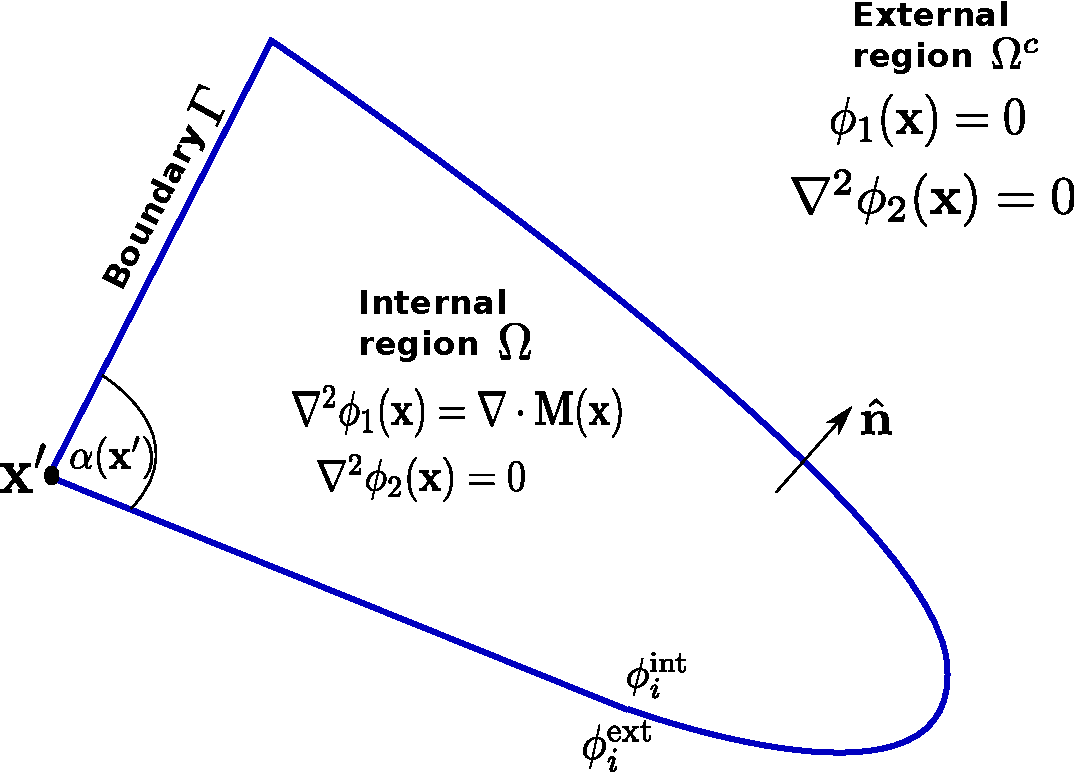
\includegraphics[width=0.75\textwidth]{./images/BEM-geometry}
  % \begin{tikzpicture}

  %   % Main nodes and some labels
  %   \node[label=below:$\xv'$] (a) at (-2,-2) {};
  %   \node (b) at (-2,2) {};
  %   \node[label=right:\Large{$\boundd$}] (c) at (5,0) {};

  %   % Draw main shape of magnetic domain
  %   \draw [line width=0.5mm,draw=solidblue,fill=paleblue] (a.north) to [bend right=71] (c) to (b.south);
  %   \draw [line width=0.5mm,draw=solidblue] (a) to (b);
  %   \draw (a.north) circle(1mm) [fill=black] {};

  %   % More labels
  %   \node (center) at (1,0) {\Large{Magnetic domain $\magd$}};
  %   \node(external) at (8,3) {\Large{External region $\extd$}};
  % \end{tikzpicture}

  \caption{A 2D representation of the geometry showing the labels used in this section. The point $\xv'$ is a singular point of the boundary $\boundd$, the angle $\alpha(\xv')$ is as shown.}
  \label{fig:BEM-geometry}
\end{figure}

\subsection{Double Layer Potentials}
\label{sec:double-layer-potent}
A double layer potential can be thought of as the potential due to a layer of dipoles of magnitude $\mu(\xv)$ in direction $\nv$ over the surface $S$.\cite{Sternberg1946} We will demonstrate that we can use a double layer potential to calculate $\phi^\inte_2$ in terms of $\phi^\inte_1$.

The double layer potential at a point $\xv \in \real^d$ is defined as \cite{eom_double_layer_potential}
\begin{equation}
  \label{eq:3}
  \phi(\xv) = \int_{S} \mu(\yv) \pd{\Green}{\nv} \d \yv,
\end{equation}
where $G$ is the Green's function for a Laplacian operator.
For $d=2$
\[ \Green = \dfrac{-1}{2\pi}\ln(|\xv - \yv|), \]
and for $d=3$
\begin{equation} \Green = \dfrac{-1}{4 \pi} \dfrac{1}{|\xv - \yv|}.
  \label{eqn:greenslaplacian3d}
\end{equation}


We have the following results from potential theory:\cite{Sternberg1946}
\begin{enumerate}
\item The double layer potential satisfies Laplace's equation $\nabla^2 \phi = 0$ (in other words the double layer potential is harmonic).% pages ?

\item The double layer potential undergoes a jump of $\mu(\xv)$ moving in the direction $\nv$ across a smooth surface $S$, \ie
  \begin{equation}
    \label{eq:15}
    \phi^\inte(\xv) - \phi^\exte(\xv) = \mu(\xv).
  \end{equation}
% pages 136-140

\item For $\xv \in S$ the following relationship holds
  \begin{equation}
    \phi^\inte(\xv) = (1 - \frac{\alpha(\xv)}{\alpha_{\text{max}}}) \mu(\xv) + \phi(\xv),
    \label{eq:22}
  \end{equation}
  where $\alpha(\xv)$ is the angle (or solid angle) in two (or three) dimensions subtended by the domain at $\xv$ and
\begin{equation*}
  \alpha_{\text{max}} =
  \begin{cases}
    2 \pi & \text{if } d=2 \\
    4 \pi & \text{if } d=3.
  \end{cases}\label{eq:16}
\end{equation*}
Note that $\alpha(\xv)$ is the angle at the exact point $\xv$, when the surface at $\xv$ is a Lyapunov surface (\ie not a sharp corner) $\frac{\alpha(\xv)}{\alpha_{\text{max}}}$ reduces to a factor of $1/2$. We write $\gamma(\xv) = \frac{\alpha(\xv)}{\alpha_{\text{max}}}$ for simplicity.
 % pages 137-139, page 155 for 2d

\item If $\mu$ is continuous and has continuous first and second derivatives along the boundary (\ie $\mu(\xv) \in C^2[S]$) then the limits $\pd{\phi^\inte(\xv)}{\nv}$ and $\pd{\phi^\exte(\xv)}{\nv}$ exist and are equal. % pages 145-153.

\end{enumerate}

Some notes on the derivation of the above results in Sternberg 1946\cite{Sternberg1946}:
\begin{itemize}
\item Some derivations of the results above rely on the surface being a ``Lyapunov surface'' which imposes a number of smoothness conditions, in particular excluding surfaces with corners.
The proofs given in Sternberg allow a finite number of sharp corners, \ie a polygonal domain.
\item Our potentials are a factor of $\frac{-1}{4 \pi}$ different from those in the reference. Also our $\phi^\inte$ and $\phi^\exte$ definitions correspond respectively to $\phi^-$ and $\phi^+$ in the book.
\end{itemize}

\subsection{Application to Magnetostatic Calculations}
From Section~\ref{sec:double-layer-potent} we can see that conditions \eqref{eq:8}, \eqref{eq:5} and \eqref{eq:4} on $\phi_2$ are satisfied by a double layer potential with magnitude
\begin{equation}
  \label{eq:24}
  \mu(\xv) = - \phi^\inte_1(\xv).
\end{equation}

By the uniqueness of solution for Poisson's equation this gives us, up to an additive constant, the only solution for $\phi_2(\xv)$ in the external region.
This is good enough for a potential since it is only used in $\hms(\xv) = - \nabla \phim(\xv)$ so addition of a constant has no effect.

From equations~\eqref{eq:3}, \eqref{eq:22} and \eqref{eq:24} we have:
\begin{equation}
  \label{eq:6}
  \phi^\inte_2(\xv) =  \big(\gamma(\xv) - 1 \big) \phi^\inte_1(\xv)
  - \int_{\boundd} \phi^\inte_1(\yv) \pd{\Green}{\nv} \d \yv.
\end{equation}
After substituting in our definition for the three dimensional Green's function \eqref{eqn:greenslaplacian3d} we obtain the same equation as given by Koehler \cite{Koehler1997}.
Similar equations are solved when using the standard boundary element method, hence the name.

Also note that $\phim = \phi_1 + \phi_2$ everywhere and so
\begin{align}
  \label{eq:18}
  \phim^\inte(\xv) &= \bm \big[ \phi^\inte_1(\xv) \big] \\
  &= \gamma(\xv) \phi^\inte_1(\xv)
  - \int_{\boundd} \phi^\inte_1(\yv) \pd{\Green}{\nv} \d \yv. \notag
\end{align}

Either equation~\eqref{eq:6} or \eqref{eq:18} can be used to give boundary conditions for $\phi_2 \in \magd$ or $\phim \in \magd$ respectively. We will proceed using equation~\eqref{eq:18} for simplicity since it eliminates $\phi_2$ from later calculations.

 Hence, given the solution for $\phi_1 \in \boundd$ (from solving \eqref{eq:1} and \eqref{eqn:dphionebound}) we have a complete Dirichlet Poisson problem for $\phim \in \magd \cup \boundd$:
\begin{align}
  \label{eq:phim-bem}
  \nabla^2 \phim(\xv) = \nabla \cdot \mv(\xv) \quad \xv \in \magd, \\
  \phim(\xv) = \bm \big[ \phi_1(\xv) \big] \quad \xv \in \boundd.
\end{align}

\subsection{Discretisation}
\label{sec:discretisation}

Given the operator $\bm$ the discretisation of equations~\eqref{eq:phim-bem}, \eqref{eq:1} and \eqref{eqn:dphionebound} is simple. We use standard finite elements as described in Section~\ref{sub:Actual-Finite-Elements}. We approximate $\phi^\inte_1$ and $\phi^\inte_2$ as the sum of a finite set of basis functions where each basis function corresponds a single node on the boundary $\boundd$. We will use test and shape functions identical except for boundary conditions to those used in Section~\ref{sec:spat-discr-resi}. So for $\phim$ the test functions are $\tbf_{\text{m}} \in \ts \cap \Dfs$, $\;\Dfs = \{ \tbf \st \tbf(\xv) \text{ satisfies the b.c. s } \; \forall \xv \in \boundd_D \}$. For $\phi_1$ they are $\tbf_1 \in \ts$ since we only have Neumann boundary conditions.

Hence the calculation of $\phi_1$ proceeds exactly as described in Section~\ref{sec:spat-discr-resi} with pure Neumann boundary conditions ($\boundd_\Neu = \boundd$ and $g_\Neu = \mv \cdot \nv$). Once we have the boundary conditions the calculation of $\phim$ proceeds similarly but with pure Dirichlet conditions ($\boundd_D = \boundd$). Therefore all that remains to be discretised is the operator $\bm$. We let
\begin{equation}
  \phim^\inte = \sum_\ibasis \phim_{,\ibasis}^\inte \tbf_{\text{m},\ibasis}(\xv),
  \qquad
  \phi^\inte_1 = \sum_\ibasisb \phi^\inte_{1,\ibasisb} \tbf_{1,\ibasisb}(\xv),
  \label{eq:25}
\end{equation}
where $\tbf_\ibasis(\xv_\ibasisb) = \delta_{\ibasis \ibasisb}$ on the boundary nodes and is linearly interpolated from $\tbf_\ibasis = 1$ at $\xv_\ibasis$ to $\tbf_\ibasis = 0$ at neighbouring nodes.

Substituting equations~\eqref{eq:25} into \eqref{eq:18} we have
\begin{equation*}
  \sum_\ibasis \phim_{,\ibasis}^\inte \tbf_{\text{m},\ibasis}(\xv) =
  - \int_{\boundd} \sum_\ibasisb \phi^\inte_{1,\ibasisb} \tbf_{1,\ibasisb}(\yv)
  \pd{\Green}{\nv} \d \yv
  \quad + \gamma(\xv) \sum_\ibasisb \phi^\inte_{1,\ibasisb} \tbf_{1,\ibasisb}(\xv).
\end{equation*}

To get the value of $\phim^\inte$ at node $\ibasisc$ we choose $\xv = \xv_\ibasisc$. Then using the property $\tbf_\ibasis(\xv_\ibasisc) = \delta_{\ibasis \ibasisc}$ and replacing $\ibasisc$ by $\ibasis$ we have
\begin{equation}
  \phim_{,\ibasis}^\inte =
  - \int_{\boundd_\ibasisb} \sum_\ibasisb \phi^\inte_{1,\ibasisb} \tbf_{1,\ibasisb}(\yv)
  \pd{\Green[\ibasis]}{\nv} \d \yv
  \quad + \gamma(\xv_\ibasis) \phi^\inte_{1,\ibasis},
  \label{eq:colocation}
\end{equation}
where ${\boundd_\ibasisb}$ is the region where $\tbf_{1,\ibasisb} \neq 0$, \ie the elements which contain node $\ibasisb$.

Finally, since the integrands are continuous functions ??ds citation needed, we can move the sum outside the integral leaving
\begin{equation}
  \phim_{,\ibasis}^\inte =
  - \sum_\ibasisb \phi^\inte_{1,\ibasisb} \Big[ \int_{\boundd_\ibasisb} \tbf_{1,\ibasisb}(\yv)
  \pd{\Green[\ibasis]}{\nv} \d \yv \Big]
  \quad + \gamma(\xv_\ibasis) \phi^\inte_{1,\ibasis}.
\label{eq:27}
\end{equation}
Notice that the expression inside the square brackets is independent of all the potentials: it depends only on the geometry and so can be pre-calculated and stored in many cases.

So equation~\eqref{eq:27} gives $\phim^\inte$ at a boundary node in terms of a sum of geometric factors multiplied by $\phi^\inte_1$ at each boundary node.
In other words, this is a dense matrix multiplication by a pre-computed matrix giving $\phim^\inte$ at all the boundary nodes in terms of $\phi^\inte_1$ at all boundary nodes:
\begin{equation}
  \label{eq:10}
  \phim_{,\ibasis}^\inte = \bm_{\ibasis,\ibasisb} \cdot \phi_{1,\ibasisb}^\inte,
\end{equation}
where
\begin{equation}
  \label{eq:17}
  \bm_{\ibasis\ibasisb} = - \int_{\boundd_\ibasisb} \tbf_{1,\ibasisb}(\yv) \pd{\Green[\ibasis]}{\nv} \d \yv
  \quad + \gamma(\xv_\ibasis)\delta_{\ibasis\ibasisb}.
\end{equation}


% ??ds wrong place for this discussion and not sure if integral is really singular or not due to the n.r term...
%Note that although this integral appears at first glance to be singular when the node $\xv_\ibasis$ is within $\boundd_\ibasisb$ (the line segment or section of surface being integrated over)
%A benefit of this is that the matrix is always well conditioned because the largest terms are near the singularity and hence near the diagonal elements $\ibasisb = \ibasis$.
%However the singularity can cause difficulties in the evaluation of the affected integrals.
%Methods to overcome these difficulties are discussed in the next section.

We now convert the normal derivative of the Green's function into a more tangible form.
In 3D
\begin{equation}
  \label{eq:11}
  \pd{\Green}{\nv} = \frac{-1}{4 \pi} \pd{}{\nv} \Gthreed = \frac{-1}{4 \pi} \nv \cdot \nabla \Big( \Gthreed \Big).
\end{equation}
Converting to spherical coordinates with the origin at $\xv_\ibasis$ ($r = |\yv - \xv_\ibasis|$, $\ruv = \frac{\yv - \xv_\ibasis}{r}$) we have
\begin{equation}
  \label{eq:12}
  \pd{G(r)}{\nv} = \frac{-1}{4 \pi} \nv \cdot \ruv \pd{}{r} \Big( \frac{1}{r} \Big)
  = \frac{+1}{4 \pi}  \frac{\nv \cdot \ruv}{r^2}
  = \frac{\nv \cdot \rv}{4 \pi |\rv|^3}
  ,\footnote{In spherical polar coordinates $\nabla = \ruv \pd{}{r} +  \phiv \frac{1}{r} \pd{}{\phi} + \thetav \frac{1}{r \sin \theta} \pd{}{\theta}$. Obviously $\frac{1}{r}$ has no angular dependence so only the derivative with respect to $r$ is non-zero.}
\end{equation}
\begin{equation}
  \label{eq:13}
  \pd{\Green}{\nv} = \frac{\nv \cdot \ruv}{4 \pi |\yv - \xv_\ibasis| ^2} .
\end{equation}
Similarly in 2D we find
\begin{equation}
  \label{eq:14}
  \pd{\Green}{\nv} = \frac{-1}{2 \pi} \pd{}{\nv} (\Gtwod) = \frac{\nv \cdot \ruv}{2 \pi |\yv - \xv_\ibasis|}.
\end{equation}

So the discretised boundary element matrix in $d=2,3$ dimensions is
\begin{equation}
  \label{eq:19}
  \bm_{\ibasis\ibasisb} =\frac{-1}{2^{(d-1)} \pi} \int_{\boundd_\ibasisb} \tbf_{1,\ibasisb}(\yv) \frac{\nv(\yv) \cdot \ruv_{\xv_{\ibasis} \rightarrow \yv}}{|\yv - \xv_\ibasis| ^{d-1}} \d \yv
   \quad + \gamma(\xv_\ibasis)\delta_{\ibasisb\ibasis},
\end{equation}
where the subscript on $\ruv_{\xv_{\ibasis} \rightarrow \yv}$ is to remind us that the unit vector goes from $\xv_j$ to $\yv$.  We denote the integral in this equation by $I_\bm$.

\subsection{Discussion}

\subsubsection{Discretisation Approaches: Co-location vs Galerkin}

Note that in the above we have used a co-location approach to discretisation
??ds where?

??ds difference

??ds implications, why can't we use Galerkin?

\subsubsection{The Matrix $\bm$}
Since $\bm$ is a dense matrix the processing and memeory requirements to compute, store and use $\bm$ scales as $\order{N_b^2}$ where $N_b$ is the number of boundary nodes. For some geometries (\eg nearly spherical objects) the overall computational complexity remains $\order{N}$ but for others (especially very thin films) the complexity can approach $\order{N^2}$.

It should be noted that $\bm$ depends only on the geometry of the problem and so typically only needs to be computed once, at the beginning of the simulation. Hence the integral computation time is not too important. Although if spatial adaptivity is used the geometry will change with every adaptation and $\bm$ will need to be recalculated.

One way to reduce the problems associated with the dense nature of $\bm$ is to use hierarchical matrix techniques. In this type of matrix the less important entries (\ie smaller) are lumped into a single entry similarly to multipole approximation methods. The cost of multiplication and storage of $\bm$ is thus reduced to only $\order{N \log(N)}$.\cite{Knittel2009}

\subsubsection{The Integral $I_\bm$}
Another factor that should be considered is the apparent singularity in the integral $I_\bm$ when integrating over an element containing the source point $\xv_\ibasis$. There are two distinct cases to look at here: flat elements and curvilinear elements.

In the case of flat elements if $\xv_\ibasisb$ is within the element being integrated over then we have
\begin{equation}
  \label{eq:7}
  \nv(\yv) \cdot \ruv_{\xv_{\ibasis} \rightarrow \yv} \equiv 0 \quad \forall \yv \in \text{element}.
\end{equation}
So the integral is zero and the singularity is avoided. Unfortunately for neighbouring elements this is not necessarily true--in particular elements at a sharp corner may be very close to a node where $\nv(\yv) \cdot \ruv_{\xv_{\ibasis} \rightarrow \yv} \neq 0$ resulting in a near-singular integral.

For curvilinear elements we no longer have the nice property that any potentially singular elements are automatically zero. However it can be shown that for reasonably shaped elements ??ds citation needed! there are still no real singular integrals only near-singular ones. This is due to the fact that $\nv(\yv) \cdot \ruv_{\xv_{\ibasis} \rightarrow \yv}$ tends to zero ``faster'' than $|\yv - \xv_\ibasis|^2$ so the limit of the ratio as $\yv \rightarrow \xv_\ibasis$ is zero. In fact integrals like this are routinely evaluated in standard boundary element methods ??ds citation needed.

% \subsubsection{Corner Singularities}

% ??ds Think these are real...

% ??ds doesn't really go here...

% ??ds Rave, Thaville etc.


\subsection{Calculation of the integral $I_\bm$}

\subsubsection{Analytical solutions}

analytic formula given by.... for linear shape functions on triangles (implies flat element).

specifics of his shape functions

solution + notation

comments on references


\subsubsection{Numerical integration}

Advantages of numerical: flexible wrt to element shape

potentially allows higher order elements

potentially cheaper, at least for distance, non-near-singular elements



%%% Local Variables:
%%% mode: Latex
%%% TeX-master: "main"
%%% End:


%
\chapter{Evaluation Of Integrals}

\section{Discussion Of The Integrands}

\subsection{Finite Element Integrals}

In a basic finite element method the only integrals that need to be evaluated are those giving the residuals. After discretisation these take the form of sums of shape functions multiplied by test functions (and/or derivatives of either). Hence if the shape and test functions are chosen to be polynomials, as is usually the case, then the integrals can easily be evaluated using e.g. a Gauss-Legendre quadrature scheme of appropriate order designed for the element geometry \cite{??ds: Gauss-Legendre schemes for arbitrary geometry, Milan gave Mousavi2010 but it is more about polygons with large numbers of sides not 3D ones}.

For example we typically use shape and test functions which are both polynomials of degree $a$. In this case a Gauss-Legendre quadrature scheme with $a$ points  will be able to exactly and efficiently evaluate the required integrals.

\subsection{Hybrid Boundary Element Integrals}

Some of the integrals to be evaluated in boundary element methods contain singular or near singular terms. As such they are much more difficult to evaluate than the integrals encountered in the finite element method. Hence the rest of this section will focus on these integrals.

In $d$ dimensions for target node $i$ and source node $j$ (see \cref{sec:hybr-finit-elem}, equation~\eqref{eq:19}) the non-constant part of the boundary element integral is:
\begin{equation}
  \label{eq:7}
   I_{\ibasis\ibasisb} = \int_{\boundd_\ibasis} \psi_\ibasis(\yv) \frac{\nv \cdot \ruv_{\ibasis,\ibasisb}}{| \xv_\ibasisb - \yv| ^{d-1}} d\yv.
\end{equation}
There are three key parts to the integrand: firstly the basis function $\psi(\yv)$ which is a simple polynomial and poses no problems. Secondly the singular part $ \frac{1}{|\xv_\ibasisb - \yv| ^{d-1}}$ which is difficult to integrate when the source node $\xv_\ibasisb$ is close to the element we are integrating over. Finally there is the dot product of the unit normal and the unit vector in the direction of the singularity. For flat elements this is zero in the singular case. For curved elements my numerical experiments show that it approaches zero at approximately the same rate as the singular part approaches infinity - hence it reduces the singularity by one order.

??ds - really need to make this more rigorous. This also introduces a dependence on the geometry of the element for all cases.

So for three-dimensional problems we still have a weakly singular integral to deal with.

??ds not done yet... probably goes in another section... We deal with this using a change of variables as described by Telles\cite{Telles1987}.

??ds or not - according to other references Telles does not remove the singularity?

Another point worth noting is that O(N$_b$) similar integrals are calculated over each element.
Hence it should be possible to reuse the calculations of shape function, interpolated position and normal unit vector between integrals which use the same order of quadrature.

\section{Standard Quadrature Schemes}

Numerical quadrature schemes attempt to approximate integrals using a summation of the form
\[ \int_a^b f(x) \, dx = \sum_{i=0}^N w_i \, f(x_i). \]

The points $x_i \in \real^d$ are known as the \emph{knots}\footnote{The evaluation points are more commonly known as the nodes but we already use ``nodes'' to mean something else in a finite element context.} of the scheme and the numbers $w_i \in \real$ are known as the \emph{weights}.
Alternatively a weight function can be introduced to optimise the scheme for integrands of a specific form, if $f(x) = W(x) g(\xv)$ then
\begin{equation}
  \label{eq:9}
  \int_a^b W(x) g(x) \, dx = \sum_{i=0}^N w_i' \, g(x_i).
\end{equation}

The \emph{degree} of a quadrature scheme is the maximum degree of polynomial that can be integrated exactly by the scheme (for all other functions the quadrature is only an approximation).
This is often considered to be a good measure of the accuracy of the scheme, but may not be appropriate in some cases \cite{Trefethen2008}.
The highest degree possible is $2n + 1$ where $n + 1$ is the number of points used by the scheme ??ds-citation.

A quadrature scheme is \emph{progressive} (or \emph{nested}) if higher order schemes can reuse knots from lower order schemes.

Some commonly used quadrature schemes are:

\subsection{Newton-Cotes}
\begin{itemize}
\item The most basic quadrature method, also known as the trapezoidal rule.
\item Degree is $n$.
\item Knots are uniformly spaced.
\item Weights are all $1/n + 1$.
\item Progressive
\end{itemize}

\subsection{Gaussian Quadratures}
\begin{itemize}
\item Optimal degree: $2n +1$.
\item The most commonly used quadrature scheme.
\item The knots, $x_i$, are the roots of the $(n+1)$-th orthogonal polynomial on $[a,b]$ with the weight function $W(x)$. $W(x) = 1$ gives Gauss-Legendre quadrature (the orthogonal polynomials are the Legendre polynomials).
\item Not progressive.
\item The Gauss-Kronrod or Patterson rules be used to create a semi-progressive scheme.
\end{itemize}

\subsection{Clenshaw-Curtis}
\begin{itemize}
\item Degree $n$.
\item The degree may not actually reflect the accuracy of the scheme. It is only significantly outperformed by Gauss-Legendre for functions which are analytic for a large region around the domain of integration \cite{Trefethen2008}.
\item Progressive: if $n$ is doubled ($n = \text{number of points} - 1$) all existing points are reused.
\item The knots are given by $x_i = \cos(\frac{i \pi}{n}), \quad 0 \leq i \leq n$ (the zeros of the Chebyshev polynomials).
\item Coefficients can be rapidly calculated using fast Fourier transform methods (can be useful if various weight functions are used).
\item Both endpoints are knots - this causes problems for cases with endpoint singularities (Fejer's second rule gives a similar quadrature without the endpoints).
\end{itemize}


\subsection{Adaptive quadratures}

Adaptive quadratures aim to automatically decide the order of quadrature that should be applied to any given integrand to achieve the required accuracy.
This is advantageous when many different integrals need to be evaluated.

Typically two orders of quadrature are calculated and the results compared.
If they are similar enough then the result is accepted.
Otherwise some improvement to the scheme is calculated and compared with the previous result, until eventually the result is accepted or a preset limit on the number of improvements is hit.

Two types of refinement are possible: the order of the quadrature scheme can be increased or the domain of integration can be divided up and individual quadrature schemes applied to each.
These are similar to $p$- and $h$-refinement in the finite element method.
Each type of refinement applies better to different types of problematic integrand and both can be combined.

??ds citation needed, which is better for what?

\subsection{$\epsilon$-algorithms}
??ds - need to read up on this

\subsection{Analytical Integration}

It is often possible to calculate even complex integrals exactly (i.e. analytically).
This has obvious advantages: there are no worries about the accuracy/convergence of the scheme (except for any approximations that may have been used in the derivation of the analytical solution).

However the more complex the integrand the less likely is it to be able to be evaluated analytically - higher order shape/test functions are hard to deal with.
Additionally even if an integral can be done analytically it may very complex to calculate. Hence it can be faster and simpler to evaluate it numerically, especially if the required accuracy is moderate.
Finally a numerical scheme can be extremely general allowing the same integration code to be applied to many different integrands.

% For example in the hybrid BEM/FEM for micromagnetics the boundary element integrals can be analytically evaluated for triangular elements with linear shape functions.
% However for higher order shape functions, which are required to allow curved surfaces, this is not possible (at least not in any paper I have found).
% Hence numerical integration could be useful in enabling any of the above.

\section{Evaluating Singular And Near-Singular Integrals}

\subsection{Existance Of Singular Integrals}
??ds which Singular integrals exist and in what sense?

??ds I don't think our integrals would exist without the n.r term

??ds Analysis to prove that the n.r term means they exist: ??


\subsection{Special Quadrature Schemes}

One method of numerically evaluating singular functions is to construct a specialised quadrature scheme that accounts for the singularity. This is done by inserting a singular weight function, $W(x)$ into equation~\eqref{eq:9} and calculating a set of weights that already include the contribution from the singularity \cite{Kolm2001}. However a different set of weights is needed for different singularity positions or types. Hence for near-singular integrals this method is useless since it would require recalculation of the weights for every possible distance to the singularity.

Possibly the simplest method of dealing with singular integrals is to use an adaptive (or predictive) quadrature. However neither type of refinement performs particularly well. With order refinement the number of points required to achieve good accuracy is very high. If subdivision (or a combination) is used then the degree of the scheme suffers and so a higher than optimal order is needed to evaluate the individual parts \cite{Telles1987}.

\subsection{Transformations}

Another approach to numerically evaluate singular integrals is to use a transformation. Here some change of variables is made that concentrates the knots close to the singularity without reducing the overall degree of the scheme.

??ds Not actually numerically valid for singular integrals according to Huang\cite{Huang1993}

% transformation with J=0 at x=0

% L'Hopital's rule to analyse

% higher order transformations

% 2D (transform both directions)


These methods can also help to deal with near-singular integrals in exactly the same way.

\subsection{Removal Of Singularity}


% Analysis required

% No help with near singular integrals

\section{Application To Finite Element and Hybrid Micromagnetics}

In the finite element method all the integrals that must be evaluated are very simple (see section ??). All that is required is a quadrature scheme of degree high enough to exactly integrate the test functions. Hence we use an appropriate order Gauss-Legendre scheme.

However for the boundary element part of a hybrid model some integrals are singular or nearly-singular (see \cref{sec:discretisation}). This requires the use of more complex and/or higher order schemes.

\subsection{Other Boundary Element and Hybrid BEM/FEM Codes}

We begin by examining the integration schemes used by existing open source codes (it is difficult to get information about closed source codes).

\begin{itemize}
\item \textbf{nmag} (BEM/FEM micromagnetics) - analytical expression used for ``important'' integrals, low order Gauss-Legendre for other (importance is determined by hierarchical matrix). [nmag user manual]
\item \textbf{magpar} (BEM/FEM micromagnetics) - Analytic expression everywhere [comments in \texttt{magpar} source code: bele.c]
\item \textbf{fastmag} (FMM/BEM/FEM micromagnetics ??ds not sure how fmm works here...) - some sort of fast multipole method
\item \textbf{Radia} (BEM magnetostatics for undulators and wigglers in synchrotrons) - Analytic integration everywhere [Program website]
\item \textbf{Julian} (NIST theoretical/computational material science BEM code) - close to singularities: analytic if possible otherwise high order Gauss-Legendre, further away lower order Gauss-Legendre). [function meshElementIntegrateScalar and calling functions]
\end{itemize}

We can see that existing codes largely use analytic methods. In particular \texttt{namg} and \texttt{magpar} both use the expression given by Lindholm\cite{Lindholm1984} \footnote{Actually Lindholm never claims to have invented the formula but he did write it in a more accessible form, which is probably why he is cited.}. However, as has been noted above and by Fredkin and Koehler\cite{Fredkin1990} there are various possible advantages to the use of numerical methods for the evaluation of the boundary element integrals. Hence we will investigate the possibilities of such a method.

\subsection{Choice of Quadrature Scheme}

??ds Comparison of errors in various schemes, number of calculations, paper \cite{Trefethen2008}
\begin{figure}
  \center
  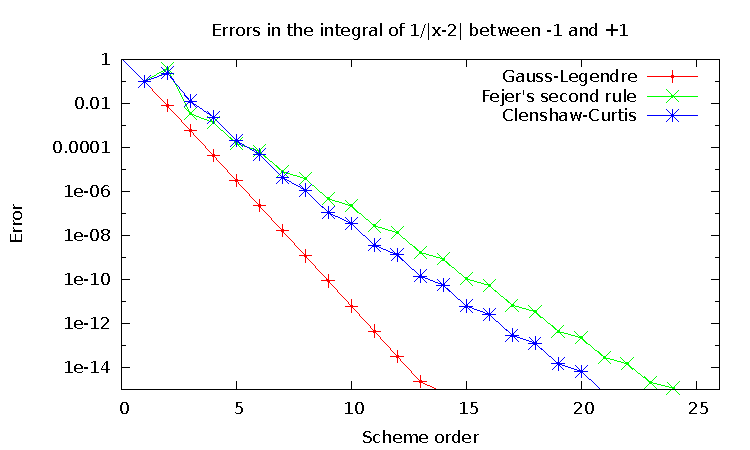
\includegraphics[width=0.75\textwidth]{./quadrature/images/quadrature_errors_xm2}
  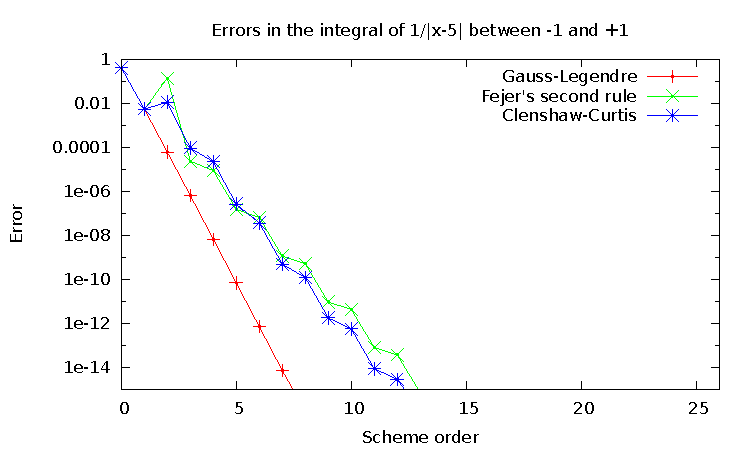
\includegraphics[width=0.75\textwidth]{./quadrature/images/quadrature_errors_xm5}
  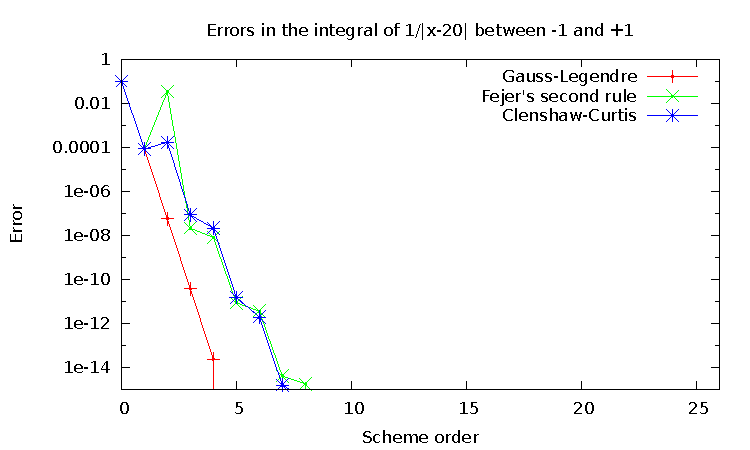
\includegraphics[width=0.75\textwidth]{./quadrature/images/quadrature_errors_xm20}
  \caption{
    \label{fig:exact_quad_errors}
    Comparison of quadrature scheme errors against analytical results in simple near-singular integrals.
  }
\end{figure}



??ds ``predictive'' vs adaptive

??ds storing values between integrations




%%% Local Variables:
%%% mode: latex
%%% TeX-master: "../lit_review_main"
%%% End:






% Notation for midpoint method stuff
% ============================================================

% notation for "at midpoint"
%% \newcommand{\valueatmidpoint}[1]{\hat{#1}}

% t at midpoint
\newcommand{\thfx}[1]{t_{#1+\half}}
\newcommand{\thf}{\thfx{n}}

% exact y of t at midpoint
\newcommand{\yvhfx}[2]{\yv#1(\thfx{#2})}
\newcommand{\yvhf}[1][]{\yvhfx{#1}{n}}

% df/dy matrix
\newcommand{\dfdy}{F}
\newcommand{\dfdyhfx}[1]{\dfdy_{#1+\half}}
\newcommand{\dfdyhf}{\dfdyhfx{n}}

% error due to midpoint approx
\newcommand{\ymiderr}{a_n}


% don't know?
%% \newcommand{\yvhfestx}[1]{\bar{\yv}_{#1}}
%% \newcommand{\yvhfest}{\yvhfestx{n}}


\section{An adaptive implicit-midpoint-rule time-integrator}


%*** other names?

%% To make the following derivations more readable we write:
%% \begin{align}
%%   \thf &= \frac{t_n + t_{n+1}}{2}, \notag\\
%%   \yvhf &= \yv(\thf), %\notag\\
%%   %% \yvhfest &= \frac{\yv_{n+1} + \yv_n}{2},
%% \end{align}
%% and we denote derivatives of $\yv$ by $\yv'$ etc.


\subsection{Fixed step implicit midpoint rule}

Let $\yv(t)$ be a vector function, let $\yv_n$ denote a vector of estimates to $\yv(t)$ at $t = t_n$.
Let $\dtn = t_{n+1} - t_n$ be the step (or time-step).
Then given a system of equations of the form
\begin{equation}
  \yv'(t) = \fv(t, \yv(t)),
  \label{eq:43}
\end{equation}
the implicit midpoint rule (IMR) is
\begin{align}
  \yv_{n+1} &= \yv_n + \dtn \fv(\frac{t_{n+1} + t_n}{2}, \frac{\yv_n + \yv_{n+1}}{2}), \notag\\
  &= \yv_n + \dtn \fv(\thf, \frac{\yv_n + \yv_{n+1}}{2}),
  \label{eq:basic-midpoint}
\end{align}
where we have written
\begin{equation}
  \frac{t_{n+1} + t_n}{2} = \thf,
\end{equation}
for readability.

Note that unlike multistep methods, such as the second order backwards difference (BDF2), this is valid for both constant and variable step sizes because there is no dependence on previous steps.


\subsection{Derivation of local truncation error}
\label{sec:deriv-local-trunc}

The local truncation error (LTE) of a time integration scheme is the error due a single integration step.
It can be calculated by substituting $\yv_n = \yv(t_n)$ into the approximation for the next time-step then subtracting the result from the exact solution at the next time-step, $\yv(t_{n+1})$.

Using this definition the local truncation error of IMR is
\begin{align}
  \lte^\IMP &= \yv(t_{n+1}) - \yv_{n+1}^\IMP, \notag\\
  &= \yv(t_{n+1}) - \yv(t_n) - \dtn \fv\left( \thf, \frac{\yv(t_n) + \yv_{n+1}^\IMP}{2} \right).
  \label{eq:trunc-start}
\end{align}

We choose to Taylor expand everything about the midpoint, $\thf$, because it reduces the complexity of the result (and allows easier calculations).\footnote{If instead chose to expand about $t_n$ there would be an additional term in $\yv_n''$ in equation~\eqref{eq:trunc-mid}.}
We assume throughout that $\yv(t)$ is ``sufficiently smooth'' to have a Taylor series expansion. Then its Taylor series expansion at $t_{n+1}$ about $\thf$ is given by
\begin{equation}
  \yv(t_{n+1}) = \yv(\thf + \frac{\dtn}{2}) = \yvhf + \frac{\dtn}{2} \yvhf['] + \frac{\dtn^2}{8} \yvhf[''] + \frac{\dtn^3}{48} \yvhf['''] \porder{\dtn^4}.
  \label{eq:taylornp1}
\end{equation}
%% It is well known that the local truncation error of the midpoint rule is $\order{\dtn^3}$ (\ie it is second order)\cite{??ds}, so we can safely ignore $\order{\dtn^4}$ terms.
Similarly the expansion at $t_n$ is
\begin{equation}
  \yv(t_n) = \yv(\thf - \frac{\dtn}{2}) = \yvhf - \frac{\dtn}{2} \yvhf['] + \frac{\dtn^2}{8} \yvhf[''] - \frac{\dtn^3}{48} \yvhf['''] \porder{\dtn^4}.
  \label{eq:taylorn}
\end{equation}

Substituting equations~\eqref{eq:taylornp1} and \eqref{eq:taylorn} into equation~\eqref{eq:trunc-start} gives
\begin{equation}
  \lte^\IMP = \yv(t_{n+1}) - \yv_{n+1}^\IMP
  = \frac{\dtn^3}{24} \yvhf[''']  + \dtn  \left[ \yvhf[']
  - \fv\left( \thf, \frac{\yv(t_n) + \yv_{n+1}}{2} \right) \right]  \porder{\dtn^4}.
  \label{eq:trunc-mid}
\end{equation}

There are two parts to this error: the first term (with $\yv'''_n$) is fairly standard in second order time integrators.
However the second term is more complex, applying a Taylor expansion approach here would result in a Jacobian-like matrix of derivatives of $\fv$ with respect to $\yv$.
Hence we avoid expanding it further.
See Section~\ref{sec:full-imr-lte-calculation} for details of the rest of the Taylor expansion which proves that IMR is indeed a second order method.



\subsection{Construction of an adaptive scheme}

Most adaptive schemes for implicit integrators (e.g. trapezoid rule, BDF2) use a Milne-device based method.\cite{gresho-sani} % not sure what page
However due to the complexity of the local truncation error of the implicit midpoint rule there are some difficulties, see Section~??ds for more details.
Instead we take the approach commonly used in Runge-Kutta time integrators: we attempt to cheaply repeat the calculation at a higher accuracy and compare the answers to get an error estimate.
Such approaches usually rely on ``Runge-Kutta pairs'', pairs of RK methods which share a number of evaluation points but have different orders of accuracy.
Examples are ??ds RK45, RK23 \cite{??ds}

However IMR uses a single evaluation at the optimal point in the time step to cause cancellation of higher order terms.
Hence there is no way to reuse this evaluation in a higher order method without at least two additional evaluations, due to the destruction of symmetry.
Instead we use a little known explicit version of the third order backwards difference method (eBDF3).
This requires only 3 history values and a single (explicit) derivative function evaluation at time $t_n$ in order to compute a 3rd order accurate step.
Alternatively a 3rd order Adams-Bashforth scheme could be used, this would require one less startup step but would require storage of an additional derivative value.




\subsubsection{Computing the size of the next time-step}

We use a standard method for computing the next time step from the local truncation error and a target local truncation error \toltt:\cite[pg.268]{Gresho-Sani}
\begin{equation}
\dtx{n+1} = \dtn \left( \frac{\toltt}{\lte^\IMP}  \right) ^{\frac{1}{3}}
\end{equation}


\subsection{Numerical experiments}

To demonstrate the effectiveness of the adaptation scheme we use a simple ODE with known exact solution
\begin{align}
  f(t,y) &= - \beta e^{-\beta t} \sin(\omega t) + \omega e^{-\beta t} \cos(\omega t) \\
  y(0) &= 0
\end{align}
which gives the exact solution
\begin{equation}
  \label{eq:59}
  y(t) = e^{-\beta t} \sin(\omega t).
\end{equation}
The numerical experiments below all use $\omega = 2 \pi$ and $\beta = 0.3$.
The exact solution for this case is shown in Figure~\ref{fig:mp-ode-exact}.
Plots of the solutions given by the various numerical calculations below are all visually indistinguishable from Figure~\ref{fig:mp-ode-exact} (without zooming in) at the tolerances used, so they are not shown.

Unless otherwise specified all examples in this section use a Newton tolerance of $1\E{-8}$ and an adaptive integrator tolerance of $\toltt = 1\E{-4}$.

\begin{figure}[ht!]
  \centering
  \includegraphics{images/osc_damped_ode_exact}
  \caption{A plot of equation~\eqref{eq:59}, the exact solution of our example ODE.}
  \label{fig:mp-ode-exact}
\end{figure}

\begin{figure}[ht!]
  \centering
  
\includegraphics{images/placeholder}
  \caption{Adaptive IMR vs adaptive BDF2 for a simple ODE.}
  \label{fig:mp-vs-bdf2}
\end{figure}

Figure~\ref{fig:mp-vs-bdf2} shows the performance of the adaptive midpoint scheme derived above compared to a standard adaptive BDF2 scheme.\cite{Gresho-Sani} %pg 715
The step size selection of the adaptive midpoint scheme closely follows that of the BDF2 scheme.


??ds discuss more about third derivative!
The pattern of step sizes is as expected.
There is a general trend of increasing step size as the solution is gradually damped out.
Additionally there is an oscillation which peaks at integer and half-integer times, this corresponds to the peaks in $\cos(\omega t)$ and $\sin(\omega t)$.
This is relevant because the truncation error is proportional to $y'''(t)$ which consists of terms in these two functions.

Also of note is that the accuracy of IMR is much higher than that of BDF2 for the same step size in this example.
??ds why? (Jacobian is zero)


Figure~\ref{fig:mp-tols} compares mean error norms and step sizes of the adaptive midpoint scheme (with two interpolation points) for varying tolerances.
The IMR can be seen to have quadratic convergence by comparing with the $y=x^2$ line shown.
Additionally it can be seen that decreasing the tolerance smoothly decreases the mean error (by smoothly decreasing the mean step size).

\begin{figure}[ht!]
  \centering
  
\includegraphics{images/placeholder}
  \caption{Adaptive midpoint mean dt vs mean error for varying tolerance. The line is $y = x^2$.}
  \label{fig:mp-tols}
\end{figure}


\subsection{Additional Notes}

\subsubsection{Implicit ODEs}
\label{sec:extens-impl-odes}

We sometimes wish to solve a system of equations where $\yv'(t)$ only given implicitly\footnote{This use of ``implicit'' is unrelated to the notion of implicitness in the time integration scheme.} (for example the Gilbert form of the Landau-Lifshitz-Gilbert equation), in this case equation~\eqref{eq:43} becomes
\begin{equation}
  \fv(t, \yv(t), \yv'(t)) = 0.
\end{equation}

We note that equation~\eqref{eq:basic-midpoint} can also be written in the from
\begin{equation}
  \yv'(\thf) = \frac{\yv_{n+1} - \yv_n}{\dtn} =  \fv(\thf, \frac{\yv_n + \yv_{n+1}}{2}).
\end{equation}
So the obvious equivalent for IMR is
\begin{equation}
  \fv(\thf, \frac{\yv_{n+1} + \yv_n}{2}, \frac{\yv_{n+1} - \yv_n}{\dtn}) = 0.
\end{equation}

However the adaptive scheme requires an additional function evaluation.
For implicitly defined functions this is expensive, so this adaptive method is not efficient for equations which can only be defined in such a way.


\subsubsection{Full lte calculation of implicit midpoint}
\label{sec:full-imr-lte-calculation}

Continuing from equation~\eqref{eq:trunc-mid} at the end of Section~\ref{sec:deriv-local-trunc}.

In order to be able to cancel terms we now need to Taylor expand $\fv\left( \thf, \frac{\yv(t_n) + \yv_{n+1}}{2} \right)$ in $\yv$ about $\yvhf$.
Hence we need an expansion of the form
\begin{align}
  \fv(\thf, \frac{\yv(t_n) + \yv_{n+1}}{2}) &= \fv(\thf, \yvhf + \dyn),
  \notag \\
  &= \fv(\thf, \yvhf) + \dfdyhf \cdot \dyn  \porder{\dyn^2}
  \label{eq:f-taylor}
\end{align}
where $\dfdyhf = \dfdy(\thf, \yvhf)$ is a \emph{matrix} of partial derivatives of each element of $\fv$ with respect to each element of the vector $\yv$ (\ie almost a Jacobian, except without the time derivative).
Note that the $\fv$ term is multiplied by an additional factor of $\dtn$ in \eqref{eq:trunc-start}, so for this part of the derivation we can drop terms of higher order than $\order{\dtn^2}$ and still retain the same asymptotic accuracy.

We now derive the required correction $\dyn$.
From equation~\eqref{eq:f-taylor} we have
\begin{equation}
  \dyn = \frac{\yv(t_n) + \yv_{n+1}}{2} - \yvhf.
  \label{eq:51}
\end{equation}
However we cannot expand $\yv_{n+1}$ to get $\dyn$ in terms of only values at the midpoint.
So we use the LTE of IMR to rewrite equation~\eqref{eq:51} as
\begin{equation}
  \dyn = \frac{\yv(t_n) + \yv(t_{n+1}) - \lte^\IMP}{2} - \yvhf.
\end{equation}
Substituting in the Taylor expansions for $\yv(t_n)$ and $\yv(t_{n+1})$ about $\thf$ (from equations~\eqref{eq:taylornp1} and \eqref{eq:taylorn}) gives
\begin{align}
  \dyn &= \yvhf + \frac{\dtn^2}{8} \yvhf[''] - \yvhf - \frac{1}{2} \lte^\IMP \porder{\dtn^4} \notag\\
  &= \frac{\dtn^2}{8} \yvhf[''] - \frac{1}{2} \lte^\IMP \porder{\dtn^4}
  \label{eq:dy-value}
\end{align}



Substituting the above value for $\dyn$ into the Taylor series expansion of $\fv$ from \eqref{eq:f-taylor} gives
\begin{equation}
  \fv(\thf, \frac{\yv(t_n) + \yv_{n+1}}{2}) = \yvhf[']
  + \frac{\dtn^2}{8} \dfdyhf \cdot \yvhf[''] - \frac{1}{2} \dfdyhf \cdot \lte^\IMP \porder{\dtn^4}
  . \label{eq:fy-taylor}
\end{equation}
and using \eqref{eq:fy-taylor} in \eqref{eq:trunc-mid} gives the local truncation error
\begin{align}
  (I + \frac{\dtn}{2}\dfdyhf) \cdot\lte^\IMP
  &= \dtn \yvhf['] + \frac{\dtn^3}{24} \yvhf[''']
  - \dtn \yvhf[']
  - \frac{\dtn^3}{8} \dfdyhf \cdot \yvhf[''] \porder{\dtn^4}
  \notag \\
  &= \frac{\dtn^3}{24} \left[\yvhf['''] - 3 \dfdyhf \cdot \yvhf[''] \right]
  \porder{\dtn^4}.
  \label{eq:trunc-implicit-form}
\end{align}

Using a geometric series representation we can show that if all eigenvalues of  $-\frac{\dtn}{2}\dfdyhf$ are s.t. $\abs{\lambda} < 1$\cite{??ds} (which will always be true for some ``small enough'' $\dtn$) then
??ds can we divide by the largest eigenvalue somewhere to do this?
\begin{equation}
  (I + \frac{\dtn}{2}\dfdyhf)^{-1} = I - \frac{\dtn \dfdyhf}{2}  \porder{\dtn^2},
\end{equation}
and so\footnote{Assuming that $\dfdyhf$ is not inversely proportional to $\dtn$.}
\begin{equation}
  \lte^\IMP = \frac{\dtn^3}{24} \left[\yvhf['''] - 3 \dfdyhf \cdot \yvhf[''] \right]
  \quad +\order{\dtn^4}.
  \label{eq:trunc-final}
\end{equation}



\section{Application of the adaptive implicit midpoint rule to micromagnetics}

%*** Banas' work

\subsection{Why use the implicit midpoint rule}

Implicit midpoint rule is known to be especially effective for micromagnetics problems \cite{DAquino2005}.
The non-dimensionalised form of the Landau-Lifshitz equation is
\begin{equation}
  \label{eq:llg-prop-form}
  \dmdt = - \mv \times( \hv - \dampc \dmdt),
\end{equation}
where $\hv$ is the effective field due to various effects depending on the system being modelled.
It is mathematically equivalent to the Landau-Lifshitz equation (as used elsewhere) with different constants, however certain properties are easier to prove with this Gilbert form so we will use it for this section.

It has certain properties:
\begin{itemize}
\item conserves magnetisation length
\item dissipates energy at a rate determined by alpha (as defined by a Rayleigh dissipation functional)
\item conserves energy at zero damping.
\end{itemize}

Clearly it is advantageous for a time discretisation method to preserve these properties.
IMR conserves them (demonstrated below), most other time discretisation schemes don't.

Errors in both of these conservation properties have been used as an error estimator for the entire error.
Hence it seems likely that reducing these errors will reduce the total error.

Geometric (or symplectic) integration schemes typically result in much smaller error build-up than schemes that do not preserve such quantities.


In addition to these properties IMR is:
\begin{itemize}
\item second order accurate -- typically considered good enough for pdes (higher orders would require expensive high order spatial discretisation to be effective, generally better to just do h-refinement instead) \cite{Matthias}
\item ??ds-stable - think it's A-stable? \cite{??ds} -- so appropriate for stiff problems, llg is stiff in some/most cases\cite{??ds}.
\end{itemize}

However it might suffer from order reduction ??ds Read more about implicit runge kutta etc?

Since IMR is a single step method there is no dependence on $\dtx{n-1}$ (unlike, for example, BDF2) and so no change in these properties would be expected when going from fixed to varying time step sizes.

\subsection{Properties of continuous Landau-Lifshitz-Gilbert equation}
\label{sec:prop-cont-llg}

We will use the identity
\begin{equation}
  \label{eq:dot-cross-id}
  \ip{\av}{\av \times \bv} = 0,
\end{equation}
which is true for all inner products because $\av \times \bv$ is perpendicular to $\av$ by the definition of the cross product.

Conservation of magnetisation length can be shown by taking the dot product (scalar product, pointwise inner product) with $\mv$ on both sides of~\eqref{eq:llg-prop-form} and using~\eqref{eq:dot-cross-id} to get
\begin{equation}
  \label{eq:56}
  \mv \cdot \dmdt = 0.
\end{equation}
Hence the change in $\mv$ is always perpendicular to $\mv$ so length is conserved.

The energy change properties can be examined similarly by taking the $L^2$ inner product
\begin{equation}
  \ip{u}{v} = \int_\magd u v \d\magd
\end{equation}
with $\hv - \dampc \dmdt$ on both sides of~\eqref{eq:llg-prop-form} and using the identity~\eqref{eq:dot-cross-id} to get
\begin{equation}
  \label{eq:58}
  \ip{\hv}{\dmdt} - \dampc \ip{\dmdt}{\dmdt} = 0.
\end{equation}
Using the fact that $\hv = -\vd{\e}{\mv}$ and the chain rule for variational derivatives\cite{??ds} we get
\begin{align*}
  \pd{\e[\mv(\xv, t), t]}{t} &= \ip{\vd{e}{\mv}}{\dmdt} - \ip{\pd{\happ}{t}}{\mv} \\
             &= -\ip{\hv}{\dmdt} - \ip{\pd{\happ}{t}}{\mv},
\end{align*}
and so
\begin{equation}
  \ip{\hv}{\dmdt} = -\vd{\e}{t} - \ip{\pd{\happ}{t}}{\mv}.
\end{equation}

Substituting this into equation~\eqref{eq:58} leaves
\begin{equation}
  \label{eq:energy-decay}
  \vd{\e}{t} = -\dampc \ip{\dmdt}{\dmdt} - \ip{\pd{\happ}{t}}{\mv}.
\end{equation}

Equation~\eqref{eq:energy-decay} shows that under constant applied field the energy of the system is always decreasing by an amount proportional to $\dampc$.
In fact this relationship is the Rayleigh dissipation functional used as the basis for the derivation of the Gilbert form of the LLG.\cite{Gilbert2004}
For non-constant applied fields the change in the Zeeman energy is added which may increase or decrease the energy depending on how the field is changed. % field moves towards m -> decrease, away -> increase. For non-spatially constant this is averaged over space in some sense by the inner product.


\subsection{Properties of midpoint method LLG discretisation}
\label{sec:prop-midp-meth}

??ds discuss which inner products/norms are used where

As noted in Section~\ref{sec:extens-impl-odes} IMR is defined by the following substitutions
\begin{align}
  \label{eq:55}
  \pd{\mv}{t} &= \frac{\mv_{n+1} - \mv_n}{\dtn}, \\
  \mv &= \frac{\mv_{n+1} + \mv_n}{2}, \\
  t &=  \frac{t_{n+1} + t_n}{2}.
\end{align}

The special conservation properties of IMR discretisation of the Landau-Lifshitz-Gilbert equation come from the fact that for any symmetrical linear operator $\ell$
\begin{align}
  \label{eq:54}
  \ip{\ell \left[ \mv_{n+\half} \right]}{ \pd{\mv}{t} \lvert_{n+\half}}
  &= \frac{1}{2\dtn} \left[
    (\mv_{n+1} , \ell \mv_{n+1})
    + (\mv_{n+1} , \ell \mv_{n})
    - (\mv_{n} , \ell \mv_{n+1})
    - (\mv_{n} , \ell \mv_{n})
    \right] \notag\\
  &= \frac{1}{2\dtn} \left[
    (\mv_{n+1} , \ell \mv_{n+1})
    - (\mv_{n} , \ell \mv_{n})
    \right].
\end{align}

In particular for the identity operator, $\mv \in \real$ and $(\av, \bv) = \av \cdot \bv$ we have
\begin{equation}
  \label{eq:52}
  \mv \cdot \pd{\mv}{t}  = \frac{1}{2\dtn} (\norm{\mv_{n+1}}^2 - \norm{\mv_{n}}^2 ).
\end{equation}
Substituting this into equation~\eqref{eq:56} gives
\begin{equation}
  \abs{\mv_{n+1} }^2 - \abs{\mv_{n}}^2 = 0 \quad \forall \xv \in \magd
\end{equation}
\ie conservation of magnetisation length.

??ds operators below need checking, dAquino is only concerned with FD...

The time-discretised effective field can be represented as a symmetrical linear operator on magnetisation:\cite{DAquino2005}
\begin{equation}
  \label{eq:hop}
  \hv_n(\xv) = \hop [\mv_n(\xv)] + \happ(\xv, t_n).
\end{equation}
Additionally the energy can be written using this operator as
\begin{equation}
  \label{eq:energy-hop}
  \e_n = \frac{1}{2} \ip{\mv_n}{\hop[\mv_n] + \happ(\xv,t_n)}.
\end{equation}

Substituting the midpoint approximation and equation~\eqref{eq:hop} into \eqref{eq:58} leaves
\begin{align}
  \label{eq:60}
  &\ip{ \pd{\mv}{t} \lvert_{n+\half}}{\hop \left[\mv_{n+\half} \right]} + \ip{\frac{\mv_{n+1} - \mv_n}{\dtn}}{\happ(\xv,t_{n+\half})} \\
  &= \dampc \ip{\frac{\mv_{n+1} - \mv_n}{\dtn}}{\frac{\mv_{n+1} - \mv_n}{\dtn}}.
\end{align}
We use a midpoint approximation for the applied field to allow us to cancel terms later:
\begin{equation}
  \label{eq:happ-midpoint}
  \happ(\xv,t_{n+\half}) = \frac{\happ(\xv, t_{n+1}) + \happ(\xv, t_n)}{2} + \order{\dtn^2 \spd{\happ}{t}}.
\end{equation}
Combining equations~\eqref{eq:60}, \eqref{eq:happ-midpoint} and the identity~\eqref{eq:54} gives us
\begin{align}
  &\frac{\ip{\mv_{n+1}}{\hop \left[\mv_{n+1} \right] + \happ(\xv, t_{n+1})}
    - \ip{\mv_{n}}{\hop \left[\mv_{n} \right] + \happ(\xv, t_n)}
    }{2\dtn} \notag\\
  &= \dampc \norm{\frac{\mv_{n+1} - \mv_n}{\dtn}}^2
  + \order{\dtn^2 \spd{\happ}{t}}.
\end{align}
After substitution of the energy from~\eqref{eq:energy-hop} this leaves
\begin{equation}
  \frac{\e_{n+1} - \e_n}{\dtn}
  = \dampc \norm{\frac{\mv_{n+1} - \mv_n}{\dtn}}^2
  + \order{\dtn^2 \spd{\happ}{t}}.
\end{equation}
Hence with (piecewise) linear applied fields the energy loss is exactly correct.

It should be noted that the above properties are only true up to the accuracy with which we solve the LLG. Since the LLG is non-linear this is typically the Newton tolerance.


\subsection{Numerical Experiments}

In this section we present numerical experiments showing that the adaptive midpoint method retains the conservation properties of the fixed step midpoint method.
For this purpose we choose a simple model: a small\footnote{Small enough that exchange coupling dominates and the magnetisation is spatially constant throughout the particle.} spherical nano-particle with no magnetocrystalline anisotropy under linearly increasing applied field.
In this case
\begin{equation}
  \hv(t) = - t/2 +  \frac{\mv}{3}.
\end{equation}
The initial magnetisation used is $\mv_0 = \left( 0.05, 0, \sqrt{1 - 0.05^2} \right)$.
The damping constant is $\dampc = 0.3$.
The Newton tolerance is $1\E{-8}$ and the adaptive integrator tolerance is $\toltt = 1\E{-4}$ unless otherwise specified.

Figure~\ref{fig:linear-field-switch-mp} shows again that the adaptivity works: initially the field is so weak that not much is happening and large steps are taken.
Then the switching speeds up and the step size gradually decreases.
Finally the switching is finished and the step size increases again.

\begin{figure}[ht!]
  \centering
  
\includegraphics{images/placeholder}
  \caption{Magnetisation dynamics and step size selections for a small spherical magnetic nano-particle switching in a linearly increasing applied field. Calculated using the adaptive midpoint method with two interpolation points.}
  \label{fig:linear-field-switch-mp}
\end{figure}

Figure~\ref{fig:linear-field-switch-errors-mp} shows that the adaptive midpoint method gives orders of magnitude better accuracy than adaptive BDF2 in magnetisation length and effective damping, as expected.
Of interest is the noise in the midpoint effective damping error between $t \approx 2.5$ and $t \approx 9$.
This is caused by strong variation in the final Newton error: since Newton's method gives quadratic convergence one additional step results in orders of magnitude more accuracy.
This also indicates that the errors are strongly related to the Newton solver error, which is as expected since this is the only source of error (in these quantities) which is not removed by the use of IMR.

??ds also do fixed step midpoint?

\begin{figure}[ht!]
  \centering
  
\includegraphics{images/placeholder}
  \caption{Comparison of errors in $\abs{\mv}$ and $\dampc$ for adaptive midpoint method and adaptive BDF2 for a small spherical magnetic nano-particle switching in a linearly increasing applied field.}
  \label{fig:linear-field-switch-errors-mp}
\end{figure}


To investigate this effect further we compare the average errors for various Newton tolerances in Figure~\ref{fig:newton-tol-errors-mp}.
It can be seen that reduction of the Newton tolerance strongly reduces the mean errors.

\begin{figure}[ht!]
  \centering
  
\includegraphics{images/placeholder}
  \caption{Effect of varying the Newton method tolerance on errors in $\abs{\mv}$ and $\dampc$  for the switching nano-particle problem discussed above.}
  \label{fig:newton-tol-errors-mp}
\end{figure}


\subsection{Discussion}

\subsubsection{Extension to pdes}

We have done some initial work using adaptive midpoint for the non-spatially constant LLG (\ie a pde) which works well for fully implicit problems.

Unfortunately the energy/damping conservation properties require the entire calculation to be performed implicitly.
This is incompatible with the semi-implicit FEM/BEM method for magnetostatic field calculations,\cite{Koehler1997} which is used in the current implementation of our model.
However d'Aquino \etal demonstrated an efficient, fully implicit finite difference LLG solver using the fixed step midpoint method\cite{DAquino2005}.
Such a solver should be easily to modifiable to use our adaptive midpoint method.

The conservation of magnetisation length by IMR does not require a fully implicit calculation as demonstrated by Spargo \etal\cite{Spargo2003a}.
Hence the adaptive midpoint method could be used to construct a semi-implicit magnetisation-length-conserving scheme with purely numerical time adaptivity, with the advantages discussed in Section~\ref{sec:altern-time-adapt}.


\subsubsection{Alternative time adaptivity methods in micromagnetics}
\label{sec:altern-time-adapt}

In cases where the damping is not exact the effective damping can be used as an error estimator, as proposed by Albuquerque \etal\cite{Albuquerque2001}
??ds The disadvantage of this method (aside from the obvious requirement that the damping be inexact) is that, depending on the discretisation used, the error estimator may be unable to distinguish between insufficient space refinement and insufficient time refinement.
In particular this is the case when the solution is not completely divided into separate effective field calculations and pointwise time integration, such as in a typical Galerkin finite element model.

Rigorous time error estimates for the LLG with limited effective field terms with a certain discretisation method were proven and used to perform adaptive refinement of midpoint method time steps by Banas.\cite{Banas-thesis} ??ds do these work, why does no one use them?
By comparison our adaptive method is much more general in that it can be applied to any differential equation and any discretisation scheme which uses the method of lines for time.

\subsubsection{Symplecity}

??ds I basically have no idea about this stuff.

The fixed step midpoint method is ``almost symplectic'' for the LLG equation with zero damping (Hamiltonian structure is preserved up to a small error).\cite{Austin1993}
However it is well known that most adaptive schemes are not symplectic\cite{Iserles2009} % pg. 91
because they constantly change the nearby Hamiltonian that is followed by the symplectic integrator.

??ds MORE


\subsection{Future work}

%*** Does adaptivity trail off eventually like trapazoid?

Testing with pdes.



%%% Local Variables:
%%% mode: latex
%%% TeX-master: "./main"
%%% End:


%  preconditioners:
% (very) basicis
% what have people done before?

%  LLB/ heat flow modelling
% very basics
% what have people done before?

\appendix

\chapter{A note on the signs of the Landau--Lifshitz--Gilbert equation}
\label{sec:note-signs-llg}

In the recent republication of Gilbert's derivation of the
Landau--Lifshitz--Gilbert equation\cite{Gilbert2004} (originally from his
thesis) he gives the following equivalent equations:
\begin{equation}
  \pd{\Mv}{t} = - \abs{\gamma} \Mv \times \big[ \Hv - \eta \pd{\Mv}{t} \big],
\end{equation}
and
\begin{equation}
  \pd{\Mv}{t} = - \abs{\gamma} \Mv \times \Hv - \frac{\alpha}{M_s} \Mv \times \pd{\Mv}{t}.
  \label{eq:llg-vedamping}
\end{equation}
Where $\alpha = \eta \gamma M_s$ and $\gamma < 0$. However the sign of $\eta$ is not given, hence the sign of $\alpha$ is not certain. Conventionally the sign of $\alpha$ is positive but since Gilbert's paper was probably the first to use that constant he may have used a different convention.

Another potential source of confusion is the sign of $\gamma$. Physically the gyromagnetic constant for an electron is negative. However some authors use $\gamma$ to represent $\abs{\gamma}$, thus reversing some signs.

Many more recent sources\cite{Fidler2000}\cite{nmag-manual}\cite{Lopez-Diaz2012} give the Landau-Lifshitz-Gilbert equation as
\begin{equation}
  \pd{\Mv}{t} = - \abs{\gamma} \Mv \times \Hv + \frac{\alpha}{M_s} \Mv \times \pd{\Mv}{t},
  \label{eq:llg+vedamping}
\end{equation}
note the opposite sign on the second term. I think this discrepancy is due to opposite conventions in the sign of $\alpha$.

Additionally Mallinson notes in his paper on Damped Gyromagnetic Switching\cite{Mallinson2000} that ``a certain degree of confusion exists concerning what are the correct algebraic signs to be used in [the LLG] equation''. He asserts that equation \eqref{eq:llg+vedamping} is correct and notes that many of his previous papers used the incorrect sign.\footnote{Unfortunately this same paper contains a misprint in its statement of the LLG, a factor of $\bar{H}_f$, along with some other errors all given in a later errata.}


Hence we will use equation \eqref{eq:llg+vedamping}.




%%% Local Variables:
%%% mode: latex
%%% TeX-master: "main"
%%% End:


\section{Non-dimensionalisation}
\label{sec:normalisations-appendix}

%??ds talk about why?

% no unecessary (for the maths) parameters
% improves accuracy by minimising round off error

\subsection{The Landau-Lifshitz-Gilbert equation}
\label{sec:land-lifsh-gilb-normalisation}

We start from the Landau--Lifshitz--Gilbert equation with the magnetostatic, applied, exchange and magnetocrystalline (effective) fields (see Section~\ref{sec:cont-micromag}):

\begin{align}
  \pd{\Mv^*}{t^*} &= - \gymagc \Mv^* \times \Hv^* + \frac{\alpha}{M_s} \Mv^* \times \pd{\Mv^*}{t^*}, \label{eqn:llgnd} \\
  \Hv^* &= \Happ^* - \nabla^* \phi^* + \frac{2\Exchc^*}{\mu_0 M_s} \nabla^{*2} \mv + \frac{2\Kone^*}{\mu_0 M_s} (\mv \cdot \ev) \ev.
  \label{eqn:effnd} \\
  \nabla^{*2} \phi^* &= \nabla^* \cdot \Mv^* \label{eqn:phind}
\end{align}
where we use $^*$ to denote the dimensional variables, operators and constants that will be non-dimensionalised. We assume (for simplicity) that $M_s$, $\Exchc$ and $\Kone$ are all
constant throughout the magnetic materials used.

Let
\begin{align}
  \Mv^* &= M_s \mv, \notag \\
  \phi^* &= \Phi \phi, \notag \\
  \Hv^* &= M_s \hv, \label{eqn:nddefs} \\
  \Exchc^* &= \nA \exchc, \notag \\
  \Kone^* &= \nK \kone, \notag \\
  t^* &= \frac{1}{\gymagc M_s} t, \notag \\
  x_i^* &= l x_i. \notag
\end{align}
Note that $\Mv$ and $\Hv$ have the same units so we use the same normalisation factor. For dimensional purposes derivatives are equivalent to division by the variable differentiated with respect to, so $\nabla^* = \frac{1}{l} \nabla$, $\pd{a}{t^*} = \gymagc M_s \pd{a}{t}$ etc.

Combining equation~\eqref{eqn:llgnd} with the definitions~\eqref{eqn:nddefs} gives
\begin{equation}
  \notag
  \dmdt \gymagc M_s^2 =
  - \gymagc M_s^2 (\mv \times \hv) + \frac{\alpha}{M_s} \gymagc M_s^3 (\mv \times \dmdt),
\end{equation}

cancelling the various constants results in the non-dimensionalised Landau--Lifshitz--Gilbert equation
\begin{equation}
  \label{eq:53}
  \dmdt = - (\mv \times \hv) + \alpha (\mv \times \dmdt).
\end{equation}

Similarly for equation~\eqref{eqn:phind}
\begin{align*}
  \frac{1}{l^2} \Phi \nabla^{2} \phi &= \frac{1}{l} M_s \nabla \cdot \mv, \\
  \frac{\Phi}{M_s l} \nabla^{2} \phi &= \nabla \cdot \mv.
\end{align*}

Letting $\Phi = M_s l$ we obtain
\begin{equation}
  \label{eq:57}
  \nabla^2 \phi = \nabla \cdot \mv.
\end{equation}

Repeating the substitutions for equation~\eqref{eqn:effnd} gives
\begin{align*}
  M_s \hv &= M_s \happ - \frac{\Phi}{l} \nabla \phi + \frac{2\nA}{\mu_0l^2 M_s}  \exchc \nabla^2 \mv + \frac{2\nK}{\mu_0 M_s}  \kone (\mv \cdot \ev) \ev, \\
  \hv &= \frac{M_s}{M_s} \happ - \frac{M_s}{M_s} \nabla \phi + \frac{2\nA}{\mu_0 l^2 M_s^2}  \exchc \nabla^2 \mv + \frac{2\nK}{\mu_0 M_s^2} \kone (\mv \cdot \ev) \ev.
\end{align*}
This can be further simplified by using:
\begin{align}
  \nK &= \mu_0 M_s^2, \notag \\
  \nA &= l^2 \nK, \label{eqn:ndfields}
\end{align}

leaving
\begin{equation}
  \hv = \happ - \nabla \phi + 2\exchc \nabla^2 \mv + 2\kone (\mv \cdot \ev) \ev.
\end{equation}

The parameter for length, $l$ is still free to be chosen. Useful possibilities are the exchange length or a unit on the length scale of a dimension of the magnetic material being modelled (typically $\sim1-100$nm).


\subsection{Energy calculations}
\label{sec:energy-calculations}

Sometimes we may need to know the non-dimensional energy of a micromagnetic state in a form consistent with that used for the LLG equation. One example is for the computation of an effective damping constant, see section ??ds.

We repeat the process used in Section~\ref{sec:land-lifsh-gilb-normalisation} to get a set of non-dimensionalised energy equations, starting from the equations given in Section~\ref{sec:energy-magnetic-body}:

\begin{equation*}
  \Eapp^* = - \mu_0 \int_{\magd} \Mv^* \cdot \Happ^* \d \magd^*,
\end{equation*}
\begin{equation}
  \Ems^* =  \frac{-\mu_0}{2} \int_{\magd} \Mv^* \cdot \Hms^* \d \magd^*,
\end{equation}
\begin{equation*}
  \Eex^* =  \Exchc^* \int_{\magd} (\nabla^* \mv)^2 \d \magd^*,
\end{equation*}
\begin{equation*}
  \Eca^* =  \Kone^* \int_\magd (\mv \cdot \ev)^2 \d \magd^*.
\end{equation*}

We substitute definitions~\eqref{eqn:nddefs}, \eqref{eqn:ndfields} and $E^* = \nE e = \mu_0 M_s^2 l^d \, e$ where $d$ denotes the number of spatial dimensions:
\begin{equation*}
  \eapp = \frac{-\mu_0 M_s^2 l^d}{\nE} \int_{\magd} \mv \cdot \happ \d \magd
  = - \int_{\magd} \mv \cdot \happ \d \magd,
\end{equation*}
\begin{equation}
  \ems = \frac{-\mu_0 M_s^2 l^d}{2\nE} \int_{\magd} \mv \cdot \hms \d \magd
  = - \int_{\magd} \mv \cdot \hms \d \magd,
\end{equation}
\begin{equation*}
  \eex =  \frac{\mu_0 M_s^2 l^2 l^d}{l^2\nE} \exchc \int_{\magd} (\nabla \mv)^2 \d \magd
  = \exchc \int_{\magd} (\nabla \mv)^2 \d \magd,
\end{equation*}
\begin{equation*}
  \eca = \frac{\mu_0 M_s^2 l^d}{\nE} \kone \int_\magd 1 - (\mv \cdot \ev)^2 \d \magd
  = \kone \int_\magd 1 - (\mv \cdot \ev)^2 \d \magd.
\end{equation*}
Note that we have used
\begin{equation}
  \d \magd^* = \d x^{*d} = l^d \d x^d = l^d \d \magd.
\end{equation}



%%% Local Variables:
%%% mode: latex
%%% TeX-master: "main"
%%% End:

\section{Analytical solutions of the Landau-Lifshitz-Gilbert equation}

When testing numerical solvers for differential equations it is very
helpful to be able to check the results against analytical solutions for
some special cases. This section contains some solutions useful for this
purpose.
Unfortunately it appears to be very difficult to find solutions to the LLG equation with exchange coupling (i.e. spatially dependant/spatially non-constant).

\subsection{Solution due to Mallinson}

In a 2000 paper\cite{Mallinson2000} Mallinson gives an analytical equation for the time taken for magnetisation to ``switch'' from one polar angle (angle to the field axis) to another.
He also gives the azimuthal angle (the angle around the field axis) rotated through during this switching.

The conditions for this model to apply are:
\begin{enumerate}
\item Constant applied field.
\item No exchange field.
\item Uniaxial anisotropy.
\item Magnetostatic field (prolate ellipsoidal particles only).
\item All effective fields must lie along the same axis.
\end{enumerate}

Let $\theta_1$, $\theta_2$ be the starting and endingangles between the field axis and the magnetisation (i.e. polar angles). Let $H_k$ be the combined anisotropy field: $H_k = \frac{2 K}{M_s} + M_s(N_\perp - N_\parallel)$ where $N$ is the demagnetisation tensor of the ellipsoid. All other symbols have their usual meanings. Then the time taken to switch from $\theta_1$ to $\theta_2$ is

\begin{equation}
  \tau = \frac{\dampc^2 +1}{\gymagc \dampc} \frac{1}{H^2 - H_k^2}
  \left[ H \ln \left( \frac{\tan(\theta_2/2)}{\tan(\theta_1/2)} \right)
       + H_k \ln \left( \frac{H - H_k \cos\theta_1}{H - H_k \cos\theta_2} \right)
       + H_k \ln \left( \frac{\sin\theta_2}{\sin\theta_1} \right)
    \right].
\end{equation}

The azimuthal angle precessed through during this switching is
\begin{equation}
  \phi = \frac{-1}{\dampc} \ln \left( \frac{\tan(\theta_2/2)}{\tan(\theta_1/2)} \right).
\end{equation}

Note that this is not really a true ``solution'' to the Landau-Lifshitz-Gilbert equation.
It gives the switching time and azimuthal angle as a function of polar angle rather than the magnetisation direction as a function of time.

\subsection{Solution due to ??ds}

A similar solution has been given by ... for the case when the field is applied at a right angle to the easy axis.


...



\subsection{Constant field solution}

...


\subsection{Solution with exchange}

It turns out to be possible to write down a solution to the Landau-Lifshitz-Gilbert equation even with the exchange term included as long as the physical boundary condition ??ds is ignored.

??ds don't remember the solution...


\begin{landscape}
  \begin{table}
    \centering
    \input{./other_models}
    \caption{Some key features of micromagnetic codes. The entry for oomph-lib (1) lists the features that are already available in the library (except mid-point method will be implemented). Codes (2-4) are currently available open source micromagnetics models, while numbers 5-6 are commercial, closed source packages.}
    \label{fig:other-models}
  \end{table}
\end{landscape}

%\bibliographystyle{amsalpha} %use codes instead of numbers
%% \bibliographystyle{amsplain}

% Make sure websites is before the Mendeley library as website entries needed to
% be manually adjusted but may be overridden if the Mendeley library is first in
% the list.
%% \bibliography{./websites,./library}

% Does what it says (using biblatex package)
\printbibliography

\end{document}


%%% Local Variables:
%%% mode: latex
%%% TeX-master: t
%%% End:
